\documentclass[ack,preface]{diphdthesis}

% \usepackage{amsfonts,amsmath,amssymb,latexsym}
\usepackage{bookmark}
\usepackage{caption}
\usepackage{epigraph}
\usepackage{graphicx}
\usepackage[utf8]{inputenc}
\usepackage{minted}
\usepackage{multirow}
\usepackage[defblank]{paralist}
\usepackage[skip=0cm,list=true,labelfont=it]{subcaption}
\usepackage{wrapfig}

\usepackage{styles/languages}

%%%% TEMPORARY %%%%
\usepackage{xcolor}
\usepackage{pagecolor}
%\pagecolor{black}
%\color{white}
%%%% TEMPORARY %%%%


%%%% Metadata START %%%%
\authorFirstGr{Γεώργιος}
\authorFirstAbrGr{Γ.} % abbreviation of first name
\authorMiddleGr{Σ.}   % abbreviation of father's first name
\authorLastGr{Καστρίνης}
\authorFirstEn{George}
\authorFirstAbrEn{G.}
\authorMiddleEn{S.}
\authorLastEn{Kastrinis}

\titleGr{Αποδοτική Στατική Ανάλυση Δεικτών με Αξιόπιστα Αποτελέσματα}
%\titleGr{Αποδοτικότητα και Αξιοπιστία σε Στατική Ανάλυση Δεικτών}
\titleEn{Scalable Static Pointer Analysis with High-Confidence Results}
%\titleEn{Scalability and Confidence for Static Pointer Analysis}

% Month followed by Year
\dateGr{ΔΕΚΕΜΒΡΙΟΣ 2019}
\dateEn{DECEMBER 2019}

% Advisor info
\advisorGr{Γιάννης Σμαραγδάκης}
\advisorRankGr{Καθηγητής}
\advisorOrgGr{ΕΚΠΑ}
\advisorEn{Yannis Smaragdakis}
\advisorRankEn{Professor}
\advisorOrgEn{NKUA}

% Members of the advisory board 
% (the first one, will be automatically taken up by the advisor)
\boardTwoGr{Αλέξης Δελής}
\boardTwoRankGr{Καθηγητής}
\boardTwoOrgGr{ΕΚΠΑ}
\boardTwoEn{Alex Delis}
\boardTwoRankEn{Professor}
\boardTwoOrgEn{NKUA}

\boardThreeGr{Παναγιώτης Ροντογιάννης}
\boardThreeRankGr{Καθηγητής}
\boardThreeOrgGr{ΕΚΠΑ}
\boardThreeEn{Panos Rondogiannis}
\boardThreeRankEn{Professor}
\boardThreeOrgEn{NKUA}

% 7 Member examination committee
% (the first three will be taken up by the advisory board)
%%%%%%%%%%% TEMPORARY %%%%%%%%%%%
\examFourGr{Μέμα Ρουσσοπούλου}
\examFourRankGr{Αναπληρώτρια Καθηγήτρια}
\examFourOrgGr{ΕΚΠΑ}
\examFourEn{Mema Roussopoulos}
\examFourRankEn{Associate Professor}
\examFourOrgEn{NKUA}

\examFiveGr{Μανόλης Κουμπαράκης}
\examFiveRankGr{Καθηγητής}
\examFiveOrgGr{ΕΚΠΑ}
\examFiveEn{Manolis Koubarakis}
\examFiveRankEn{Professor}
\examFiveOrgEn{NKUA}

\examSixGr{Νικόλαος Παπασπύρου}
\examSixRankGr{Αναπληρωτής Καθηγητής}
\examSixOrgGr{ΕΜΠ}
\examSixEn{Nikolaos Papaspyrou}
\examSixRankEn{Associate Professor}
\examSixOrgEn{NTUA}

\examSevenGr{???}
\examSevenRankGr{Αναπληρωτής Καθηγητής}
\examSevenOrgGr{???}
\examSevenEn{???}
\examSevenRankEn{Associate Professor}
\examSevenOrgEn{???}

% The examination date of the thesis
\examinationDateGr{30 Φεβρουαρίου 2020}
\examinationDateEn{February 30, 2020}


%%%% Abstract, synopsis, inscription, ack, and preface pages %%%%
\abstractEn{Static program analysis aims to automatically reason about certain properties a given program might exhibit under all possible executions without actually observing such executions. Static \emph{pointer} analysis is a major subcategory that focuses on the objects that program expressions might point to during program executions. The evolution of programming languages has led to the addition of many abstraction layers that, as a result, have made any automatic reasoning about a program a challenging task at best or an infeasible one at worst. Thus, any practical static pointer analysis algorithm has to compromise and aim to approximate results in some way---either computing more or less than what is actually true.

This dissertation shows how we can obtain \emph{precise} yet also \emph{scalable} static pointer analysis algorithms by carefully differentiating policies for different parts of the program. Furthermore, since a static pointer analysis algorithm with global soundness guarantees and meaningful results throughout is not realistic, we show that it is possible to design analyses that offer \emph{strong guarantees} on the soundness of the results for specific parts of the program.

Pointer analyses in the past introduced the concept of \emph{context-sensitivity} in order to tackle the ever growing problem of imprecision versus scalability. Context is used to annotate analysis components so that the analysis can be more precise without at the same time sacrificing scalability. We show beneficial ways to combine different context flavors for different parts of the program without paying the cost that a naive combination would incur.

Another attempt at producing precise yet scalable analyses leads us to an introspective analysis. We employ a common adaptive pattern in which a cheap imprecise analysis is run first so various metrics can be gathered, and then a more precise (and costly) analysis can be used only in parts of the program---under the assumption that more precise handling of the rest would only incur performance penalties.

Subsequently, we shift our attention to an analysis that \emph{under}-approximates results (instead of the norm of \emph{over}-approximating) so that it might report less but can guarantee those properties to always hold. We build upon observations on the properties that such analyses have in order to apply a specialized data structure that speeds up our algorithm by nearly two orders of magnitude.

Finally, in our last contribution, we revisit an analysis formulation that overapproximates results to create an analysis algorithm that is truly sound but at the same time highly efficient. Our analysis is conservative, guaranteeing soundness even in the presence of arbitrary unknown code, but avoids wasting any work on computations that will later be invalidated due to soundness concerns.}
\abstractGr{Η στατική ανάλυση στοχεύει στον αυτόματο συμπερασμό ιδιοτήτων που κάποιο πρόγραμμα μπορεί να επιδείξει σε κάθε πιθανή εκτέλεση, χωρίς στην πράξη να εκτελείται. Η στατική ανάλυση \emph{δεικτών} αποτελεί μια μεγάλη υποκατηγορία της που επικεντρώνεται στα δυναμικά αντικείμενα που δύνανται να ``δείξουν'' οι εκφράσεις ενός προγράμματος σε κάποια εκτέλεση του. Η εξέλιξη των γλωσσών προγραμματισμού με την πάροδο των χρόνων οδήγησε στην προσθήκη πολλών επιπέδων αφαίρεσης, τα οποία σαν αποτέλεσμα έχουν ο αυτόματος συμπερασμός για κάποιο πρόγραμμα να αποτελεί τουλάχιστον μία πρόκληση αν όχι και μία αδύνατη προσπάθεια. Συνεπώς, κάθε πρακτικός αλγόριθμος στατικής ανάλυσης πρέπει να στοχεύσει σε μια εκτίμηση των πραγματικών αποτελεσμάτων με κάποια μορφή ανακρίβειας---είτε υπολογίζοντας περισσότερα είτε λιγότερα.

Σε αυτή τη διατριβή παρουσιάζουμε πώς μπορούμε να σχεδιάσουμε \emph{ακριβείς} και συνάμα \emph{αποδοτικούς} αλγορίθμους ανάλυσης δεικτών εφαρμόζοντας διαφορετικές πολιτικές σε διαφορετικά σημεία του προγράμματος. Συμπληρωματικά, δεδομένου ότι ένας αλγόριθμος ανάλυσης δεικτών με βεβαιώσεις εγκυρότητας για όλα τα σημεία του προγράμματος καθώς και πρακτικά αποτελέσματα δεν αποτελεί ρεαλιστική κατεύθυνση, δείχνουμε πώς μπορούμε να σχεδιάσουμε αναλύσεις με \emph{ισχυρές βεβαιώσεις εγκυρότητας} για συγκεκριμένα κομμάτια ενός προγράμματος.

Προηγούμενοι αλγόριθμοι για ανάλυση δεικτών εισήγαγαν την έννοια των \emph{συμφραζομένων} ({\en context}) για να αντιμετωπίσουν το αυξανόμενο πρόβλημα της ανακρίβειας έναντι της αποδοτικότητας. Τα συμφραζόμενα χρησιμοποιούνται για να επαυξήσουν στοιχεία της ανάλυσης ώστε η ανάλυση να καταφέρει να είναι πιο ακριβής χωρίς ταυτόχρονα να πρέπει να κάνει θυσίες στον τομέα της αποδοτικότητας. Παρουσιάζουμε επωφελείς τρόπους συνδυασμού διάφορων ειδών συμφραζομένων σε διαφορετικά σημεία του προγράμματος, χωρίς αυτοί οι συνδυασμοί να επιφέρουν το κόστος που θα παρουσίαζε μία αφελής προσέγγιση.

Μία δεύτερη απόπειρα για δημιουργία αναλύσεων που παρουσιάζουν υψηλή ακρίβεια και αποδοτικότητα μας οδηγεί σε μια ανάλυση \emph{ενδοσκόπησης} ({\en introspection}). Εφαρμόζουμε ένα σύνηθες μοτίβο στο οποίο μια φτηνή ανακριβής ανάλυση εφαρμόζεται πρώτη ώστε να συλλέξει διάφορες μετρικές για το πρόγραμμα, και στη συνέχεια μια δεύτερη πιο ακριβής (και ακριβή) ανάλυση μπορεί να εφαρμοστεί μόνο σε συγκεκριμένα σημεία του προγράμματος---υπό την υπόθεση ότι η πιο ακριβής μεταχείριση των υπολοίπων θα είχε μόνο αρνητικά αποτελέσματα στην συνολική απόδοση.

Εν συνεχεία, μετατοπίζουμε την προσοχή μας προς μια ανάλυση που \emph{υπό}-εκτιμά τα αποτελέσματα της (σε αντίθεση με το σύνηθες των αναλύσεν που υπολογίζουν μία \emph{υπέρ}-εκτίμηση). Με αυτή την αντιμετώπιση, η ανάλυση μας αναφέρει λιγότερα αποτελέσματα αλλά μπορεί να παρέχει ισχυρές βεβαιώσεις ότι αυτά θα ισχύουν πάντα. Βασιζόμενοι πάνω σε παρατηρήσεις για τις ιδιότητες που παρουσιάζουν αναλύσεις αυτού του είδους, εφαρμόζουμε μια ειδική δομή δεδομένων η οποία επιφέρει επιταχύνσεις στον αλγόριθμο μας σχεδόν κατά δύο τάξεις μεγέθους.

Τέλος, στην τέταρτη συνεισφορά της διατριβής, επιστρέφουμε ξανά στην οικογένεια αναλύσεων που υπερεκτιμούν τα αποτελέσματα τους. Ο στόχος μας είναι η δημιουργία ενός αρκετά αποδοτικού αλγορίθμου που όντως παράγει έγκυρα αποτελέσματα χωρίς περιορισμούς στο υποκείμενο πρόγραμμα. Κατά συνέπεια, αυτό μας οδηγεί σε μία συντηρητική ανάλυση, που μπορεί να παρέχει βεβαιώσεις εγκυρότητας ακόμα και ύπο την παρουσία άγνωστου κώδικα, αλλά ταυτόχρονα αποφεύγει την σπατάλη υπολογισμών σε δεδομένα που αργότερα θα χρειαστεί να ανατραπούν για την διατήρηση των βεβαιώσεων αυτών.}
\synopsisGr{Η διατριβή αυτή ανήκει στον ευρύτερο τομέα της στατικής ανάλυσης προγραμμάτων, η οποία στοχεύει στον αυτόματο συμπερασμό για τις ιδιότητες που παρουσιάζει κάποιο πρόγραμμα με βάση την εξέταση του πηγαίου του κώδικα (ή κάποιας αντίστοιχης ενδιάμεσης αναπαράστασης), αλλά δίχως να απαιτείται πραγματική εκτέλεση του. Η δουλειά μας στην διατριβή αυτή επικεντρώνεται σε μια μεγάλη υποκατηγορία της στατικής ανάλυσης, αυτή της ανάλυσης \emph{δεικτών}. Μία ανάλυση δεικτών στοχεύει στο να υπολογίσει τα σύνολα αντικείμένων στα οποία μπορεί να ``δείξει'' κάθε έκφραση του προγράμματος (π.χ. τοπική μεταβλητή, ή κάποιο πεδίο, κτλ.) σε όλες τις πιθανές εκτελέσεις του.

Σαν αποτέλεσμα, κάθε πρακτικός αλγόριθμος που στοχεύει να παρέχει ουσιαστικά αποτελέσματα αναγκάζεται να κάνει έναν πρώτο συμβιβασμό: χρειάζεται να κατασκευαστεί κάποιο \emph{αφηρημένο} μοντέλο της μνήμης, όπου \emph{εικονικά} αντικείμενα αναπαριστούν (μία ή περισσότερες) \emph{διακριτές} δεσμεύσεις πραγματικών αντικειμένων. Ένα κλασικό παράδειγμα αυτού είναι η δέσμευση αντικειμένων από κάποια εντολή μέσα σε κάποια δομή επανάληψης. Η συνηθισμένη αντιμετώπιση από κάποιον αλγόριθμο ανάλυσης δεικτών είναι να θεωρηθούν όλα τα αντικείμενα που εν δυνάμει θα δεσμευτούν από την ίδια εντολή σαν ένα μοναδικό, αφηρημένο αντικείμενο. Αυτό αποτελεί μία (από τις πολλές) πήγη ανακρίβειας στα αποτελέσματα της όποιας ανάλυσης. Ταυτόχρονα όμως, συμβιβασμοί σαν αυτόν, αν και οδηγούν σε εκτιμήσεις της συμπεριφοράς ενός προγράμματος και όχι σε απόλυτα αποτελέσματα, επιτρέπουν στις αναλύσεις να κάνουν πολύπλοκους αυτόματους συμπερασμούς. Συμπερασμοί που βοηθούν σε πληθώρα τομέων όπως η μηχανικά υποβοηθούμενη κατανόηση του προγράμματος, η εύρεση σφαλμάτων, και η βελτιστοποίηση της απόδοσης του προγράμματος.

Τα παραπάνω φανερώνουν ένα από τα βαθύτερα προβλήματα κάθε αλγορίθμου στατικής ανάλυσης δεικτών. Δηλαδή ότι, συχνά, ο σχεδιασμός ενός τέτοιου αλγορίθμου είναι αποτέλεσμα ισορροπίας μεταξύ θεμάτων ακριβείας και κλιμάκωσης. Είναι σχετικά απλό μία ανάλυση να επικεντρωθεί στον υπολογισμό αποτελεσμάτων υψηλής ακρίβειας, θυσιάζοντας την γενική απόδοση του αλγορίθμου. Αντίστοιχα, είναι δυνατόν να σχεδιαστούν πολύ αποδοτικοί αλγόριθμοι, οι οποίοι όμως θα υπολογίζουν μεγάλες εκτιμήσεις των (πραγματικών) αποτελεσμάτων οδηγώντας σε μεγάλη ανακρίβεια.

Η διατριβή αυτή στοχεύει στην αντιμετώπιση του παραπάνω προβλήματος, με την κύρια θέση της να συνοψίζεται ώς εξής:

\begin{displayquote}
Είναι δυνατόν να σχεδιαστούν αλγόριθμοι στατικής ανάλυσης δεικτών που παρουσιάζουν \emph{υψηλή ακρίβεια} αλλά και \emph{κλιμάκωση}, εφαρμόζοντας προσεκτικά διαφορετικές πολιτικές σε διαφορετικά σημεία του προγράμματος. Συμπληρωματικά, είναι δυνατόν να σχεδιαστούν αναλύσεις που προσφέρουν \emph{ισχυρές εγγυήσεις ορθότητας} των αποτελεσμάτων, αλλά για στοχευμένα κομμάτια του προγράμματος.
\end{displayquote}

Στη συνέχεια, θα παρουσιάσουμε διάφορες τεχνικές για την υλοποίηση αποδοτικών αλγορίθμων ανάλυσης δεικτών, στο περιβάλλον της γλώσσας προγραμματισμού {\en Java}, προσαρμόζοντας προσεκτικά την στρατηγική του κάθε αλγορίθμου σε διαφορετικά σημεία του προγράμματος. Επιπροσθέτως, θα παρουσιάσουμε δύο αλγορίθμους αμυντικής φύσης που στοχεύουν στον υπολογισμό αποτελεσμάτων υψηλής εμπιστοσύνης, ακόμη και εν μέσω ``εχθρικού΄΄ ή άγνωστου κώδικα.


\section*{Βασικές Έννοιες της Στατικής Ανάλυσης Δεικτών}

Πριν κάνουμε μια συνοπτική αναφορά των επιστημονικών συνεισφορών της διάτριβης αυτής, είναι απαραίτητο να γίνει μια μικρή εισαγωγή σε βασικές έννοιες της στατικής ανάλυσης (δεικτών), που αποτελούν το επιστημονικό και τεχνικό υπόβαθρο της δουλειάς μας.

\paragraph*{Πλατφόρμα Υλοποίησης \& Γλώσσα υπό Ανάλυση.}
Το μεγαλύτερο μέρος της δουλειάς που θα παρουσιάσουμε στη συνέχεια, είναι υλοποιημένο στην πλατφόρμα {\en \doop{}}\cite{oopsla:2009:Bravenboer}. Το {\en \doop{}} αποτελεί εδώ και χρόνια μία καλά εδραιωμένη πλατφόρμα ανάπτυξης αλγορίθμων στατικής ανάλυσης δεικτών, προσφέροντας μία πληθώρα αναλύσεων που στοχεύουν προγράμματα {\en Java}. Περισσότερες λεπτομέρειες δίνονται στο Κεφάλαιο~\ref{sec:back:doop}.

Αξίζει να σημειωθεί ότι, αν και οι ιδέες και οι αλγόριθμοι που εξερευνούνται παρακάτω επικεντρώνονται γύρω από την ανάλυση προγραμμάτων {\en Java}, δεν είναι παράλογη μία πιθανή γενίκευση τους, σε μικρότερο ή μεγαλύτερο βαθμό, και σε άλλες γλώσσες προγραμματισμού που προσφέρουν παρόμοια χαρακτηριστικά και ακολουθούν παρόμοια μοντέλα/παραδείγματα.


\paragraph*{Χρήση Συμφραζομένων.}
Όπως προαναφέρθηκε, η υλοποίηση κάθε πολύπλοκου αλγορίθμου ανάλυσης δεικτών σύντομα καταλήγει σε μία προσπάθεια εξισορρόπησης μεταξύ ακρίβειας και απόδοσης. Στο παρελθόν, η επιστημονική κοινότητα έχει επεκτείνει το οπλοστάσιο της με διάφορες έννοιες και τεχνικές προς διαχείρηση αυτής της κατάστασης. Μία τέτοια τεχνική, που στοχεύει στην καταπολέμηση της ανακρίβειας των αποτελεσμάτων, ελπίζοντας χωρίς ταυτόχρονα επιβάρυνση της απόδοσης, είναι αυτή των \emph{συμφραζομένων} ({\en context}). Η χρήση των συμφραζομένων (επιπλέον πληροφορίας) γίνεται επαυξάνοντας στοιχεία της εκάστοτε ανάλυσης (π.χ., τοπικές μεταβλητές, πεδία και μεθόδους) ώστε η ανάλυση να καταφέρει να τα χειριστεί με μεγαλύτερη ακρίβεια.

Η κεντρική ιδέα είναι ότι η ανάλυση θα διαφοροποιήσει τον χειρισμό στοιχείων του προγράμματος όταν αυτά συνδυάζονται με κάποια συμφραζόμενα, ενώ θα τα χειριστεί ομοιογενώς όταν συνδυάζονται με κάποια άλλα. Για παράδειγμα, μία ανάλυση μπορεί να εξετάσει διαφορετικά κάποια μεθόδου όταν η κλήση της έγινε μέσα στη μέθοδο \code{A}, μέσα στη μέθοδο \code{B} ή οπουδήποτε αλλού (δηλαδή παρουσιάζοντας τρεις διαφορετικές τιμές συμφραζομένων).

Δύο βασικές κατηγορίες συμφραζομένων έχουν χρησιμοποιηθεί ευρέως στο παρελθόν: τα συμφραζόμενα \emph{σημείων-κλήσης} (που οδηγούν στις λεγόμενες {\en \emph{call-site sensitive}} αναλύσεις) όπου τα συμφραζόμενα δομούνται από εντολές κλήσης μέσα στον κώδικα του προγράμματος, και τα συμφραζόμενα \emph{αντικείμένων} (που οδηγούν στις λεγόμενες {\en \emph{object sensitive}} αναλύσεις) όπου τα συμφραζόμενα δομούνται από τα αντικείμενα-παραλήπτες πάνω στα οποία εφαρμόζονται οι τυχόν κλήσεις συναρτήσεων. Περισσότερες λεπτομέρειες δίνονται στο Κεφάλαιο~\ref{sec:back:context}.


\paragraph*{``{\en May}'' έναντι ``{\en Must}'' Αναλύσεων.}
Όπως αναφέραμε στην αρχή, ο στόχος κάθε αλγορίθμου στατικής ανάλυσης είναι ο αυτόματος συμπερασμός για κάποιο σύνολο συμπεριφορών που δύναται να επιδείξει ένα πρόγραμμα \emph{σε όλες} τις πιθανές εκτελέσεις του. Μια τέτοια προσπάθεια είναι ένα μη-αποφασίσιμο πρόβλημα για τα περισσότερα σύνολα συμπεριφορών παρά για τα πιο τετριμμένα από αυτά (για ένα τυχαίο πρόγραμμα προς ανάλυση). Κατά συνέπεια, κάθε πρακτικός αλγόριθμος αναγκάζεται να κάνει κάποια εκτίμηση του συνόλου των συμπεριφορών προς μία από τις δύο παρακάτω κατευθύνσεις: είτε θα υπολογίσει μία \emph{υπέρ}-εκτίμηση των αποτελεσμάτων και θα αναφέρει όλες τις πιθανές συμπεριφορές του προγράμματος καθώς και κάποιες που δεν είναι δυνατόν να προκύψουν ποτέ, είτε θα υπολογίσει μία \emph{υπό}-εκτίμηση και θα αναφέρει μόνο ένα υποσύνολο των πιθανών συμπεριφορών. Μία αδρή κατηγοριοποίηση των αναλύσεων μπορεί να γίνει κάτω από αυτό το πρίσμα σε {\en may}-αναλύσεις (που αναφέρουν υπερεκτιμήσεις της πραγματικότητας) και σε {\en must}-αναλύσεις (που αναφέρουν υποεκτιμήσεις της πραγματικότητας). Περισσότερα στο Κεφάλαιο~\ref{sec:back:may-must}.


\paragraph*{Ορθότητα Αποτελεσμάτων.}
Ένας θεωρητικός όρος που συχνά χρησιμοποιείται για να χαρακτηρίσει έναν αλγόριθμο στατικής ανάλυσης είναι αυτός της \emph{ορθότητας}. Με απλά λόγια, λέμε ότι ένας αλγόριθμος είναι ορθός όταν τα αποτελέσματα που υπολογίζει συνάδουν με τους αρχικούς ισχυρισμούς του. Για παράδειγμα, μία {\en may}-ανάλυση δεικτών ισχυρίζεται ότι σκοπεύει να υπολογίσει μία υπερεκτίμηση του συνόλου των αντικειμένων στα οποία μπορεί να δείξει κάθε έκφραση ενός προγράμματος, σε κάθε πιθανή εκτέλεση του. Αν δεν λείπει κάποιο ζευγάρι ``έκφραση/αντικείμενο'', που θα μπορούσε πραγματικά να συμβεί στο πρόγραμμα, από τα αποτελέσματα της ανάλυσης, τότε ο αλγόριθμος χαρακτηρίζεται από ορθότητα.

Ποικίλλοι παράγοντες οδηγούν τους περισσότερους αλγορίθμους {\en may}-ανάλυσης δεικτών στο να θυσιάζουν την ορθότητα σε κάποιο βαθμό ώστε να καταφέρουν να διατηρήσουν κάποιο ποσοστό κλιμάκωσης. Μια πιο αναλυτική συζήτηση γύρω από το θέμα της ορθότητας ακολουθεί στα Κεφάλαια~\ref{sec:back:soundness}-\ref{sec:back:soundiness}.



\section*{Δομή Διατριβής \& Επιστημονικές Συνεισφορές}

Το περιεχόμενο της διατριβής δομείται σε εννέα κεφάλαια. Το πρώτο κεφάλαιο δίνει μία σύντομη αναφορά του γενικού χώρου της στατικής ανάλυσης δεικτών, εδραιώνει την κεντρική θέση της διατριβής καθώς και τις επιστημονικές συνεισφορές της, και τέλος, παρουσιάζει την δόμηση που θα ακολουθηθεί στη συνέχεια του κειμένου.

Το δεύτερο κεφάλαιο περιέχει μία σύντομη περιγραφή χρήσιμων και απαραίτητων εννοιών, τεχνικών και εργαλείων από την υπάρχουσα επιστημονική βιβλιογραφία, που αποτελούν την υποκείμενη βάση για την δουλειά μας.


\paragraph*{Υβριδικές Αναλύσεις Συμφραζομένων.}
Τα συμφραζόμενα αντικειμένων εισήχθησαν το 2002 από την {\en Milanova}~\cite{issta:2002:Milanova} ως εναλλακτική των συμφραζομένων σημείων-κλήσης. Από τότε υπάρχει πληθώρα ενδείξεων ότι αποτελούν την ανώτερη επιλογή είδους συμφραζομένων, όσον αφορά προγράμματα εκφρασμένα σε αντικειμενοστρεφείς γλώσσες, εξασφαλίζοντας υψηλή ακρίβεια με χαμηλότερο συγκριτικά κόστος. Τόσο μεγάλη ήταν η επιτυχία τους που έχουν πρακτικά αντικαταστήσει την κλασική εναλλακτική των σημείων-κλήσης. Παρ' όλα αυτά, τα συμφραζόμενα σημείων-κλήσης δεν είναι πάντα υποδεέστερα καθώς υπάρχουν συγκεκριμένα χαρακτηριστικά γλωσσών και μοτίβα προγραμματισμού που ευνοούν αυτή την επιλογή.

Συνεπώς, δεν είναι παράλογη μία προσέγγιση όπου και τα δύο είδη συμφραζομένων συνδυάζονται, ομοιογενώς, με κάπως αφελή τρόπο, σε κάθε σημείο του προγράμματος στοχεύοντας ώστε τα οφέλη στην ακρίβεια να είναι ακόμα μεγαλύτερα. Όντως, ένας τέτοιος συνδυασμός έχει σαν αποτέλεσμα κάποια βελτίωση στον τομέα της ακρίβειας, αλλά στις περισσότερες των περιπτώσεων μία τέτοια βελτίωση συνοδεύεται με ένα απαγορευτικά υψηλό κόστος.

Απόρροια αυτής της παρατήρησης είναι η πρώτη μας επιστημονική συνεισφορά, που παρουσιάζεται στο τρίτο κεφάλαιο. Εκεί περιγράφουμε μία προσπάθεια προς έναν πιο εκλεπτυσμένο συνδυασμό των δύο ειδών συμφραζομένων. Η \emph{υβριδική} μας προσέγγιση οδηγεί σε μία οικογένεια αναλύσεων όπου τα διαφορετικά είδη συμφραζομένων συνδυάζονται μόνο σε συγκεκριμένα σημεία του προγράμματος, ώστε η ακρίβεια της ανάλυσης να έχει τα οφέλη της ύπαρξης όλων των ειδών χωρίς όμως να χρειάζεται να πληρώσει και το αντίστοιχο κόστος.

Πιο συγκεκριμένα, η κεντρική ιδεά των υβριδικών αλγορίθμων μας έγκειται στη χρήση των συμφραζομένων αντικειμένων σαν το βασικό είδος, για την ανάλυση αντικειμενοστρεφών χαρακτηριστικών του προγράμματος στα οποία και προσφέρουν τα περισσότερα οφέλη, και των συνδυασμό τους με την πιο κλασική εναλλακτική των συμφραζομένων σημείων-κλήσης εκεί που τα πρώτα υστερούν. Το πιο χαρακτηριστικό τέτοιο σημείο προγράμματος είναι η κλήση στατικών συναρτήσεων, όπου και δεν υπάρχει η κατάλληλη πληροφορία που χρειάζονται τα συμφραζόμενα αντικειμένων. Οι κλασικοί αλγόριθμοι ανάλυσης δεικτών αντιμετωπίζουν το πρόβλημα αυτό μεταφέροντας πληροφορία από το πιο πρόσφατο κατάλληλο σημείο (που μπορεί να απέχει από το σημείο της στατικής κλήσης), με την ελπίδα ότι η πληροφορία αυτή θα προβεί χρήσιμη ξανά στο μέλλον. Στο ενδιάμεσο όμως, η επιπλέον αυτή πληροφορία προσφέρει ελάχιστα στην γενική ακρίβεια του αλγορίθμου ενώ η ύπαρξη της δεν έρχεται χωρίς (κάποιες φορές βαρύ) κόστος. Μια υβριδική αντιμετώπιση θα επιλέξει για τα σημεία αυτά (και μόνο) την χρήση συμφραζομένων σημείων-κλήση, τα οποία είναι ικανά να βελτιώσουν την τοπική ακρίβεια της ανάλυσης χωρίς να την επιβαρύνουν σημαντικά.

Σαν αποτέλεσμα, αυτός ο επιλεκτικός συνδυασμός συμφραζομένων οδηγεί σε αναλύσεις σημαντικά ανώτερες όχι μόνο συγκριτικά με αυτές που ακολουθούν κάποιο αφελή συνδυασμό συμφραζομένων, αλλά και ακόμα σε σχέση με τις κλασικές, ``κανονικές'', μη-υβριδικές αναλύσεις. Αυτό προκύπτει συμπερασματικά με τη συλλογή εκτεταμένων πειραματικών δεδομένων από μεγάλα προγράμματα {\en Java}. Για παράδειγμα, σε σύγκριση με μία αρκετά διαδεδομένη και χρήσιμη ανάλυση που χρησιμοποιεί συμφραζόμενα αντικειμένων μήκους δύο, η προσέγγιση μας προσφέρει επιταχύνσεις της τάξης του {\en 1.53x} αλλά \emph{και} καλύτερη ακρίβεια.}
\acksEn{I would like to express my deepest gratitude to my advisor, Yannis Smaragdakis, for being such a great mentor to me, throughout my PhD studies and before. I immensely appreciate his endless encouragement, patient, and motivation; his advice and guidance have been priceless---even during passionate scientific arguments.

I also thank Alex Delis, Panos Rondogiannis, Mema Roussopoulos, Manolis Koubarakis, Panagiotis Stamatopoulos, and Nikolaos Papaspyrou for their valuable comments and advice while serving as members of my dissertation committee.

My sincere thanks to Shan Shan Huang, Martin Bravenboer, and Molham Aref, who gave me the opportunity to join LogicBlox as an intern, during my PhD. Furthermore, I also extend my thanks to Ben Livshits who gave me the opportunity for an internship in Microsoft Research, and later guided me as a mentor throughout the process. Both internships proved memorable experiences and I am indebted to all those who make them a reality.

A special thanks to my labmates throughout the years: Aggelos Biboudis, George Balatsouras, George Fourtounis, George Kollias, Anastasios Antoniadis, Kostas Saidis, Petros Pathoulas, Neville Grech, Christos Vrachas, Sifis Lagouvardos, Kostas Ferles, Efthymios Hadjimichael, Dimitris Galipos, Stamatis Kolovos, Konstantinos Triantafyllou and Ilias Tsatiris. I am grateful for our interactions, discussions, and potential arguments over every possible aspect of programming languages that intrigued us to no end, and for all the fun we had.

Finally, I would like to thank Anna for always being positive and understanding and my parents, Stavros and Aristea, for being so supportive and reassuring over all these years.}
\prefaceEn{}

%%%% Subject area and keywords %%%%
\subjectAreaGr{Γλώσσες Προγραμματισμού, Στατική Ανάλυση}
\subjectAreaEn{Programming Languages, Static Analysis}
\keywordsGr{Ανάλυση Δεικτών, Ανάλυση Συνωνύμων, Αντικειμενοστρεφής Προγραμματισμός, Ακρίβεια, Απόδοση}
\keywordsEn{Pointer Analysis; Alias Analysis; Object-Oriented Programming; Precision; Performance; Context-Sensitivity}
%%%% Metadata END %%%%


\begin{document}

\frontmatter

\mainmatter

\label{chapter:intro}

\epigraph{Sometimes a scream is better than a thesis.}{\textit{Manfred Eigen}}

Static program analysis is the cornerstone of several modern programming facilities and tools for program development and aided program understanding. Nowadays, it is an umbrella term for many different methodologies (...) all with the ultimate goal of inferring a program's properties, without the need of an actual execution. It is routinely employed in many different contexts: compilers, bug detectors, verifiers, security analyzers, IDEs, and a myriad other tools.

Pointer analysis (also known as \emph{Points-To analysis}) is a fundamental subdomain of static program analysis that consists of computing some \emph{abstract memory model} for a given program. The essence of such an analysis is to compute a set of possible objects that a program variable or expression may point to during program execution. A straightforward endeavor at first, it quickly gets too complicated in practice due to all of the intricate details one has to take into account and the multitude of different features that mutually depend on each other. Although a challenging task, if implemented correctly and not naively it can bear many significant benefits to client analyses that consume its results to reason about specialized behaviors such as security vulnerabilities or potential optimization opportunities.

A closely related analysis, sometimes wrongfully confused with pointer analysis, is \emph{Alias analysis} in which one computes sets of program expressions that may alias (i.e., point to common objects) with each other. Pointer analysis could --although it is not the only possible alternative-- be used to implement an alias analysis algorithm, and vice versa.

At the same time, programming languages are ever evolving, ever becoming more high-level and more complex. Many abstraction levels are added throughout the years with the aim of making the very task of programming easier for developers allowing them to express more with less effort (e.g., in terms of lines of code). Frequently, new features come with complicated semantics regarding their possible implementations and usually they interact in intricate ways with pre-existing ones.

Additionally, modern software paradigms have evolved as well. Complex design patterns have become the norm for experienced developers, immense libraries and frameworks are accepted as a prerequisite for any non-trivial software, and over-involved build tools often make even the task of understanding all of the program's dependencies a challenge.

It comes as no surprise that any kind of static analysis has struggled to keep up with this ever-increasing complexity both in programming languages and software. Even the seemingly simple task of computing a program's call-graph (i.e., which program functions can call which others), if one tries to have an approach as general as possible, requires sophisticated analysis in order to achieve the desirable precision. Thus, the main emphasis of pointer analysis algorithms is on combining fairly precise modeling of pointer behavior and memory abstractions with scalability.

\paragraph*{Thesis.}
\begin{displayquote}
It is possible to implement \emph{highly sophisticated} and \emph{precise} static pointer analysis algorithms without forgoing \emph{scalability}. Furthermore, precision and the accompanied \emph{confidence in results} is a spectrum and can be tweaked differently for different parts of the program.
\end{displayquote}

We provide a number of techniques for implementing scalable static pointer and alias analyses in the setting of Java programs by configuring precision parameters differently for different code parts. Additionally, we present a couple of defensive algorithms for reporting highly-confident results even in the presence of hostile and/or unknown program points.


\section{Context-Sensitivity}

Throughout the years, pointer analysis has evolved and has been the focus of intense research. It is widely accepted to be among the most standardized and well-understood inter-procedural (i.e., reasoning about a property taking into account the flow of code across different program functions) analyses.

A widely used concept that emerged as a powerful tool for tuning precision while still achieving scalable analyses, is that of \emph{Context-Sensitivity}. Context-sensitivity consists of qualifying interesting components of an analysis, such as program expressions, object abstractions or method invocations, with additional \emph{context} information. The main idea is that the analysis will collapse information (e.g., ``what objects this method argument may point to'') for components that result in the same context, while separating information for different contexts. In essence, qualifying components with additional context is as if each such component is replaced with multiple versions (one for each different context value associated with that component) and the analysis can reason individually for each version.

Two main flavors of context-sensitivity have been explored in past literature: \begin{inparaenum}[(1)]
\item \emph{call-site sensitivity} in which call-sites are used to qualify variables and other analysis components, essentially re-analyzing a method for different call-sites that target that method, and
\item \emph{object-sensitivity} in which receiver objects of a call are used instead in a similar manner.
\end{inparaenum}
An additional kind of context-sensitivity --known as \emph{type-sensitivity}-- has also been explored as an approximation of object-sensitivity with the aim of preserving high precision at substantially reduced cost. In type-sensitivity upper bounds on the dynamic types of the receiver objects are employed as context elements. 

Furthermore, a context-sensitive analysis has a second axis of parameterization other that the context flavor --that of (max) context depth. Consequently, a common way to describe an analysis is using the following naming scheme: $X$-$FLAVOR$-sensitive+$Y$-heap, e.g., as in 2-object-sensitive+1-heap. Here $FLAVOR$ denotes the kind of context information being employed, and, $X$ and $Y$ denote the context depth limits being used at invocation sites and at object allocations respectively.


\section{Scientific Contributions}

In this section, we will briefly explain the main scientific contributions of this dissertation.

Ever since the introduction of object-sensitivity by Milanova et al., there has been increasing evidence that it is the superior context choice for programs expressed in object-oriented languages, yielding high precision relative to cost. Such has been its success that in practice it has almost superseded the use of more traditional call-site sensitive analyses, in regards to object-oriented languages. Nevertheless, a call-site sensitive analysis is not always inferior as there are language features and code patterns that may favor this kind of context abstraction.

Subsequently, a naive approach would be combining both context flavors with the goal of increasing the resulting analysis precision. Truly, such a combination would bear precision benefits but in most cases this is accompanied with an infeasibly high and disproportionate (when compared to the precision improvement) cost.

Our first scientific contribution...


\section{Outline}

The rest of this dissertation is organized as follows:
\begin{itemize}%[--]
\item Chapter~\ref{chapter:hybrid} bla blaasda

    This chapter presents research previously published in...
  %\emph{\citetitle{foo}} \cite{foo}.

\item Chapter~\ref{chapter:introspective} bla bla

    This chapter presents research previously published in...

\item Chapter~\ref{chapter:must-logic} bla bla

    This chapter presents research previously published in...

\item Chapter~\ref{chapter:must-data} bla bla

    This chapter presents research previously published in...

\item Chapter~\ref{chapter:defensive} bla bla

    This chapter presents research previously published in...
    
\item Chapter~\ref{chapter:panda} bla bla

\item Chapter~\ref{chapter:related} first discusses related work that
  is specific to the previous chapters, and then expands to various
  other interesting subjects in the broader realm of static analysis.
%   Some parts of this chapter are based on the aforementioned papers
%   \cite{structsens,reflection,jphantom}, and some on the survey
%   \emph{\citetitle{survey}} \cite{survey}.

\item Chapter~\ref{chapter:conclusions} concludes this dissertation by assessing our initial thesis and discussing future work.
\end{itemize}

\part{Achieving Scalability}
\chapter{Hybrid Context-Sensitivity}\label{chapter:hybrid}
%Hybrid Context-Sensitivity for Points-To Analysis

\epigraph{If you wanted to know about the Hybrid, why didn’t you just ask me?}{\textit{Doctor Who}}
%\epigraph{If your data fits in main memory, you're doing it wrong}{\textit{Anonymous}}

\emph{Points-to analysis} is a static program analysis that consists
of computing all objects (typically identified by allocation site)
that a program variable may point to. The area of points-to analysis
(and its close relative, \emph{alias analysis}) has been the focus of
intense research and is among the most standardized and
well-understood of inter-procedural analyses. The emphasis of
points-to analysis algorithms is on combining fairly precise modeling
of pointer behavior with scalability. The challenge is to pick
judicious approximations that will allow satisfactory precision at a
reasonable cost. Furthermore, although increasing precision often
leads to higher asymptotic complexity, this worst-case behavior is
rarely encountered in actual practice. Instead, techniques that are
effective at maintaining good precision often also exhibit better
average-case performance, since smaller points-to sets lead to less
work.

One of the major tools for exploiting sweet spots in the
precision/performance tradeoff has been \emph{context-sensitivity}.
Context-sensitivity consists of qualifying local variables and objects
with context information: the analysis unifies executions that map to
the same context value, while separating executions that map to
different contexts. This approach tries to counter the loss of
precision that naturally results in any static analysis from
conflating information from different dynamic program paths. Two main
kinds of context-sensitivity have been explored in the literature:
\emph{call-site-sensitivity}
\cite{Sharir:Interprocedural,Shivers:1991:diss} and
%Shivers:1988:CFA} 
\emph{object-sensitivity}
\cite{issta/MilanovaRR02,1044835,pointsto-popl11}.

A call-site-sensitive/$k$CFA analysis uses method call-sites (i.e.,
labels of instructions that may call the method) as context elements.
That is, the analysis separates information on local variables (e.g.,
method arguments) per call-stack (i.e., sequence of $k$ call-sites) of
method invocations that led to the current method call. Similarly, the
analysis separates information on heap objects per call-stack of
method invocations that led to the object's allocation. For instance,
in the code example below, a 1-call-site-sensitive analysis (unlike a
\emph{context-insensitive} analysis) will distinguish the two
call-sites of method \code{foo} on lines 7 and 9. This means that the
analysis will treat \code{foo} separately for two cases: that of its
formal argument, \code{o}, pointing to anything \code{obj1} may point to, and
that of \code{o} pointing to anything \code{obj2} may point to.

\begin{figure}[h]
\begin{javacode}
class C {
 void foo(Object o) { ... }
}

class Client {
 void bar(C c1, C c2) { ...
   c1.foo(obj1);
   ...
   c2.foo(obj2);
 }
} 
\end{javacode}
\caption{Code snippet to illustrate context-sensitive analyses.}
\end{figure}

In contrast, object-sensitivity uses object allocation sites (i.e.,
labels of instructions containing a \code{new} statement) as context
elements. (Hence, a better name for ``object-sensitivity'' might have
been ``allocation-site sensitivity''.) That is, when a method is
called on an object, the analysis separates the inferred facts
depending on the allocation site of the receiver object (i.e., the
object on which the method is called), as well as other allocation
sites used as context. Thus, in the above example, a
1-object-sensitive analysis will analyze \code{foo} separately depending
on the allocation sites of the objects that \code{c1} and \code{c2} may
point to. It is not apparent from this code fragment neither whether
\code{c1} and \code{c2} may point to different objects, nor to how many
objects: the allocation site of the receiver object may be remote and
unrelated to the method call itself. Similarly, it is not possible to
compare the precision of an object-sensitive and a call-site-sensitive
analysis in principle. In this example, it is not even clear whether
the object sensitive analysis will examine all calls to \code{foo} as
one case, as two, or as many more, since this depends on the
allocation sites of all objects \emph{that the analysis itself computes to
flow into \code{c1} and \code{c2}}.

The question behind our work is whether the two kinds of contexts can
be fruitfully combined, since they are quite dissimilar. In order to
address this question, we map the design space of \emph{hybrid
  call-site- and object-sensitive} analyses and describe the
combinations that arise. Naive hybrids, such as always maintaining as
context \emph{both} a call-site and an allocation site, do not pay
off, due to extremely high cost. For instance, keeping one call-site
and one allocation site as context yields a very expensive analysis,
on average 3.9x slower than a simple 1-object-sensitive analysis.

%although it improves precision (yet not nearly as much as a
%2-object-sensitive analysis).

However, we find that more sophisticated hybrids are highly
beneficial. Specifically, we show that we can switch
per-language-feature between a combined context and an object-only
context. For instance, contexts for static method calls are computed
differently from contexts for dynamic method calls. This approach
yields analyses with both low cost and high precision.  Furthermore,
adapting contexts per program feature defines a complex design space
and allows even further optimization. Design choices arise, such as,
how should the context adapt when a dynamic method call, or an object
allocation are made inside a static method?

The end result is analyses that closely track the precision of
combined call-site-and-object-sensitivity while incurring none of the
cost. In fact, the cost of the resulting analysis is usually less
(and occasionally much less) than that of just an object-sensitive
analysis, due to increased precision. This effect is shown to apply
widely, to several variants of analyses. Accordingly, this outcome
establishes new sweet spots for the analyses most relevant for
practical applications: 1-object-sensitive, 2-object-sensitive with a
1-context-sensitive heap, and analogous type-sensitive
\cite{pointsto-popl11} analyses. For all of them, a selective hybrid
context is typically both more precise and faster than the original
analysis. 

%The effect is very clear and surprising, even to ourselves:
%Although on the onset of our work we expected at best to see a small
%benefit over existing ``highly effective'' object-sensitive analyses,
%we observe for several benchmarks speedups of over 300\%, combined
%with higher precision. 

%Although in principle call-site- and object-sensitivity are
%incomparable, in practice the story is quite
%clear. Call-site-sensitivity has a long history, dating to at least
%the '80s. For a long time, call-site-sensitivity was considered
%synonymous with context-sensitivity as a whole. Object-sensitivity was
%introduced in 2002 \cite{Milanova:2002:POS:566172.566174} and within a
%decade it has become the overwhelming choice of context-sensitivity
%for object-oriented programs. Multiple studies
%\cite{NaikAikenWhaley2006,DBLP:conf/paste/LiangPH05,Lhotak:2006:PAU,1391987,BS-OOPSLA09}
%have found object-sensitive analyses to yield excellent precision/cost
%tradeoffs. Compared to call-site-sensitive/$k$CFA analyses, an
%object-sensitive analysis of the same context depth has always been
%advantageous, in terms of both speed and performance. 

%Given such past experimental results, it would seem that exploring
%combinations of call-site- and object-sensitivity is futile. There is
%no tradeoff to exploit. Even though call-site-sensitive analyses are
%occasionally faster to execute, this only comes at the expense of
%precision. To achieve the same precision target as an object-sensitive
%analysis, call-site-sensitive analyses have to suffer much higher
%cost.  Additionally, coarser approximations of object-sensitivity,
%such as \emph{type-sensitivity} \cite{pointsto-popl11} have filled the
%performance gap and offered fast options for cases when a full
%object-sensitive analysis is too expensive.

%Our work shows that this conventional wisdom is false. 


In all, our paper makes the following contributions:

\begin{itemize}
\item We model the parameter space of context-sensitive points-to
  analysis in a way that allows both call-site- and
  object-sensitivity, as well as combinations and switching of context
  at key points (virtual calls vs. static calls). In this space, we
  map out choices that produce entirely different flavors of
  algorithms.

\item We introduce the idea of hybrid call-site- and
  object-sensitivity where the two kinds of context are freely mixed
  and the mix is adjusted in response to analyzing different program
  features. The goal is to achieve the precision of keeping
  \emph{both} kinds of context together, but at the same cost as
  keeping only one.

\item We implement our approach in the \doop{} framework
  by Bravenboer et al. \cite{BS-OOPSLA09} and apply it to a large
  variety of algorithms with varying context depth.

\item We show experimentally, over large Java benchmarks and the Java
  JDK, that hybrid context-sensitivity works remarkably well. 
%Our experiments establish that different programming language
% constructs are best analyzed with different kinds of context.
  The selective application of a combined context achieves the same
  effective precision as keeping both contexts at all times, at a
  fraction of the cost, and is typically faster even than keeping only
  an object context. For instance, in the practically important case
  of a 2-object-sensitive analysis with a context-sensitive heap, we
  get an average speedup of 1.53x \emph{and} a more precise
  analysis. Similarly, for the simple and popular 1-object-sensitive
  analysis, we get an average speedup of 1.12x combined with significant
  increase in precision.

%  This is one of the rare occasions when the combination of two ideas
%  supplants both: hybrid context-sensitivity outperforms both object-
%  and call-site-sensitivity in both precision and speed.
\end{itemize}

The rest of the paper introduces a model for points-to analysis
(Section~\ref{sec:model}) and shows how instantiating the model yields
several well-known analyses. In Section~\ref{sec:hybrid} we discuss the many
choices for combining object- and call-site-sensitivity, as well as
the most promising points in this design space. Our evaluation results
follow in Section~\ref{sec:evaluation}, before describing related work
(Section~\ref{sec:related}).

% \begin{comment}

% In this paper, we offer a unified formal framework that captures the
% object-sensitive analyses defined in the literature and allows a
% deeper understanding of their differences. Additionally, we implement
% an array of object-sensitive analyses and draw insights about how the
% choice of context relates to scalability and precision. We discover
% that the seemingly simple difference of how an analysis context is
% chosen results in large differences in precision and performance. We
% use the name \emph{full-object sensitivity} to refer to (a slight
% generalization of) the original statement of object-sensitivity by
% Milanova et al.
% % A ``full-object sensitive'' analysis uses the full abstract receiver
% %object (or as much of it as allowed by the analysis parameters) as
% %context for a called method.
% We argue that full-object sensitivity is an excellent choice in the
% design space, while the choice of context made in past actual
% implementations 
% %(mainly of the \textsc{Paddle} framework
% %\cite{Lhotak:2006:PAU,1377494}) 
% is sub-optimal and results in substantial loss of
% precision. Concretely, a practical outcome of our work is to establish
% a 2-full-object-sensitive analysis with a 1-object-sensitive heap
% (shortened to ``2full+1H'') as an analysis that is often (though not
% always) feasible with current technology and impressively precise.
% %For a rough illustration,
% %a 2full+1H analysis improves over the precision of a
% %traditional-context 2obj+1H analysis by amounts comparable to those
% %observed when switching from a context-insensitive analysis to a
% %1obj+1H analysis (largely considered the current state-of-the-art
% %feasible and precise analysis).

% Perhaps even more importantly, our understanding of the impact of
% context on the effectiveness of an analysis leads to defining a new
% variant that combines scalability with good precision.  Namely, we
% introduce the idea of a \emph{type-sensitive} analysis, which is
% defined to be directly analogous to an object-sensitive analysis, yet
% approximates (some) context elements using types instead of full
% allocation sites. In contrast to past uses of types in points-to
% analysis (e.g.,
% \cite{Sundaresan:2000:PVM,Agesen:1995:CPA:646153.679533,Plevyak:1994:PCT:191080.191130}
% and see Ryder \cite{Ryder:2003:DPR} for several examples) we
% demonstrate that the types used as contexts should \emph{not} be the
% types of the corresponding objects. Instead, the precision of our
% type-sensitive analysis is due to replacing the allocation site of an
% object $o$ (which would be used as context in an object-sensitive
% analysis) with an upper-bound of the dynamic type of $o$'s allocator
% object.  The result is a substantial improvement that establishes a
% new sweet spot in the practical tradeoff of points-to analysis
% precision and performance.

% \end{comment}



\section{Modeling of Points-To Analysis}
\label{sec:model}

We begin with a concise modeling of the relevant points-to analyses
and their context choices.

\subsection{Background: Parameterizable Model}

We model a spectrum of flow-insensitive points-to analyses and joint
(online) call-graph construction as a parametric Datalog program.
Datalog rules are monotonic logical inferences that repeatedly apply
to infer more facts until fixpoint. Our rules do not use negation in a
recursive cycle, or other non-monotonic logic constructs, resulting in
a declarative specification: the order of evaluation of rules or
examination of clauses cannot affect the final result. The same
abstract model applies to a wealth of analyses. We use it to model a
context-insensitive Andersen-style \cite{dvanhorn:andersen-phd94}
analysis, as well as several context-sensitive analyses, both
call-site-sensitive and object-sensitive.

The input language is a representative simplified intermediate
language with a) a ``new'' instruction for allocating an object; b) a
``move'' instruction for copying between local variables; c) ``store''
and ``load'' instructions for writing to the heap (i.e., to object
fields); d) a ``virtual method call'' instruction that calls the
method of the appropriate signature that is defined in the dynamic
class of the receiver object; e) a ``static method call'' instruction
that calls a statically known target method. This language models well
the Java bytecode representation, but also other high-level
intermediate languages.  (It does not, however, model languages such
as C or C++ that can create pointers through an address-of
operator. The techniques used in that space are fairly
different---e.g., \cite{antgrasshopper,1480911}---although our main
hybrid approach is likely to be applicable. Also, even though we
model regular object fields and static methods, we omit static fields.
Their treatment is a mere engineering complexity, as it does not
interact with context choice.) The specification of our points-to
analysis as well as the input language are in line with those in past
literature \cite{Guarnieri:2009:GMS:1855768.1855778,livshits12},
although we also integrate elements such as on-the-fly call-graph
construction, static calls, and field-sensitivity.

Specifying the analysis logically as Datalog rules has the advantage
that the specification is close to the actual implementation.  Datalog
has been the basis of several implementations of program analyses,
both low-level
\cite{repsdb,DBLP:conf/aplas/WhaleyACL05,1065169,996859,BS-OOPSLA09}
and high-level \cite{1368142,codequest}. Indeed, the analysis we show
is a faithful model of the implementation in the \doop{}
framework~\cite{BS-OOPSLA09}, upon which our work builds. Our
specification of the analysis
(Figures~\ref{fig:input}-\ref{fig:baserules}) is an abstraction of the
actual implementation in the following ways:

\begin{itemize}
\item The implementation has many more rules. It covers the full
  complexity of Java, including rules for handling reflection, native
  methods, static fields, string constants, implicit initialization,
  threads, and a lot more. The \doop{}
  implementation\footnote{Available at
    http://doop.program-analysis.org/} currently contains over 600
  rules in the common core of all analyses, and several more rules
  specific to each analysis, as opposed to the 9 rules we examine
  here. (Note, however, that these few rules are the most crucial for
  points-to analysis. They also correspond fairly closely to the
  algorithms specified in other formalizations of points-to analyses
  in the literature~\cite{kcfa-pldi10,pointsto-popl11}.)

\item The implementation also reflects considerations for efficient
  execution. The most important is that of defining indexes for the
  key relations of the evaluation. Furthermore, it designates some
  relations as functions, defines storage models for relations (e.g.,
  how many bits each variable uses), designates intermediate relations
  as ``materialized views'' or not, etc. No such considerations are
  reflected in our model.
\end{itemize}

%\vspace{-5mm}
\begin{figure}[tb!p]
%\begin{center}
\hspace{-1mm}
\begin{tabular}{l}
%\begin{tabular}{llll}
%$V$ is a set of variables & $H$ is a set of heap abstractions \\
%$M$ is a set of methods & $S$ is a set of method signatures (including name) \\
%$F$ is a set of fields & $I$ is a set of instructions (e.g., invocation sites)\\
%$T$ is a set of class types & $\mathbb{N}$ is the set of natural numbers \\
%$HC$ is a set of heap contexts & $C$ is a set of contexts \\
%\end{tabular}
\small $V$ is a set of program variables \\
\small $H$ is a set of heap abstractions (i.e., allocation sites) \\
\small $M$ is a set of method identifiers \\
\small $S$ is a set of method signatures (including name, type signature) \\
\small $F$ is a set of fields \\
\small $I$ is a set of instructions (mainly used for invocation sites)\\
\small $T$ is a set of class types \\
\small $\mathbb{N}$ is the set of natural numbers \\
\small $C$ is a set of contexts \\
\small $HC$ is a set of heap contexts \\
%\\
\cline{1-1}
%\begin{tabular}{ll}
%\pred{Alloc}{var : V, heap : H, inMeth : M}   &   \pred{FormalArg}{meth : M, i : $\mathbb{N}$, arg : V} \\ 
%\pred{Move}{to : V, from : V}               &   \pred{ActualArg}{invo : I, i : $\mathbb{N}$, arg : V} \\ 
%\pred{Load}{to : V, base : V, fld : F}      &   \pred{FormalReturn}{meth : M, ret : V} \\                
%\pred{Store}{base : V, fld : F, from : V}   &   \pred{ActualReturn}{invo : I, var : V} \\                
%\pred{VCall}{base : V, sig : S, invo : I, inMeth : M}   &   \pred{ThisVar}{meth : M, this : V} \\                    
%\pred{SCall}{meth : M, invo : I, inMeth : M}&   \pred{HeapType}{heap : H, type : T} \\
%                                            &   \pred{LookUp}{type : T, sig : S, meth : M} \\            
%\pred{InMethod}{instr : I, meth : M}        &   \pred{Subtype}{type : T, superT : T} \\
%\end{tabular}
\hspace{-3mm}
\begin{tabular}{l l}
\pred{Alloc}{var : V, heap : H, inMeth : M}  & \args{\# var = new ...} \\
\pred{Move}{to : V, from : V}                & \args{\# to = from} \\
\pred{Load}{to : V, base : V, fld : F}       & \args{\# to = base.fld}\\
\pred{Store}{base : V, fld : F, from : V}    & \args{\# base.fld = from} \\
\pred{VCall}{base : V, sig : S, invo : I, inMeth : M} & \args{\# base.sig(..)}   \\
\pred{SCall}{meth : M, invo : I, inMeth : M} & \args{\# Class.meth(..)}\\
\end{tabular}\\
\\
\pred{FormalArg}{meth : M, i : $\mathbb{N}$, arg : V} \\ 
\pred{ActualArg}{invo : I, i : $\mathbb{N}$, arg : V} \\ 
\pred{FormalReturn}{meth : M, ret : V} \\                
\pred{ActualReturn}{invo : I, var : V} \\                
\pred{ThisVar}{meth : M, this : V} \\                    
\pred{HeapType}{heap : H, type : T} \\
\pred{LookUp}{type : T, sig : S, meth : M} \\            
%\\
\cline{1-1}
\pred{VarPointsTo}{var : V, ctx : C, heap : H, hctx : HC} \\
\pred{CallGraph}{invo : I, callerCtx : C, meth : M, calleeCtx : C} \\
\pred{FldPointsTo}{baseH: H, baseHCtx: HC, fld: F, heap: H, hctx: HC} \\
\pred{InterProcAssign}{to : V, toCtx : C, from : V, fromCtx : C} \\
\pred{Reachable}{meth : M, ctx : C} \\
%\\
\cline{1-1}
\cons{Record}{heap : H, ctx : C}{newHCtx : HC} \\
\cons{Merge}{heap : H, hctx : HC, invo : I, ctx : C}{newCtx : C} \\
\cons{MergeStatic}{invo : I, ctx : C}{newCtx : C} \\
%\\
%\cline{1-1}
\end{tabular}
%\end{center}
\caption[]{Our domain, input relations (representing program instructions---with
the matching program pattern shown in a comment---and type
information), output relations, and constructors of contexts.}
\label{fig:input}
\end{figure}


\begin{figure}[tb!p]
%\begin{center}
\begin{tabular}{l}
%\cline{1-1}
\pred{InterProcAssign}{to, calleeCtx, from, callerCtx} $\leftarrow$ \\
\tab \pred{CallGraph}{invo, callerCtx, meth, calleeCtx}, \\
\tab \pred{FormalArg}{meth, i, to}, \pred{ActualArg}{invo, i, from}. \\
\\

\pred{InterProcAssign}{to, callerCtx, from, calleeCtx} $\leftarrow$ \\
\tab \pred{CallGraph}{invo, callerCtx, meth, calleeCtx}, \\
\tab \pred{FormalReturn}{meth, from}, \pred{ActualReturn}{invo, to}. \\
\\
\\
\cons{Record}{heap, ctx}{hctx}, \\
\pred{VarPointsTo}{var, ctx, heap, hctx} $\leftarrow$ \\
\tab \pred{Reachable}{meth, ctx}, \pred{Alloc}{var, heap, meth}. \\
\\

\pred{VarPointsTo}{to, ctx, heap, hctx} $\leftarrow$ \\
\tab \pred{Move}{to, from}, \pred{VarPointsTo}{from, ctx, heap, hctx}. \\
\\

\pred{VarPointsTo}{to, toCtx, heap, hctx} $\leftarrow$ \\
\tab \pred{InterProcAssign}{to, toCtx, from, fromCtx}, \\
\tab \pred{VarPointsTo}{from, fromCtx, heap, hctx}. \\
\\

\pred{VarPointsTo}{to, ctx, heap, hctx} $\leftarrow$ \\
\tab \pred{Load}{to, base, fld}, \pred{VarPointsTo}{base, ctx, baseH, baseHCtx}, \\
\tab \pred{FldPointsTo}{baseH, baseHCtx, fld, heap, hctx}. \\
\\

\pred{FldPointsTo}{baseH, baseHCtx, fld, heap, hctx} $\leftarrow$ \\
\tab \pred{Store}{base, fld, from}, \pred{VarPointsTo}{from, ctx, heap, hctx},\\
\tab \pred{VarPointsTo}{base, ctx, baseH, baseHCtx}. \\
\\
\\
\cons{Merge}{heap, hctx, invo, callerCtx}{calleeCtx}, \\
\pred{Reachable}{toMeth, calleeCtx}, \\
\pred{VarPointsTo}{this, calleeCtx, heap, hctx}, \\
\pred{CallGraph}{invo, callerCtx, toMeth, calleeCtx} $\leftarrow$ \\
\tab \pred{VCall}{base, sig, invo, inMeth}, \pred{Reachable}{inMeth, callerCtx}, \\
\tab \pred{VarPointsTo}{base, callerCtx, heap, hctx},\\
\tab \pred{HeapType}{heap, heapT}, \pred{Lookup}{heapT, sig, toMeth},\\
\tab \pred{ThisVar}{toMeth, this}. \\
\\

\cons{MergeStatic}{invo, callerCtx}{calleeCtx}, \\
\pred{Reachable}{toMeth, calleeCtx}, \\
\pred{CallGraph}{invo, callerCtx, toMeth, calleeCtx} $\leftarrow$ \\
\tab \pred{SCall}{toMeth, invo, inMeth}, \pred{Reachable}{inMeth, callerCtx}. \\
%\cline{1-1}
\end{tabular}
%\end{center}
\caption[]{Datalog rules for the points-to analysis and call-graph construction.}
\label{fig:baserules}
\end{figure}

Figure~\ref{fig:input} shows the domain of our analysis (i.e., the
different value sets that constitute the space of our computation),
its input relations, the intermediate and output relations, as well as
three constructor functions, responsible for producing new
contexts. Figure~\ref{fig:baserules} shows the points-to analysis and
call-graph computation.  The rule syntax is simple: the left arrow
symbol ($\leftarrow$) separates the inferred facts (i.e., the
\emph{head} of the rule) from the previously established facts (i.e.,
the \emph{body} of the rule). For instance, the first rule states
that, if we have computed a call-graph edge between invocation site
\args{invo} and method \args{meth} (under some contexts---see later),
then we infer an inter-procedural assignment to the $i$-th formal
argument of \args{meth} from the $i$-th actual argument at
\args{invo}, for every $i$.

We explain the contents of both figures in more detail below:

\begin{itemize}
\item The input relations correspond to the intermediate language for
  our analysis. They are logically grouped into relations that
  represent instructions and relations that represent name-and-type
  information. For instance, the \predname{Alloc} relation represents
  every instruction that allocates a new heap object, \args{heap}, and
  assigns it to local variable \args{var} inside method
  \args{inMeth}. (Note that every local variable is defined in a
  unique method, hence the \args{inMeth} argument is also implied by
  \args{var} but is included to simplify later rules.) There are similar
  input relations for all other instruction types (\predname{Move},
  \predname{Load}, \predname{Store}, \predname{VCall}, and
  \predname{SCall}). Similarly, there are relations that encode
  pertinent symbol table information.  Most of these are
  self-explanatory but some deserve explanation. \predname{LookUp}
  matches a method signature to the actual method definition inside a
  type. \predname{HeapType} matches an object to its type, i.e., is a
  function on its first argument. (Note that we are shortening the
  term ``heap object'' to just ``heap'' and represent heap objects as
  allocation sites throughout.) \predname{ActualReturn} is also a
  function on its first argument (a method invocation site) and
  returns the local variable at the call-site that receives the method
  call's return value.
  
\item There are five output or intermediate computed relations
  (\predname{VarPointsTo}, $\ldots$, \predname{Reachable}). Every
  occurrence of a method or local variable in computed relations is
  qualified with a context (i.e., an element of set \args{C}), while
  every occurrence of a heap object is qualified with a heap context
  (i.e., an element of \args{HC}). The main output relations are
  \predname{VarPointsTo} and \predname{CallGraph}, encoding our
  points-to and call-graph results. The \predname{VarPointsTo}
  relation links a variable (\args{var}) to a heap object
  (\args{heap}). Other intermediate relations (\predname{FldPointsTo},
  \predname{InterProcAssign}, \predname{Reachable}) correspond to
  standard concepts and are introduced for conciseness. For instance,
  \predname{InterProcAssign} (which encodes all parameter and return
  value passing) unifies much of the treatment of static and virtual
  method calls.

\item The base rules are not concerned with what kind of
  context-sensitivity is used. The same rules can be used for a
  context-insensitive analysis (by only ever creating a single context
  object and a single heap context object), for a call-site-sensitive
  analysis, or for an object-sensitive analysis, for any context
  depth. These aspects are completely hidden behind constructor
  functions \consname{Record}, \consname{Merge}, and
  \consname{MergeStatic}. The first two follow the usage and naming
  convention of Smaragdakis et al.~\cite{pointsto-popl11}, while
  \consname{MergeStatic} is new and used to differentiate the
  treatment of static calls---this is a crucial element of our approach.

  \consname{Record} is the function that creates a new heap context.
  It is invoked whenever an object allocation site (input relation
  \predname{Alloc}) is analyzed. Thus, \consname{Record} is only used
  in the rule treating allocation instructions (3rd rule in
  Figure~\ref{fig:baserules}). \consname{Record} takes all available
  information at the allocation site of an object and combines it to
  produce a new heap context. The rule merely says that an allocation
  instruction in a reachable method leads us to infer a points-to
  fact between the allocated object and the variable it is directly
  assigned to.

  \consname{Merge} and \consname{MergeStatic} are used to create new
  calling contexts (or just ``contexts''). These contexts are used to
  qualify method calls, i.e., they are applied to all local variables
  in a program. The \consname{Merge} and \consname{MergeStatic}
  functions take all available information at the call-site of a
  method (virtual or static) and combine it to create a new context
  (if one for the same combination of parameters does not already
  exist). These functions are sufficient for modeling a very large
  variety of context-sensitive analyses, as we show in Sections
  \ref{sec:instances} and \ref{sec:hybrid}.

  Note that the use of constructors, such as \consname{Record},
  \consname{Merge}, and \consname{MergeStatic}, is not part of regular
  Datalog and can result in infinite structures (e.g., one can express
  unbounded call-site sensitivity) if care is not taken. All our later
  definitions statically guarantee to create contexts of a pre-set
  depth.

\item The rules of Figure~\ref{fig:baserules} show how each input
  instruction leads to the inference of facts for the five output or
  intermediate relations. The most complex rule is the second-to-last,
  which handles virtual method calls (input relation
  \predname{VCall}). The rule says that if a reachable method of the
  program has an instruction making a virtual method call over local
  variable \args{base} (this is an input fact), and the analysis so
  far has established that \args{base} can point to heap object
  \args{heap}, then the called method is looked up inside the type of
  \args{heap} and several further facts are inferred: that the looked
  up method is reachable, that it has an edge in the call-graph from
  the current invocation site, and that its \args{this} variable can
  point to \args{heap}. Additionally, the \consname{Merge} function is
  used to possibly create (or look up) the right context for the
  current invocation.



%To give a single example, however, a
%1-call-site-sensitive analysis with a context-sensitive heap has
%$C = HC = I$ (i.e., both the context and the heap context are a
%single instruction), \cons{Record}{heap, ctx}{ctx} and
%\cons{Merge}{heap, hctx, invo, callerCtx}{invo}. That is, when an
%object is allocated, its (heap) context is that of the allocating
%method, and when a method is called, its context is its call-site.}

%For instance, for a 1-call-site-sensitive analysis,
%\cons{Merge}{heap, hctx, invo, callerCtx}{invo}. For a
%1-object-sensitive analysis, \cons{Merge}{heap, hctx, invo,
%callerCtx}{heap}.

\end{itemize}


\subsection{Instantiating the Model: Standard Analyses}
\label{sec:instances}

By modifying the definitions of the \consname{Record},
\consname{Merge} and \consname{MergeStatic} functions as well as
domains \args{HC} and \args{C}, one can create endless variations of
points-to analyses. We next discuss the most interesting combinations
from past literature, before we introduce our own (in
Section~\ref{sec:hybrid}).  For every analysis name we also list a
common abbreviation, which we often use later.

\paragraph{Context-insensitive (insens).}
As already mentioned, our context-sensitive analysis framework can
yield a context-insensitive analysis by merely picking singleton
\args{C} and \args{HC} sets (i.e., \args{C} = \args{HC} =
\args{\{$\star$\}}, where $\star$ is merely a name for a distinguished
element) and constructor functions that return the single element of
the set:
\begin{quote}
\cons{Record}{heap,ctx}{$\star$}\\
\cons{Merge}{heap, hctx, invo, ctx}{$\star$} \\
\cons{MergeStatic}{invo, ctx}{$\star$}
\end{quote}

\noindent Note that the absence of contexts does not mean that the
identity of input elements is forgotten. Objects are still represented
by their allocation site (i.e., the exact program instruction that
allocated the object) and local variables are still distinguished
(e.g., by their declaration location in the input program). The
absence of context just means that there is no \emph{extra}
distinguishing information. This can also be seen in the rules of
Figure~\ref{fig:baserules}, where the \args{var} and \args{heap}
predicate arguments are present, separately from the context
arguments.

\paragraph{1-call-site-sensitive (1call).}
A 1-call-site-sensitive analysis has no heap context to qualify heap
abstractions (\args{HC} = \args{\{$\star$\}}) and uses the current
invocation site as a context (\args{C} = \args{I}). The following
definitions describe such an analysis.
\begin{quote}
\cons{Record}{heap, ctx}{$\star$} \\
\cons{Merge}{heap, hctx, invo, ctx}{invo} \\
\cons{MergeStatic}{invo, ctx}{invo}
\end{quote}
In words: the analysis stores no context when an object is created
(\consname{Record}) and keeps the invocation site as context in
both virtual and static calls.

\paragraph{1-call-site-sensitive with a context-sensitive
heap (1call+H).} The analysis is defined similarly to
1call.\footnote{The standard convention in the points-to analysis
literature is to name an analysis first according to the context of
methods, and, if a heap context exists, designate it in a suffix such
as \emph{context-sensitive heap} or \emph{heap cloning}.}  The heap
context as well as the main context consist of an invocation site
(\args{HC} = \args{C} = \args{I}).
\begin{quote}
\cons{Record}{heap, ctx}{ctx} \\
\cons{Merge}{heap, hctx, invo, ctx}{invo} \\
\cons{MergeStatic}{invo, ctx}{invo} 
\end{quote}
In words: the analysis uses the current method's context as a heap
context for objects allocated inside the method. The invocation site
of a method call is the context of the method for both virtual and
static calls.

\paragraph{1-object-sensitive (1obj).}
Object sensitivity uses allocation sites as context components. A
1-object-sensitive analysis has no heap context (\args{HC} =
\args{\{$\star$\}}) and uses the allocation site of the receiver
object as context (\args{C} = \args{H}). The following definitions
complete the description. 
\begin{quote}
\cons{Record}{heap, ctx}{$\star$} \\
\cons{Merge}{heap, hctx, invo, ctx}{heap} \\
\cons{MergeStatic}{invo, ctx}{ctx} 
\end{quote}
In words: the analysis stores no context for allocated objects. For
virtual method calls, the context is the allocation site of the
receiver object. For static method calls, the context for the called
method is that of the calling method.

The above definition offers a first glimpse of the possibilities that
we explore in this paper, and can serve as motivation. In static
calls, the context of the caller method is copied, i.e., the receiver
object of the caller method is used as the new context. Why not try
\cons{MergeStatic}{invo, ctx}{invo}, instead of the current
\cons{MergeStatic}{invo, ctx}{ctx}?  Isn't it perhaps better to use
call-sites to differentiate static invocations, instead of blindly
copying the context of the last non-static method called? A simple
answer is that \args{invo} is an entity of the wrong type, since
\args{C} = \args{H}. The only entity of type \args{H} we have
available at a static call-site is the current context, \args{ctx}.
But if we let \args{C} = \args{H $\cup$ I}, we have a context type
that is a hybrid of both an allocation site and an invocation site,
and which allows the above alternative definition of
\consname{MergeStatic}. We explore this and other such directions in
depth in Section~\ref{sec:hybrid}.

\paragraph{2-object-sensitive with a 1-context-sensitive heap (2obj+H).}
In this case, the heap context consists of one allocation site
(\args{HC} = \args{H}) and the context consists of two allocation
sites (\args{C} = \args{H $\times$ H}). The definitions of constructor
functions are:\footnote{We use auxiliary constructor functions
\args{pair}, \args{triple} and accessors \args{first},
\args{second}, and \args{third}, with the expected meaning, in order
to construct and deconstruct contexts with 2 or 3 elements. This has
the added advantage that our context-depth is statically bounded---we
never create lists of unknown length. Since our most complex constructor
is \args{triple}, the possible number of distinct contexts is cubic in
the size of the input program.}
\begin{quote}
\cons{Record}{heap, ctx}{first(ctx)} \\
\cons{Merge}{heap, hctx, invo, ctx}{pair(heap, hctx)} \\
\cons{MergeStatic}{invo, ctx}{ctx} 
\end{quote}
In words: the context of a virtual method (see \consname{Merge}) is a
2-element list consisting of the receiver object and its (heap)
context. The heap context of an object (fixed at allocation, via
\consname{Record}) is the first context element of the allocating
method, i.e., the receiver object on which it was invoked. Therefore,
the context of a virtual method is the receiver object together with
the ``parent'' receiver object (the receiver object of the method that
allocated the receiver object of the virtual call). Again, static
calls just copy the context of the caller method.

Although there can be other definitions of the \consname{Merge}
function, yielding alternative 2-obj+H analyses, it has been shown
\cite{pointsto-popl11} that the above is the most precise and
scalable. In intuitive terms, we use as method context the most
precise abstraction of the receiver object available to the analysis.

% The heap context uses the
%allocation site of the receiver object that invoked the method that
%does the current allocation, where context uses both the allocation
%site of the receiver object and the allocation site of the "parent"
%receiver object.

\paragraph{2-type-sensitive with a 1-context-sensitive heap (2type+H).}

A type-sensitive analysis is step-by-step analogous to an
object-sensitive one, but instead of using allocation sites (i.e.,
instructions) a type-sensitive analysis uses the name of the class
containing the allocation site. In this way, all allocation sites in
methods declared in the same class (though not inherited methods) are
merged. This approximation was introduced by Smaragdakis et
al. \cite{pointsto-popl11} and yields much more scalable analyses at
the expense of moderate precision loss (as we also determine in our
experiments).

In order to define type-sensitive analyses we need an auxiliary
function which maps each heap abstraction to the class containing the
allocation.

$\mathcal{C_A}: H \rightarrow T$

Now we can define a 2type+H analysis by mapping $\mathcal{C_A}$
over the context of a 2obj+H analysis. The heap context uses a type instead of an
allocation site (\args{HC} = \args{T}) and the calling context uses two types
(\args{C} = \args{T $\times$ T}).
\begin{quote}
\cons{Record}{heap, ctx}{first(ctx)} \\
\cons{Merge}{heap, hctx, invo, ctx}{pair($\mathcal{C_A}$(heap), hctx)} \\
\cons{MergeStatic}{invo, ctx}{ctx} 
\end{quote}

% The analyses are
%otherwise isomorphic: any type that appears in a context has to be the
%class containing the allocation site that would appear in the same
%context position of an object-sensitive analysis. 


%But just having a type as a context element does not tell us how good
%the context will be in improving precision. Thus, the selection of
%type is of paramount importance. As discussed in \cite{fix} using the
%dynamic type of the heap object would be an awful design
%decision.\footnote{The method under analysis already gives us enough
%information about the type of the receiver object.} A better approach
%is to use an upper bound of the dynamic type of the \emph{allocator}
%object.\footnote{If the allocation occurs in a method of class C, the
%allocator object must be of type C or a subclass of C that does not
%override the method containing the allocation site.} 


\paragraph{Other Analyses.} The above discussion omits several analyses
in the literature, in order to focus on a manageable set with
practical relevance. We do not discuss a 1-object-sensitive analysis
with a context-sensitive heap (1obj+H) because it is a strictly
inferior choice to other analyses (especially 2type+H) in practice: it
is both much less precise and much slower. We do not present other
varieties of type-sensitivity for a similar reason. Deeper contexts or
heap contexts (e.g., 2call+H, 2obj+2H, 3obj, etc.) quickly make an
analysis intractable for a substantial portion of realistic programs
and modern JDKs. In short, we focus on the specific analyses (1call,
1call+H, 1obj, 2obj+H, 2type+H) that are of most practical interest:
they are quite scalable over a variety of medium-to-large programs,
and no other analysis supplants them by being uniformly better in both
precision and performance.



\section{Hybrid Context-Sensitive Analyses}
\label{sec:hybrid}

We can now explore interesting combinations of call-site- and
object-sensitivity. The design space is large and we will be selective
in our presentation and later experiments. Our choice of analyses in
this space leverages insights from past studies on what kinds of
context are beneficial.\footnote{We have validated these insights with
extensive measurements on our experimental setup, and have generally
explored a much larger portion of the design space than is possible to
present in our evaluation section.} Such insights include:
\begin{itemize}
\item A call-site-sensitive heap is far less attractive than an
object-sensitive heap. Generally, adding a heap context to a
call-site-sensitive analysis increases precision very slightly,
compared to the overwhelming cost.

\item When there is a choice between keeping an object-context or a
call-site-context, the former is typically more profitable. This is
well validated in extensive past measurements by Lhot\'{a}k and
Hendren \cite{1391987}, comparing call-site-sensitive and
object-sensitive analyses of various depths. In other words,
call-site-sensitivity is best added as \emph{extra} context over an
object-sensitive analysis and will almost never pay off as a
replacement context, for an object-oriented language.
\end{itemize}

%find that a 1-object-sensitive analysis is faster than a
%1-call-site-sensitive analysis, as well as more precise for every
%metric examined.

\subsection{Uniform Hybrid Analyses}

The first kind of context combination is a straightforward one: both
kinds of context are kept. We term such combinations \emph{uniform
  hybrid analyses}. In the variants we describe, a uniform hybrid
analysis is guaranteed to be more precise\footnote{We use the term
  ``more precise'' colloquially. Strictly speaking, the analysis is
  guaranteed to be ``at least as precise''.} than the base analysis
being enhanced. The question is whether such precision will justify
the added cost.

%The insight is that by using every
%information available at each point we can get more precise
%analyses. Although that is proved to be true, experimental results
%also show that this precision gain comes with an infeasibly high cost
%in most cases. Still, we present some analyses that fully combine
%call-site and object sensitivity as a middle step for understanding
%later improvements and also as a baseline when comparing more
%elaborate ways of context combination.

\paragraph{Uniform 1-object-sensitive hybrid (U-1obj).}

Enhancing a 1-object-sensitive analysis with call-site sensitivity
results in an analysis with an empty heap context (\args{HC} =
\args{\{$\star$\}}) but with a context that consists of both the
allocation site of the receiver object and the invocation site of the
method (\args{C} = \args{H $\times$ I}). The following definitions
describe the analysis:
\begin{quote}
\cons{Record}{heap, ctx}{$\star$} \\
\cons{Merge}{heap, hctx, invo, ctx}{pair(heap, invo)} \\
\cons{MergeStatic}{invo, ctx}{pair(first(ctx), invo)} 
\end{quote}
In words: a virtual method has as context the abstraction of its
receiver object, extended with the method's invocation site.  A static
method keeps a context consisting of the most significant part of the
caller's context and the method's invocation site.  

Note that under the above definitions, the context of a U-1obj
analysis is always a superset of that of 1obj, hence the analysis is
strictly more precise.

\paragraph{Uniform 2-object-sensitive with 1-context-sensitive heap hybrid (U-2obj+H).}

A 2-object-sensitive analysis with a context-sensitive heap can be
enhanced in the same way. A heap context consists of an allocation
site (\args{HC} = \args{H}) and a method context consists of two
allocation sites and one invocation site (\args{C} = \args{H $\times$
  H $\times$ I}).  The constructor definitions for the analysis are:
\begin{quote}
\cons{Record}{heap, ctx}{first(ctx)} \\
\cons{Merge}{heap, hctx, invo, ctx}{triple(heap, hctx, invo)} \\
\cons{MergeStatic}{invo, ctx}{triple(first(ctx), second(ctx), invo)} 
\end{quote}
In words: an object's heap context is the receiver object of the
method doing the allocation. A virtual method's context is its
receiver object's allocation site and context (the latter being the
allocation site of the object that allocated the receiver), followed
by the invocation site of the method. On a static call, the heap part
(i.e., first two elements) of the method context is kept unchanged,
and extended with the invocation site of the call.

This analysis is also strictly more precise than the ``plain''
analysis it is based on, 2obj+H. Note that this is achieved partly by
placing the receiver object's allocation site in the most significant
position of the context triple. In this way, the \consname{Record}
function produces the same heap context as 2obj+H on an object's
allocation. Alternative definitions are possible for the same sets of
contexts, \args{C} and \args{HC}. For instance, one could choose to
place \args{hctx} in the most significant position. Similarly, one
could produce a hybrid analysis based on 2obj+H but with a different
kind of heap context, e.g., \args{HC} = \args{I}, therefore using the
invocation site in a method's context as an allocation context.  These
definitions make decisively less sense, however, per the insights
mentioned earlier: invocation sites are rarely advantageous as heap
contexts, and, similarly, it is not reasonable to invert the natural
significance order of \args{heap} vs. \args{hctx}. (We have also
verified experimentally that such combinations yield bad analyses.)

%Note here that in deeper analyses where some elements from the context
%are used in order to create new heap contexts, it is important which
%ones we choose to propagate. Different choices might result in
%analyses that behave quite differently both in terms of performance
%and precision. We can easily influence which context elements are
%selected for propagation, by changing their ordering in the context.

\paragraph{Uniform 2-type-sensitive with 1-context-sensitive heap hybrid (U-2type+H).}

Isomorphically to object-sensitivity, we can enhance type-sensitive
analyses with call-site information in the same way. When applied to a
2-type-sensitive analysis with a context-sensitive heap, this results
in an analysis with a heap context of one type (\args{HC} = \args{T})
and a context of two types and an invocation site (\args{C} = \args{T
  $\times$ T $\times$ I})---mirroring the 2-object-sensitive analysis
with a context sensitive heap. The definitions are almost identical:
\begin{quote}
\cons{Record}{heap, ctx}{first(ctx)} \\
\cons{Merge}{heap, hctx, invo, ctx}{triple($\mathcal{C_A}$(heap), hctx, invo)} \\
\cons{MergeStatic}{invo, ctx}{triple(first(ctx), second(ctx), invo)} 
\end{quote}


\subsection{Selective Hybrid Analyses}

Another approach to hybrid call-site- and object-sensitive analyses is
to maintain a context that varies inside the same analysis. We call
such analyses \emph{selective hybrid analyses}, as opposed to the
earlier ``uniform hybrid'' ones. In a selective hybrid analysis, the
sets of contexts, \args{C} and \args{HC}, will be formed as the
cartesian product of unions of sets. Depending on the information
available at different analysis points where new contexts are formed,
we shall create contexts of a different kind, instead of always keeping
a combination of rigid form. We have already hinted at such
opportunities in Section~\ref{sec:instances}: at a static method call,
an object-sensitive analysis does not have a heap object available to
create a new context, hence it can at best propagate the context of
the caller. Yet, an invocation site is available and can be used to
distinguish different static calls, as long as we are allowed to use
it as context. This observation generalizes: static invocations are a
language feature that benefits highly from the presence of
call-site-sensitive elements in the context. This is not hard to
explain: For object-sensitive analyses, when analyzing a static
invocation, we do not have much information to use in creating a new
context, in contrast to a ``normal'' virtual invocation. Consequently,
it is beneficial to be able to use the invocation site as a
differentiator of static calls.

Selective hybrid analyses are among the most interesting parts of our
work and, to our knowledge, have never before arisen in the
literature, far less specified, implemented, and evaluated.

%As mentioned before, naively combining object and call-site
%sensitivity does result in precision benefits but with an infeasibly
%high cost in most cases. One possible next step is to try to restrict
%the combination of object and call-site sensitive elements, only to
%key language features while trying to maintain most of the precision
%benefits gained from the naive combination. 


\paragraph{Selective 1-object-sensitive hybrid A (S$_A$-1obj).}

Trying to selectively enhance a 1-object-sensitive analysis (\args{HC}
= \args{\{$\star$\}}) with call-site sensitive elements, we are
presented with two options, relative to how contexts are created in
static invocations. The first option is quite simple: we can keep only
a single context element in both virtual and static
invocations. Consequently, in virtual invocations the context will be
an allocation site, but in static invocations it will be an invocation
site (\args{C} = \args{H $\cup$ I}). The definitions needed are the
following:
\begin{quote}
% hybrid-1-object-sensitive
\cons{Record}{heap, ctx}{$\star$} \\
\cons{Merge}{heap, hctx, invo, ctx}{heap} \\
\cons{MergeStatic}{invo, ctx}{invo} 
\end{quote}
Note that this analysis is \emph{not} guaranteed to be more precise
than the 1obj analysis it is based on. Nevertheless, it should be an
excellent reference point for comparison and insights: it will suggest
how much precision can be gained or lost by call-site-sensitivity as a
replacement of object-sensitivity in static method calls.

\paragraph{Selective 1-object-sensitive hybrid B (S$_B$-1obj).}

The second option for a selective hybrid enhancement of a
1-object-sensitive analysis is to add \emph{extra} information to the
context of static calls. This means that context in virtual
invocations is still an allocation site, but context in static
invocations now consists of both the allocation site copied from the
caller \emph{and} the invocation site. In this way, \args{C} = \args{H
$\times$ (I $\cup$ \{$\star$\})}. That is, the context can be either
just an allocation site or an allocation site and an invocation
site. (This could also be written equivalently as \args{C} = \args{H
$\cup$ (H $\times$ I)}, but the earlier form streamlines the
definitions of constructors, as it makes all contexts be pairs, thus
avoiding case-based definitions.)  In this way the
constructor definitions become:
\begin{quote}
% hybrid-1-object-sensitive-A
\cons{Record}{heap, ctx}{$\star$} \\
\cons{Merge}{heap, hctx, invo, ctx}{pair(heap, $\star$)} \\
\cons{MergeStatic}{invo, ctx}{pair(first(ctx), invo)} 
\end{quote}
This analysis has a context that is always a superset of the 1obj
context and, therefore, is guaranteed to be more precise.

\paragraph{Selective 2-object-sensitive with 1-context-sensitive heap hybrid (S-2obj+H).}

When dealing with deeper analyses, the possible design decisions start
to vary. For example, for a 2-object-sensitive analysis with a
context-sensitive heap, an interesting choice is to have allocation sites as
heap contexts (\args{HC} = \args{H}), and for method contexts to
keep standard object-sensitive information for virtual calls but favor
call-site-sensitivity for static calls. The constructor definitions for the
above analysis are:
\begin{quote}
% hybrid-2-full-object-sensitive+heap-J
\cons{Record}{heap, ctx}{first(ctx)} \\
\cons{Merge}{heap, hctx, invo, ctx}{triple(heap, hctx, $\star$)} \\
\cons{MergeStatic}{invo, ctx}{triple(first(ctx), invo, second(ctx))} 
\end{quote}
(In this way, we have \args{C} = \args{H $\times$ (H $\cup$ I)
  $\times$ (H $\cup$ I $\cup$ \{$\star$\})}.)  Note the interesting
behavior of such an analysis: for virtual calls, the context is
equivalent to that of 2obj+H. For the first static call (i.e., from
inside a virtually called method), the context is a superset of
2obj+H, augmented by an invocation site. For further static calls
(i.e., static calls inside statically called methods), however, the
analysis favors call-site sensitivity (both the last two elements of
context are invocation sites) and otherwise only remembers the
most-significant element of the object-sensitive context. (The latter
is important for creating high-quality heap contexts, when allocating
objects.) It is interesting to see how this analysis fares relative to
2obj+H, since the analyses are in principle incomparable in precision.

%all the object-sensitive information already in use (two
%allocation sites) \emph{and} and an invocation site for contexts in
%static invocations (\args{C} = \args{(H $\times$ H) $\cup$ (H $\times$
%  H $\times$ I)}).

%Again, this analysis keeps the same base behavior as 2obj+H, but
%elaborates the context with call-site information in the case of
%static calls. The analysis is, thus, more precise than 2obj+H, and it
%is interesting to see whether that precision affects performance.

\paragraph{Selective 2-type-sensitive with 1-context-sensitive heap hybrid (S-2type+H).}

Finally, type-sensitive analyses can be enhanced with call-site
sensitive information in much the same way.  Mirroring our choices in
S-2obj+H, the S-2type+H analysis has heap context \args{HC} = \args{T}
and method context \args{C} = \args{T $\times$ (T $\cup$ I) $\times$
(T $\cup$ I $\cup$ \{$\star$\})}.
%of two types for
%virtual invocations and a context of two types and an invocation site
%for static invocations (\args{C} = \args{(T $\times$ T) $\cup$ (T
%  $\times$ T $\times$ I)}) 
The constructor definitions are isomorphic to the S-2obj+H analysis:
\begin{quote}
\cons{Record}{heap, ctx}{first(ctx)} \\
\cons{Merge}{heap, hctx, invo, ctx}{triple($\mathcal{C_A}$(heap), hctx, $\star$)} \\
\cons{MergeStatic}{invo, ctx}{triple(first(ctx), invo, second(ctx))} 
\end{quote}

\paragraph{Other analyses.}
The above discussion does not nearly exhaust the space of hybrid
combinations. Consider selective hybrids for a 2obj+H analysis: Many
more design choices are possible than the one shown. One could change
the heap context into an invocation site, or into a union of
invocation and call-site (\args{HC} = \args{H $\cup$ I}). This
combination is a bad choice, due to the poor payoff of call-site heap
contexts. One could create context structures that let call-site- and
object-sensitive context elements freely merge, e.g., \args{C} =
\args{(H $\cup$ I) $\times$ (H $\cup$ I) $\times$ (H $\cup$ I $\cup$
\{$\star$\})}.  This allows several different definitions of context
constructors, but has the drawback of diverging significantly from
object-sensitivity (i.e., allowing to skip even the most-significant
object-sensitive context element), which misses the well documented
precision and performance advantages of object-sensitivity, especially
as a heap context.


% This is an ambiguous
%convention compared to our explicit listing of \consname{Merge} and
%\consname{Record} functions: the same name could be used for importantly
%different definitions.

%Although, it has been proven
%in the past \cite{fix} that call-site sensitivity does not behave as
%well as object-sensitivity for object-oriented languages, an
%understanding of call-site sensitivity is necessary in order to
%present later why selectively enhancing object-sensitivity with
%call-site information can boost the resulting analysis both in terms
%of performance and precision.

\section{Evaluation}
\label{sec:evaluation}

We implemented and evaluated all aforementioned analyses using the
\doop{} framework \cite{BS-OOPSLA09}. There are interesting and
subtle aspects in our measurements, but the executive summary is
clear: uniform hybrid analyses are typically not good choices in
practice: their precision is offset by a very high performance cost.
(A relative exception is the uniform type-sensitive hybrid analysis,
U-2type+H, which, although higher-cost, is not prohibitively expensive
and offers a reasonable precision/performance tradeoff.)  Selective
hybrid analyses, on the other hand, are not just interesting tradeoffs
but clear winners: they match or (usually) outperform the
object-sensitive analyses they are based on, while offering better
precision, closely approaching the precision of the much more costly
uniform hybrids. Overall, the best analyses in our evaluation set,
both for highest-precision and for high performance with good
precision, are selective hybrids.

Our evaluation setting uses the LogicBlox Datalog engine, v.3.9.0, on
a Xeon X5650 2.67GHz machine with only one thread running at a time
and 24GB of RAM (i.e., ample for the analyses studied). We analyze the
DaCapo benchmark programs (v.2006-10-MR2) under JDK 1.6.0\_37. (This
is a much larger set of libraries than earlier work
\cite{BS-OOPSLA09,pointsto-popl11}, which also results in differences
in measurements, since the numbers shown integrate application- and
library-level metrics.) (All numbers shown are medians of three runs.)
All runtime numbers are medians of three runs. As in other published
work \cite{pointsto-popl11,lhotak-callgraph12}, jython and hsqldb are
analyzed with reflection disabled and hsqldb has its entry point set
manually in a special harness.

% Intel(R) Xeon(R) CPU           X5650  @ 2.67GHz, dual 6-core

\subsection{Illustration}

\begin{figure*}[tbp]
%%%%%% \nocaptionrule
\vspace{-0.5cm}
\hspace{-1cm}
\begin{center}
\begin{subfigure}[b]{0.45\textwidth}
\includegraphics[width=\textwidth]{assets/hybrid/antlr.pdf}
\end{subfigure}\hspace{1cm}%
\begin{subfigure}[b]{0.45\textwidth}
\includegraphics[width=\textwidth]{assets/hybrid/bloat.pdf}
\end{subfigure}
\begin{subfigure}[b]{0.45\textwidth}
\includegraphics[width=\textwidth]{assets/hybrid/chart.pdf}
\end{subfigure}\hspace{1cm}%
\begin{subfigure}[b]{0.45\textwidth}
\includegraphics[width=\textwidth]{assets/hybrid/eclipse.pdf}
\end{subfigure}
\begin{subfigure}[b]{0.45\textwidth}
\includegraphics[width=\textwidth]{assets/hybrid/luindex.pdf}
\end{subfigure}\hspace{1cm}%
\begin{subfigure}[b]{0.45\textwidth}
\includegraphics[width=\textwidth]{assets/hybrid/lusearch.pdf}
\end{subfigure}
\begin{subfigure}[b]{0.45\textwidth}
\includegraphics[width=\textwidth]{assets/hybrid/pmd.pdf}
\end{subfigure}\hspace{1cm}%
\begin{subfigure}[b]{0.45\textwidth}
\includegraphics[width=\textwidth]{assets/hybrid/xalan.pdf}
\end{subfigure}
\caption{Graphical depiction of performance vs. precision metrics for
eight of our benchmarks over all analyses. Lower is better on both axes.
The Y axis is truncated for readability. Out-of-bounds points are included
at lower Y values, with their real running time in parentheses.
%The X axis (execution time) is truncated for readability, omitting
%1call+H and U-1obj for antlr and U-2obj+H for luindex.}
}
\label{fig:precision}
\end{center}
\end{figure*}

For an illustration of the precision and performance spectrum,
consider Figure~\ref{fig:precision}, which plots analyses on
precision/performance axes. The figure plots execution time against
precision in the ``may-fail casts'' metric, i.e., the number of casts
that the analysis cannot statically prove safe.  Lower numbers are
better on both axes, thus an analysis that is to the left and below
another is better in both precision and performance.  Values that are
disproportionately high on the Y axis (i.e., large execution times)
are clipped and plotted at the top of the figure, with the actual
number included in parentheses. (Note that the Y axis starts at zero,
while the X axis starts at an arbitrary point---we cannot know what is
the ``ideal'' reference value for this metric.)

In terms of pre-existing analyses, Figure~\ref{fig:precision}
illustrates what has been past experience: 2obj+H is the most precise
analysis, but often heavy. 1obj and 2type+H are both quite fast, with
2type+H also showing very good precision, often approaching
2obj+H. The two call-site-sensitive analyses (1call, 1call+H) are
mostly shown for reference and to demonstrate the insights discussed
in Section~\ref{sec:hybrid}. 1call is a fast analysis but vastly
imprecise, while 1call+H is a bad tradeoff: its cost grows quite
significantly relative to 1call without much precision
added---call-site sensitivity is a bad choice for heap contexts.

As can be seen, the selective hybrid analyses (S$_A$-1obj, S$_A$-1obj,
S-2obj+H, S-2type+H) usually offer an advantage over the
corresponding base analysis (1obj, 2type+H, 2obj+H) in both precision
and performance. In fact, selective hybrids are typically
imperceptibly less precise than the corresponding uniform hybrid, yet
much more precise than the base analysis. For instance, the plot
points for S-2obj+H are always barely to the right of those for the
theoretically more precise U-2obj+H (but significantly lower---uniform
hybrids are very expensive), while they are clearly to the left of
2obj+H.


\subsection{Detailed Results}

Detailed results of our experiments are presented in
Table~\ref{tab:results}.  The table shows precision and performance
metrics for all analyses. The precision metrics are the average
points-to set size (i.e., average over all variables of their
points-to sets sizes), the number of edges in the computed call-graph
(which is typically a good proxy for the overall precision of the
analysis, in broad strokes), and the results of two client analyses:
the number of virtual calls that could not be de-virtualized, and the
number of casts that could not be statically proven safe. A
combination of these four metrics gives a reliable picture of the
precision of an analysis. (Note that the average points-to set size
alone is not necessarily reliable, because it is influenced by a small
number of library variables with enormous points-to sets.  For
comparison, the \emph{median} points-to set size is 1, for all
analyses and benchmarks.)

\begin{table*}
\centering
\scalebox{0.9}{
\begin{tabular} {|c|r|r|r!{\vrule width 2pt}r|r|r|r!{\vrule width 2pt}r|r|r!{\vrule width 2pt}r|r|r|} %p{10cm}}
\cline{3-14}
\multicolumn{2}{c|}{} &
\multicolumn{1}{|c|}{\rotatebox{70}{\mbox{1call }}} &
\multicolumn{1}{|c!{\vrule width 2pt}}{\rotatebox{70}{\mbox{1call+H }}} &
\multicolumn{1}{|c|}{\rotatebox{70}{\mbox{1obj }}} &
\multicolumn{1}{|c|}{\rotatebox{70}{\mbox{U-1obj }}} &
\multicolumn{1}{|c|}{\rotatebox{70}{\mbox{S$_A$-1obj }}} &
\multicolumn{1}{|c!{\vrule width 2pt}}{\rotatebox{70}{\mbox{S$_B$-1obj }}} &
\multicolumn{1}{|c|}{\rotatebox{70}{\mbox{2obj+H }}} &
\multicolumn{1}{|c|}{\rotatebox{70}{\mbox{U-2obj+H }}} &
\multicolumn{1}{|c!{\vrule width 2pt}}{\rotatebox{70}{\mbox{S-2obj+H }}} &
\multicolumn{1}{|c|}{\rotatebox{70}{\mbox{2type+H }}} &
\multicolumn{1}{|c|}{\rotatebox{70}{\mbox{U-2type+H }}} &
\multicolumn{1}{|c|}{\rotatebox{70}{\mbox{S-2type+H }}} \\
\cline{1-14}
	
\multirow{6}{*}{\rotatebox{90}{\mbox{antlr}}}
& avg. objs per var          & 29.79 & 29.58 & 24.86 & 24.55 & 24.90 & 24.61 & 6.42 & 6.26 & 6.27 & 17.60 & 7.14 & 17.39 \\
& edges (over $\sim$8.8K meths) & 60999 & 60999 & 60194 & 60194 & 60202 & 60194 & 55548 & 55548 & 55548 & 55850 & 55765 & 55850 \\
& poly v-calls (of $\sim$33K)   & 1994 & 1994 & 1933 & 1933 & 1936 & 1933 & 1707 & 1707 & 1707 & 1759 & 1746 & 1759 \\
& may-fail casts (of $\sim$1.7K)     & 1049 & 1038 & 1074 & 989 & 996 & 994 & 609 & 521 & 526 & 752 & 640 & 665 \\
\cline{2-14}
& elapsed time (s)           & 110 & 366 & 166 & 544 & {\bf 142} & 182 & 217 & 532 & {\bf 162} & 108 & 184 & {\bf 106} \\
& sensitive var-points-to (M)    & 16 & 54.8 & 14.3 & 65 & {\bf 10.5} & 17.3 & 19.9 & 39.5 & {\bf 13.9} & 5.3 & 8.9 & {\bf 4.8} \\
\cline{1-14}

\multirow{6}{*}{\rotatebox{90}{\mbox{bloat}}}
& avg. objs per var          & 43.96 & 43.94 & 41.26 & 41.16 & 41.32 & 41.18 & 13.25 & - & 13.10 & 16.28 & 14.71 & 16.10 \\
& edges (over $\sim$10.2K meths) & 70506 & 70506 & 69501 & 69501 & 69511 & 69501 & 60726 & - & 60726 & 62115 & 61753 & 62115 \\
& poly v-calls (of $\sim$31K)   & 2138 & 2138 & 2076 & 2076 & 2080 & 2076 & 1640 & - & 1640 & 1888 & 1827 & 1888 \\
& may-fail casts (of $\sim$2.8K)     & 2008 & 2008 & 2013 & 1928 & 1935 & 1933 & 1403 & - & 1320 & 1720 & 1611 & 1633 \\
\cline{2-14}
& elapsed time (s)           & 186 & 1351 & 374 & 2473 & {\bf 353} & 391 & 5060 & - & {\bf 5045} & 142 & 353 & {\bf 140} \\
& sensitive var-points-to (M)    & 32.9 & 150.5 & 21.9 & 287.1 & {\bf 20.1} & 24 & 153.5 & - & {\bf 149.8} & 11.4 & 30.3 & {\bf 11} \\
\cline{1-14}

\multirow{6}{*}{\rotatebox{90}{\mbox{chart}}}
& avg. objs per var          & 45.12 & 45.11 & 40.80 & - & 40.72 & 40.11 & 5.30 & 4.99 & 5.00 & 7.02 & 5.89 & 6.57 \\
& edges (over $\sim$15K meths) & 82156 & 82078 & 81423 & - & 81075 & 81012 & 59162 & 59142 & 59152 & 62290 & 62172 & 62280 \\
& poly v-calls (of $\sim$35K)   & 2900 & 2897 & 2821 & - & 2815 & 2808 & 1610 & 1603 & 1610 & 1775 & 1756 & 1775 \\
& may-fail casts (of $\sim$3.5K)     & 2500 & 2488 & 2548 & - & 2385 & 2378 & 1062 & 915 & 920 & 1498 & 1309 & 1343 \\
\cline{2-14}
& elapsed time (s)           & 288 & 957 & 1240 & - & {\bf 1059} & 1477 & {\bf 896} & 2363 & 1199 & {\bf 211} & 362 & 276 \\
& sensitive var-points-to (M)    & 49.6 & 120.9 & 62.5 & - & {\bf 39.7} & 89.7 & 67.6 & 115.7 & {\bf 53} & {\bf 13.3} & 21.3 & 16.5 \\
\cline{1-14}

\multirow{6}{*}{\rotatebox{90}{\mbox{eclipse}}}
& avg. objs per var          & 21.84 & 21.65 & 18.65 & 18.41 & 18.59 & 18.43 & 5.75 & 5.60 & 5.61 & 7.93 & 6.41 & 7.61 \\
& edges (over $\sim$9.3K meths) & 53006 & 53001 & 52114 & 51935 & 51958 & 51936 & 44900 & 44899 & 44900 & 45318 & 45123 & 45235 \\
& poly v-calls (of $\sim$23K)   & 1515 & 1514 & 1429 & 1404 & 1412 & 1404 & 1163 & 1163 & 1163 & 1233 & 1202 & 1229 \\
& may-fail casts (of $\sim$2K)     & 1156 & 1155 & 1204 & 1089 & 1096 & 1094 & 727 & 616 & 621 & 879 & 744 & 766 \\
\cline{2-14}
& elapsed time (s)           & 81 & 478 & 117 & 406 & {\bf 105} & 126 & 532 & 1332 & {\bf 359} & 152 & 278 & {\bf 135} \\
& sensitive var-points-to (M)    & 12.3 & 61.5 & 9.4 & 42.3 & {\bf 7.6} & 10.8 & 44.6 & 89.8 & {\bf 32.3} & 13.6 & 24.4 & {\bf 11.5} \\
\cline{1-14}

\multirow{6}{*}{\rotatebox{90}{\mbox{hsqldb}}}
& avg. objs per var            & 18.56 & 18.53 & 15.41 & 15.30 & 15.58 & 15.32 & - &   -   & - & 7.92  & 6.71  & 7.74 \\
& edges (over $\sim$10K meths) & 54619 & 54619 & 53726 & 53724 & 53730 & 53724 & - &   -   & - & 49421 & 49319 & 49421 \\
& poly v-calls (of $\sim$26K)  &  1552 &  1552 & 1480  & 1479  &  1482 & 1479  & - &   -   & - & 1276  & 1263  & 1276 \\
& may-fail casts (of $\sim$2K) &  1360 &  1360 &  1385 &  1302 &  1320 &  1308 & - &   -   & - & 1031  & 923   & 948 \\
\cline{2-14}
& elapsed time (s)             &    90 &   332 &   218 &  1351 & {\bf 183} &   329 & - &   -   & - & {\bf 195}   & 583   & 238 \\
& sensitive var-points-to (M)  &  9.6    &    39.8 &    13.9 &    74.3 & {\bf   9.6} &    29.5 & - &   -   & - & {\bf  13.7} &    42.9 & 20.5 \\
\cline{1-14}

\multirow{6}{*}{\rotatebox{90}{\mbox{jython}}}
& avg. objs per var          & 20.64 & 20.57 & 18.21 & 18.01 & 18.19 & 18.09 & - & - & - & 8.55 & 7.18 & 8.30 \\
& edges (over $\sim$8.5K meths) & 50494 & 50480 & 49622 & 49614 & 49622 & 49614 & - & - & - & 43269 & 43138 & 43269 \\
& poly v-calls (of $\sim$21K)   & 1525 & 1524 & 1448 & 1448 & 1453 & 1448 & - & - & - & 1268 & 1236 & 1268 \\
& may-fail casts (of $\sim$1.9K)     & 1140 & 1140 & 1157 & 1087 & 1094 & 1092 & - & - & - & 909 & 822 & 840 \\
\cline{2-14}
& elapsed time (s)           & 88 & 401 & 119 & 375 & {\bf 102} & 138 & - & - & - & 731 & 1363 & {\bf 676} \\
& sensitive var-points-to (M)    & 10.4 & 50.6 & 8.7 & 43.2 & {\bf 6.7} & 10.8 & - & - & - & {\bf 52} & 118.4 & 56.5 \\
\cline{1-14}

\multirow{6}{*}{\rotatebox{90}{\mbox{luindex}}}
& avg. objs per var          & 17.65 & 17.58 & 14.94 & 14.81 & 14.97 & 14.83 & 4.77 & 4.55 & 4.55 & 6.20 & 5.15 & 5.92 \\
& edges (over $\sim$7.9K meths) & 41992 & 41992 & 41103 & 41103 & 41111 & 41103 & 36580 & 36580 & 36580 & 36889 & 36796 & 36889 \\
& poly v-calls (of $\sim$18K)   & 1180 & 1180 & 1119 & 1119 & 1122 & 1119 & 894 & 894 & 894 & 949 & 932 & 949 \\
& may-fail casts (of $\sim$1.4K)     & 838 & 838 & 864 & 779 & 786 & 784 & 494 & 406 & 411 & 622 & 507 & 535 \\
\cline{2-14}
& elapsed time (s)           & 59 & 172 & 76 & 227 & {\bf 70} & 81 & 131 & 377 & {\bf 105} & 75 & 132 & {\bf 73} \\
& sensitive var-points-to (M)    & 7.8 & 26.1 & 5.4 & 26.3 & {\bf 4.1} & 6.4 & 11.1 & 22.4 & {\bf 7.2} & 4.5 & 7.6 & {\bf 3.5} \\
\cline{1-14}

\multirow{6}{*}{\rotatebox{90}{\mbox{lusearch}}}
& avg. objs per var          & 18.64 & 18.47 & 15.71 & 15.57 & 15.79 & 15.60 & 4.71 & 4.49 & 4.50 & 6.13 & 5.10 & 5.86 \\
& edges (over $\sim$8.4K meths) & 45270 & 45270 & 44371 & 44365 & 44379 & 44371 & 39452 & 39446 & 39452 & 39763 & 39662 & 39763 \\
& poly v-calls (of $\sim$19K)   & 1360 & 1360 & 1299 & 1299 & 1302 & 1299 & 1065 & 1065 & 1065 & 1122 & 1103 & 1122 \\
& may-fail casts (of $\sim$1.5K)     & 939 & 939 & 961 & 874 & 884 & 880 & 506 & 410 & 416 & 662 & 537 & 568 \\
\cline{2-14}
& elapsed time (s)           & 63 & 187 & 89 & 279 & {\bf 84} & 95 & 183 & 464 & {\bf 158} & 76 & 137 & {\bf 74} \\
& sensitive var-points-to (M)    & 8.7 & 28.5 & 6.2 & 30.3 & {\bf 5.3} & 7.2 & 13.2 & 26.3 & {\bf 10} & 4.2 & 7.8 & {\bf 3.6} \\
\cline{1-14}

\multirow{6}{*}{\rotatebox{90}{\mbox{pmd}}}
& avg. objs per var          & 19.94 & 19.82 & 17.36 & 17.22 & 17.37 & 17.24 & 4.87 & 4.68 & 4.68 & 6.35 & 5.28 & 6.10 \\
& edges (over $\sim$9.2K meths) & 49097 & 49097 & 48250 & 48250 & 48258 & 48250 & 43068 & 43067 & 43067 & 43401 & 43315 & 43400 \\
& poly v-calls (of $\sim$21K)   & 1249 & 1249 & 1187 & 1187 & 1190 & 1187 & 937 & 937 & 937 & 988 & 976 & 988 \\
& may-fail casts (of $\sim$2K)     & 1274 & 1274 & 1304 & 1215 & 1222 & 1220 & 844 & 752 & 757 & 1000 & 876 & 909 \\
\cline{2-14}
& elapsed time (s)           & 90 & 245 & 135 & 420 & {\bf 128} & 142 & 167 & 465 & {\bf 145} & 114 & 201 & {\bf 113} \\
& sensitive var-points-to (M)    & 11.4 & 35.9 & 7.9 & 42.6 & {\bf 6.9} & 9.2 & 13.2 & 30.5 & {\bf 10} & 4.5 & 9.7 & {\bf 3.9} \\
\cline{1-14}

\multirow{6}{*}{\rotatebox{90}{\mbox{xalan}}}
& avg. objs per var          & 25.50 & 25.38 & 21.86 & 21.59 & 21.84 & 21.69 & 5.48 & 5.22 & 5.23 & 7.52 & 6.19 & 7.16 \\
& edges (over $\sim$10.5K meths) & 57168 & 57168 & 56412 & 56158 & 56404 & 56395 & 50148 & 50054 & 50054 & 50539 & 50432 & 50526 \\
& poly v-calls (of $\sim$26K)   & 1976 & 1976 & 1920 & 1905 & 1921 & 1918 & 1619 & 1615 & 1615 & 1677 & 1660 & 1677 \\
& may-fail casts (of $\sim$2K)     & 1213 & 1213 & 1236 & 1132 & 1140 & 1138 & 718 & 613 & 619 & 946 & 806 & 844 \\
\cline{2-14}
& elapsed time (s)           & 108 & 470 & 189 & 591 & {\bf 161} & 205 & 4521 & 3364 & {\bf 1105} & 168 & 299 & {\bf 161} \\
& sensitive var-points-to (M)    & 14.5 & 59.8 & 15.5 & 67.5 & {\bf 10.9} & 18.2 & 166.6 & 171.7 & {\bf 63.3} & 10.2 & 17.4 & {\bf 9} \\
\cline{1-14}

\end{tabular}
}
\caption[]{Precision and performance metrics for all benchmarks and
analyses, grouped by relevance. In all cases \emph{lower is
better}. Dash (-) entries are for analyses that did not terminate in
90mins.  The 4 precision metrics shown are the average size of
points-to sets (how many heap objects are computed to be pointed-to
per-var), the number of edges in the computed call-graph, the number
of virtual calls whose target cannot be disambiguated by the analysis,
and the number of casts that cannot be statically shown safe by the
analysis. Reference numbers (e.g., total reachable casts in the
program) are shown in parentheses in the metric's heading.  These
numbers change little per-analysis. Performance is shown as running
time and size of context-sensitive var-points-to data (the main
platform-independent internal complexity metric). Best performance
numbers per-analysis-group are \textbf{in bold}.}
\label{tab:results}
\end{table*}


Performance is shown with two metrics: time and total size of all
\emph{context-sensitive} points-to sets. Although time is the ultimate
performance metric, it is brittle: one can argue that our time
measurements are influenced by a multitude of implementation or
environment factors, among which are the choice of underlying data
structures, indexing, and the overall implementation of the points-to
analysis, especially since it is running on a Datalog engine, with its
own complex implementation choices hidden. The context-sensitive
points-to set size metric does not suffer from any such measurement or
implementation bias. It is the foremost internal complexity metric of
a points-to analysis, and typically correlates well with time, for
analyses of the same flavor.  Note that analysis implementations that
fundamentally differ from ours also try hard to minimize this metric
in order to achieve peak performance: Lhot\'{a}k's \textsc{Paddle}
framework \cite{Lhotak:2006:PAU} is using binary decision diagrams
(BDDs) for representing relations. The best BDD variable ordering
(yielding ``impressive results'' \cite{DBLP:conf/pldi/BerndlLQHU03})
is one that minimizes the total size of context-sensitive points-to
sets. In short, it is reasonable to expect that improvements in this
internal metric reinforce the verdict of which analysis yields better
performance, not just in our setting but generally. Furthermore, the
size of context-sensitive points-to sets serves as a valuable
indicator of the internally different computation performed by various
analyses: Analyses with almost identical precision metrics (e.g.,
context-insensitive points-to set sizes, call-graph edges) have vastly
different context-sensitive points-to set sizes.


Since Table~\ref{tab:results} has a high information density, we guide
the reader through some of the most important findings below (see also
a partial illustration in Figure~\ref{fig:precision}, later).

\begin{itemize}

\item \textbf{\emph{General observations.}}
The analyses shown are in 4 
groups of closely related analyses: call-site sensitive,
1-object-sensitive, 2-object-sensitive with a 1-context-sensitive
heap, and 2-type-sensitive with a 1-context-sensitive heap. 
These analyses span a large performance and precision spectrum.
For instance, for the chart benchmark, the least precise analysis,
1call, runs for under 5mins and computes an average points-to size of
over 45, while the most precise, U-2obj+H, runs for over 53mins and
computes an average points-to size of under 5. The difference in
precision is also vividly shown in the ``may-fail casts'' metric: the
1call analysis cannot prove 2500 casts safe, while the U-2obj+H fails
to prove safe just 915 casts (both numbers from a total of about 3.5K
reachable casts---the exact number varies slightly due to method
reachability variation per analysis). 

% Specifically, 1call, 1obj, and 2type+H are
%the fastest analyses in our set (for different programs each), with
%each one offering significant precision enhancements relative to the
%previous. 2obj+H is typically slower but manageable, and achieves
%very high precision.

\item \textbf{\emph{Uniform hybrid analyses.}}  Recall that uniform
hybrid analyses (U-1obj, U-2obj+H, U-2type+H) were defined to always
keep a combination of object-sensitive and call-site-sensitive
context. As a result, the analyses are more precise than their
respective base analyses (1obj, 2obj+H, 2type+H), especially in the
``may-fail casts'' metric. However, this precision comes at great
cost: uniform hybrid analyses are often 3x or more slower than their
base analyses with twice as large, or more, context-sensitive
points-to sets. U-1obj and U-2obj+H are plainly bad tradeoffs in the
design space: for a slight increase in precision, the performance cost
is heavy. U-2type+H is a bit more reasonable: it achieves more
significant precision gains and its performance toll is often under 2x
while still terminating comfortably for all our benchmarks. In fact, a
surprising finding was that U-2type+H is a tempting alternative to
2obj+H for applications that need very high precision, given its good
scalability.
%It is most likely
%due to the specific nature of type-sensitive analyses: the class in
%which a receiver object is allocated forms a good differentiator of
%behavior when combined with a call-site.

\item \textbf{\emph{1obj hybrids.}}
We presented two selective hybrids of a 1-object-sensitive analysis:
S$_A$-1obj (which keeps either an allocation site or a call-site as
context, but not both) and S$_B$-1obj (which always keeps an
allocation site as context and occasionally adds a call-site to
it). They both turn out to be interesting analyses from a practical
standpoint. The former is consistently faster than the base 1obj
analysis, with roughly similar precision and occasionally (for the
``may-fail casts'' metric) higher precision. The size of
context-sensitive points-to sets also confirms that this is a
``lighter'' analysis that is likely to cost less in any context. The
S$_B$-1obj analysis is always more precise than 1obj (as is statically
guaranteed) for a slight extra cost. Indeed, S$_B$-1obj is a good
approximation of the uniform hybrid analysis, U-1obj, in terms of
precision, for a fraction (typically less than a third) of the cost.

\item \textbf{\emph{2obj+H hybrids.}}  The selective hybrid idea
yields even more dividends when applied to the very precise 2obj+H
analysis. S-2obj+H is more precise than 2obj+H and only very slightly
less precise than the uniform hybrid, U-2obj+H. In terms of
performance, however, the analysis is typically well over 3 times
faster than U-2obj+H, and significantly faster (an average of 53\%
speedup) than 2obj+H. This is interesting, given the practical value
of 2obj+H, since it establishes a new sweet spot in the space of
relatively scalable but highly precise analyses: S-2obj+H is both more
precise than 2obj+H (especially for ``may-fail casts'') and
substantially faster.

\item \textbf{\emph{2type+H hybrids.}} The 2type+H analysis variations
are also highly interesting in practice. This is an analysis space
that yields excellent precision relative to its low cost. There are
few cases in which one might prefer some other inexpensive analysis
over 2type+H given the combination of precision and competitive
performance of the latter. As we saw, the uniform hybrid, U-2type+H,
is an interesting tradeoff in this space. The selective hybrid,
S-2type+H, also performs quite well. It is just as fast or slightly
faster than the base analysis 2type+H, while also being more precise.

\end{itemize}


\section{Related Work}
\label{sec:related}

We have discussed directly related work throughout the paper. Here we
selectively mention a few techniques that, although not directly
related to ours, offer alternative approaches to sweet spots in the
precision/performance tradeoff.

Special-purpose combinations of context-sensitivity have been used in
the past, but have required manual identification of classes to be
treated separately (e.g., Java collection classes, or library factory
methods). An excellent representative is the TAJ work for taint
analysis of Java web applications
\cite{Tripp:2009:TET:1542476.1542486}. In contrast, we have sought to
map the space and identify interesting hybrids for general application
of context-sensitivity, over the entire program.

The analyses we examined are context-sensitive but flow-insensitive.
We can achieve several of the benefits of flow-sensitivity by applying
the analysis on the static single assignment (SSA) intermediate form
of the program. This is easy to do with a mere flag setting on the
\doop{} framework. However, the impact of the SSA transformation
on the input is minimal. The default intermediate language used as
input in \doop{} (the Jimple representation of the Soot
framework \cite{vall99soot,valleerai00optimizing}) is already close to
SSA form, although it does not guarantee that every variable is
strictly single-assignment without requesting it explicitly.  Recent
work by Lhot\'{a}k and Chung \cite{Lhotak:2011:PAE} has shown that
much of the benefit of flow-sensitivity derives from the ability to do
strong updates of the points-to information. Lhot\'{a}k and Chung then
exploited this insight to derive analyses with similar benefit to a
full flow-sensitive analysis at lower cost.

A demand-driven evaluation strategy reduces the cost of an analysis by
computing only those results that are necessary for a client program
analysis~\cite{1094817,1134027,1328464,378802}. This is a useful
approach for client analyses that focus on specific locations in a
program, but if the client needs results from the entire program, then
demand-driven analysis is typically slower than an exhaustive
analysis.

Reps~\cite{727424} showed how to use the standard magic-sets
optimization to automatically derive a demand-driven analysis
from an exhaustive analysis (like ours). This optimization
combines the benefits of top-down and bottom-up evaluation of
logic programs by adding side-conditions to rules that limit
the computation to just the required data.

An interesting recent approach to demand-driven analyses was
introduced by Liang and Naik \cite{Liang:2011:SAR:1993498.1993567}.
Their ``pruning'' approach consists of first computing a coarse
over-approximation of the points-to information, while keeping the
provenance of this derivation, i.e., recording which input facts have
affected each part of the output. The input program is then pruned so
that parts that did not affect the interesting points of the output
are eliminated. Then a precise analysis is run, in order to establish
the desired property.

\section{Conclusions and Future Work}

We presented a comprehensive map for the exploration of context
combinations in points-to analysis, and used it to discover several
interesting design points. Object-sensitivity and
call-site-sensitivity had never been fruitfully combined in the past,
although the idea is clearly tempting. We speculate that the reasons
for the paucity of hybrid context-sensitivity results have been a) the
difficulty of having a good enough model for the space of combinations
and a convenient implementation to explore it; b) a belief that
nothing fruitful will come out of such a combination, because
call-site sensitivity incurs a high performance cost, which is more
profitably spent on an extra level of object-sensitivity. The latter
insight is mostly true, but only if one considers uniform hybrid
analyses. As we saw, much of the benefit of call-site and
object-sensitive hybrids comes from allowing the context to vary
between pure object-sensitive and extended. The result of our work has
been new sweet spots, in both precision and performance, for some of
the most practically relevant analysis variations.

There are several interesting directions for further work that open
up. First, our model gives the ability for further experimentation,
e.g., with deeper-context analyses. Furthermore, it is interesting to
examine if a hybrid context should perhaps change form more
aggressively. The \consname{Merge} and \consname{MergeStatic}
functions could examine the context passed to them as argument and
create different kinds of contexts in return. For instance, the
context of a statically called method could have a different form
(e.g., more elements) for a call made inside another statically called
method vs. a call made in a virtual method. Similarly, objects could
have different context, via the \consname{Record} function, depending
on the context form of their allocating method. To explore this space
without blind guessing, one needs to understand what programming
patterns are best handled by hybrid contexts and how. For deep
contexts this remains a challenge, as it is hard to reason about how
context elements affect precision. (E.g., past work had to offer
involved arguments for why the allocator object of the receiver object
of a method is a better context element than the caller object 
\cite{pointsto-popl11}.) This challenge is, however, worth addressing
for the next level of benefit in context-sensitive points-to analysis.
\chapter{Introspective Analysis} \label{chapter:introspective}
%Introspective Analysis: Context-Sensitivity, Across the Board

\epigraph{Do what I do. Hold tight and pretend it’s a plan!}{\textit{The 11th Doctor} - Doctor Who}
%\epigraph{The problem with introspection is that it has no end.}{\textit{Philip K. Dick}}

\emph{Points-to analysis} is probably the most common whole-program
static analysis, and often serves as a substrate for a variety of
high-level program analysis tasks. Points-to analysis computes the set
of objects (abstracted as their allocation sites) that a program
variable may point to during runtime. The promise, as well as the
challenge, of points-to analysis is to yield usefully precise
information without sacrificing scalability: the analysis inputs are
large and the analysis algorithms are typically quadratic or cubic,
but try to maintain near-linear behavior in practice, by exploiting
program properties and maintaining precision. Indeed precision and
performance often go hand-in-hand in a good points-to analysis
algorithm: better algorithms are often found to be both more precise
and faster, because smaller points-to sets lead to less work
\cite{article:2008:tosem:Lhotak}.

\emph{Context-sensitivity} is a common way of pursuing precision and
scalability in points-to analysis. It consists of qualifying local
variables and objects with context information: the analysis unifies
information (e.g., ``what objects this method argument can point to'')
over all possible executions that map to the same context value, while
separating executions that map to different contexts. In this way,
context-sensitivity attempts to avoid precision loss from merging the
behavior of different dynamic program paths. Context-sensitivity comes
in many flavors, depending on the kind of context information, such as
\emph{call-site-sensitivity}
\cite{col:1981:Sharir,thesis:Shivers},
\emph{object-sensitivity}
\cite{issta:2002:Milanova,article:2005:Milanova}, and
\emph{type-sensitivity}~\cite{popl:2011:Smaragdakis}.

An oft-remarked fact about context-sensitivity, however, is that even
the best algorithms have a common failure mode when they cannot
maintain precision. Past literature reports that ``the performance of
a [...]  deep-context analysis is bimodal'' \cite{popl:2011:Smaragdakis};
``context-sensitive analyses have been associated with very large
numbers of contexts'' \cite{cc:2006:Lhotak}; ``algorithms
completely hit a wall after a few iterations, with the number of
tuples exploding
exponentially''~\cite{pldi:2011:Liang}.  Recent
published results~\cite{pldi:2013:Kastrinis} fail to run a
2-object-sensitive analysis in under 90mins for 2 of 10 DaCapo
benchmarks, while 2 more benchmarks take more than 1,000sec, although
most other benchmarks of similar or larger size get analyzed in under
200sec.

\begin{figure}[tbp]
\begin{center}
\hspace{-2mm}\includegraphics[scale=0.42]{assets/introspective/intro-chart.pdf}
\end{center}
\vspace{-0.6cm}
\caption{Comparison of running times of context-insensitive analysis vs.
  2-object-sensitive with context-sensitive heap. The y-axis is
  truncated to 1hr for readability.}
\label{intro-chart}
\end{figure}

Thus, when context-sensitivity works, it works formidably, in terms of
both precision and performance. When it fails, however, it fails
miserably, quickly exploding in complexity. In contrast,
context-insensitive analyses uniformly scale well, for the same
inputs. Figure~\ref{intro-chart} vividly demonstrates this phenomenon
for the DaCapo benchmarks, analyzed with the Doop
framework~\cite{oopsla:2009:Bravenboer} under a context-insensitive (insens)
analysis and a 2-object-sensitive analysis with a context-sensitive
heap (2objH). (The chart truncates the analysis time of the
longest-running benchmarks. Two of them, hsqldb and jython, timed out
after 90mins on a 24GB machine, and would not terminate even for much
longer timeouts.) As can be seen, context-insensitive analyses vary
relatively little in performance, while context-sensitivity often
causes running time (and memory use) to explode.

Faced with this unpredictability of context-sensitivity, a
common reaction is to avoid it, favoring context-insensitive analyses,
and, consequently, missing significant precision benefits for
well-behaved programs. Even worse, for some applications, eschewing
expensive context-sensitivity is not an option---a context-insensitive
analysis is just not good enough.
%, and even an often inexpensive
%context-sensitive analysis (e.g., 2-type-sensitive with a
%context-sensitive heap) fails to yield good precision. 
Reports from industry~\cite{misc:Cifuentes} and academic
researchers~\cite{misc:Chong} alike reiterate that precise
context-sensitivity is essential for information-flow analysis, taint analysis,
and other security analyses.

We can ask ourselves, why does this scalability barrier arise? The
core problem is that, for some objects or methods, the points-to
information is imprecise enough that more context does not help, while
incurring a heavy overhead \cite{popl:2011:Smaragdakis}. Consider a method
argument that was found to point to $n$ objects by a less precise
analysis. Further analyzing the method in $c$ different contexts (or,
equivalently, increasing context depth by 1) will ideally yield $n/c$
points-to facts per context, perfectly splitting the previous
$n$-object points-to set.
%yielding both precision and scalability.
In the worst case, however, increasing the context depth will result
in $c$ copies of $n$ points-to facts each: the extra context depth
will not have yielded more precision, but will have multiplied the
space and time costs.
%When this occurs, the
%analysis cost explodes for greater context depths.

The focus of our work is on the detection and prevention of
pathological behavior in context-sensitive analyses, with minimal
intervention. In this way, we achieve many of the precision benefits
of context-sensitivity without sacrificing scalability. It does not
seem possible to know in advance (e.g., by identifying syntactic
features of the program) which program elements may be responsible for
pathological behavior. Nevertheless, we argue that it is possible to
identify such elements with a scalable context-insensitive analysis.
We introduce the concept of \emph{introspective context-sensitivity}:
during a first, context-insensitive, analysis pass, the analysis
observes symptoms indicating that the cost may get out of hand for
deeper context. This detects exactly the pathology identified
above. In its simplest form, the analysis will ask ``which program
sites currently have points-to information that may grow too large for
an extra level of context?''  Using a configurable second pass, such
sites will be re-analyzed with shallow context, even though the rest
of the program will be re-analyzed with a deeper context. Note that
this approach adaptively tunes the precision of the analysis for the
entire program, and not only for a single goal, as in earlier
\emph{refinement-based}~\cite{pldi:2006:Sridharan} or
\emph{pruning}~\cite{pldi:2011:Liang} techniques---our
related work section includes a detailed discussion.

% The pattern
%can be repeated for more passes.

%This analysis runs first and informs the application of
%context-sensitivity---we use the term \emph{introspective
%  context-sensitive analysis} for the resulting approach. 

%As a
%general pattern, this approach is familiar.  Even in the context of
%points-to analysis, the pattern of performing a coarse-grained
%analysis and using it to tune a finer-grained one has been explored
%before---e.g., by Sridharan and Bod\'{\i}k~\cite{pldi:2006:Sridharan} and by Liang
%and Naik~\cite{pldi:2011:Liang}. Nevertheless, such
%past approaches differ from our approach in terms of both external
%applicability and impact: they fundamentally apply to demand-driven
%(as opposed to all-points) analyses and they either do not target
%context depth or only apply to specific kinds of context---our related
%work section includes a detailed discussion.

%The key of our introspective approach is in exploring how exactly to
%use the outcome of a context-insensitive analysis to preemptively
%identify and eliminate sources of worst-case behavior for a
%context-sensitive analysis. 
%In intuitive terms, introspective
%context-sensitivity performs a cost-benefit calculation, with an
%emphasis on the potential cost of increasing context depth.
%, because cost can
%be estimated more reliably. 
%Fairly simple, yet not always obvious, heuristics 
%can estimate this cost well. 
%For instance, we can avoid refining methods at call
%sites that pass arguments with large points-to sets, avoid refining
%objects with both large points-to sets \emph{and} many variables
%pointing to them, etc.

%(i.e., analyzing
%context-sensitively) any methods with large cumulative sizes of
%points-to sets (over all the method's variables) or objects with large
%points-to sets in any of their fields. As we will see, such
%``obvious'' heuristics are strictly inferior to slightly more
%sophisticated ones that address the complexity explosion at its core.
%Sample good heuristics include ``determine whether to refine
%per-invocation-site and not per method'', ``avoid refining objects
%pointed to by many vars'', and more.

The net outcome of our work is not a ``first line of defense''
analysis, but an ``if all else fails'' analysis. Users are still
better advised to first use traditional context-sensitive algorithms,
in the hope that these will scale well and provide good
precision. When this fails, however, we show that we can provide a
highly reliable knob 
%for filtering out worst-case performance at a
%small cost in precision. Our experiments demonstrate 
so that the user can ``dial-in'' scalability, to the exact level
required. For instance, as seen in Figure~\ref{intro-chart}, a precise
2objH analysis fails to run in under 60mins on a 24GB machine for 3 of
our experimental subjects. However, we can get an introspective
context-sensitive analysis to scale to all benchmarks in under 12mins,
while still gaining significant precision over a context-insensitive
analysis. Yet another introspective analysis scales to all but one
benchmark in under 20mins, while sacrificing very little precision
(keeping about 2/3 of the precision gains of a full 2objH analysis).
%for most metrics
%This ability to tune the precision/scalability tradeoff
%is the main benefit that our approach offers.  
For call-site sensitive analyses, the gains are even more pronounced,
with several benchmarks exhibiting at least 300\% speedups.
% without sacrificing nearly any precision.

Overall, our paper makes the following contributions:

\begin{itemize}
\item We offer an approach to refining a context-sensitive analysis
  while avoiding its worst-case cost. The approach relies on first
  running a context-insensitive analysis and using its results to
  inform the application of context-sensitivity. Much of the challenge
  concerns the question of \emph{how} to use this information, i.e., 
  what heuristics yield good behavior.

\item We encode the approach in a simple form, by incremental modifications
  of a general declarative analysis pattern. Therefore, our approach
  works on virtually any algorithm expressed in this manner. Our
  implementation is on the Doop framework~\cite{oopsla:2009:Bravenboer} and already
  applies to the over 30 analysis algorithms that the framework has to offer.

\item We show experimentally the benefit of introspective
  context-sensitivity. We quantify the precision loss and scalability
  gains for different parameter settings and show that there is a dial
  that users can tune, to select points in this spectrum. Even our
  high-precision settings are effective in eliminating behavior outliers,
  showing that introspective context-sensitivity has core value:
  previously hopeless analyses suddenly become feasible, for little
  precision loss. We believe that the result is to give confidence
  that context-sensitive analyses can be used in virtually any setting
  and not just in the nebulous ``when they work well'' case.

\end{itemize}



\section{Formulation of Introspective Context-Sensitivity}
\label{model}

We demonstrate introspective context-sensitivity via incremental
changes to an existing model for context-sensitive,
flow-insensitive\footnote{\emph{Flow-sensitivity} refers to taking
  into account the intra-procedural control-flow of the
  program---e.g., that an instruction may always precede
  another. Flow-sensitivity can be approximated in a flow-insensitive
  setting by first putting the input in static-single-assignment (SSA)
  form.} points-to analysis
algorithms~\cite{cc:2013:Kastrinis,pldi:2013:Kastrinis}. The logical formalism
of this model is very close to the core components of our actual
analysis implementation. Therefore, the model acts both as background
and as a frame on which we will plug refinement logic in later
sections.

We model a multitude of points-to analyses together with online
call-graph construction as a parametric Datalog program.  Datalog
rules are monotonic logical inferences that repeatedly apply to infer
more facts until fixpoint. Our rules do not use negation in a
recursive cycle, or other non-monotonic logic constructs, resulting in
a declarative specification: the order of evaluation of rules or
examination of clauses cannot affect the final result. The same
abstract model applies to a wealth of analyses. We use it to model a
context-insensitive Andersen-style \cite{thesis:Andersen}
analysis, as well as several context-sensitive analyses:
call-site-sensitive \cite{col:1981:Sharir,thesis:Shivers},
object-sensitive~\cite{article:2005:Milanova}, and type-sensitive~\cite{popl:2011:Smaragdakis}.

The input language is a representative simplified intermediate
language with a) a ``new'' instruction for allocating an object; b) a
``move'' instruction for copying between local variables; c) ``store''
and ``load'' instructions for writing to the heap (i.e., to object
fields); d) a ``virtual method call'' instruction that calls the
method of the appropriate signature defined in the dynamic
class of the receiver object. This language models well the Java
bytecode representation,\footnote{The Java bytecode language is a
  stack-based intermediate language, for reasons of compactness.  For
  analysis purposes, however, it is common to translate it into
  equivalent but more conventional notations, such as the Jimple
  intermediate language of the Soot
  framework~\cite{cascon:1999:Vall,cc:2000:Vall}. It is more
  accurate to say that out intermediate language is a simplified form
  of Jimple, rather than a simplified form of the Java bytecode.} but
also other high-level intermediate languages. 
%(It does not, however,
%model languages such as C or C++ that can create pointers through an
%address-of operator. The techniques used in that space are fairly
%different---e.g., \cite{antgrasshopper,1480911}.) 
The specification of our points-to analysis as well as the input
language are in line with those in past literature
\cite{uss:2009:Guarnieri,tech:2012:Livshits}, although we also
integrate elements such as on-the-fly call-graph construction and
field-sensitivity.

Specifying the analysis logically as Datalog rules has the advantage
that the specification is close to the actual implementation.  Datalog
has been the basis of several implementations of program analyses,
both low-level
\cite{col:1994:Reps,aplas:2005:Whaley,pods:2005:Lam,pldi:2004:Whaley,oopsla:2009:Bravenboer}
and high-level \cite{icse:2008:Eichberg,ecoop:2006:Hajiyev}. Indeed, the analysis we show
is a faithful model of the implementation in the Doop
framework~\cite{oopsla:2009:Bravenboer}, upon which our work builds. Our
specification of the analysis
(Figures~\ref{fig:input}-\ref{fig:baserules}) is an abstraction of the
actual implementation in the following ways:

\begin{itemize}
\item The implementation has many more rules. It covers the full
  complexity of Java, including rules for handling reflection, native
  methods, static fields, string constants, implicit initialization,
  threads, and a lot more. The Doop
  implementation
%\footnote{Available at http://doop.program-analysis.org/} 
  contains over 600 rules in the common core of all analyses, and
  several more rules specific to each analysis, as opposed to the 10
  rules we examine here. (Note, however, that these few rules are the
  most crucial for points-to analysis. They also correspond fairly
  closely to the algorithms specified in other formalizations of
  points-to analyses in the
  literature~\cite{pldi:2010:Might,popl:2011:Smaragdakis}.)

\item The implementation also reflects considerations for efficient
  execution. The most important is that of defining indexes for the
  key relations of the evaluation. Furthermore, it designates some
  relations as functions, defines storage models for relations (e.g.,
  how many bits each variable uses), designates intermediate relations
  as ``materialized views'' or not, etc. No such considerations are
  reflected in our model.
\end{itemize}



%\vspace{-5mm}
\begin{figure}[tb!p]
%\begin{center}
\hspace{-1mm}
\begin{tabular}{l}
%\begin{tabular}{llll}
%$V$ is a set of variables & $H$ is a set of heap abstractions \\
%$M$ is a set of methods & $S$ is a set of method signatures (including name) \\
%$F$ is a set of fields & $I$ is a set of instructions (e.g., invocation sites)\\
%$T$ is a set of class types & $\mathbb{N}$ is the set of natural numbers \\
%$HC$ is a set of heap contexts & $C$ is a set of contexts \\
%\end{tabular}
\small $V$ is a set of program variables \\
\small $H$ is a set of heap abstractions (i.e., allocation sites) \\
\small $M$ is a set of method identifiers \\
\small $S$ is a set of method signatures (including name, type signature) \\
\small $F$ is a set of fields \\
\small $I$ is a set of instructions (mainly used for invocation sites)\\
\small $T$ is a set of class types \\
\small $\mathbb{N}$ is the set of natural numbers \\
\small $C$ is a set of (calling) contexts \\
\small $HC$ is a set of heap contexts \\
%\\
\cline{1-1}
\hspace{-3mm}
\begin{tabular}{l l}
\pred{Alloc}{var : V, heap : H, inMeth : M}  & \args{\# var = new ...} \\
\pred{Move}{to : V, from : V}                & \args{\# to = from} \\
\pred{Load}{to : V, base : V, fld : F}       & \args{\# to = base.fld}\\
\pred{Store}{base : V, fld : F, from : V}    & \args{\# base.fld = from} \\
\pred{VCall}{base : V, sig : S, invo : I, inMeth : M} & \args{\# base.sig(..)}   \\
\end{tabular}\\
\\
\pred{FormalArg}{meth : M, i : $\mathbb{N}$, arg : V} \\ 
\pred{ActualArg}{invo : I, i : $\mathbb{N}$, arg : V} \\ 
\pred{FormalReturn}{meth : M, ret : V} \\                
\pred{ActualReturn}{invo : I, var : V} \\                
\pred{ThisVar}{meth : M, this : V} \\                    
\pred{HeapType}{heap : H, type : T} \\
\pred{LookUp}{type : T, sig : S, meth : M} \\            
\\
\pred{SiteToRefine}{invo : I, meth : M} \\ 
\pred{ObjectToRefine}{heap : H} \\ 
\cline{1-1}
\pred{VarPointsTo}{var : V, ctx : C, heap : H, hctx : HC} \\
\pred{CallGraph}{invo : I, callerCtx : C, meth : M, calleeCtx : C} \\
\pred{FldPointsTo}{baseH: H, baseHCtx: HC, fld: F, heap: H, hctx: HC} \\
\pred{InterProcAssign}{to : V, toCtx : C, from : V, fromCtx : C} \\
\pred{Reachable}{meth : M, ctx : C} \\
%\\
\cline{1-1}
\cons{Record}{heap : H, ctx : C}{newHCtx : HC} \\
\cons{Merge}{heap : H, hctx : HC, invo : I, ctx : C}{newCtx : C} \\
\cons{RecordRefined}{heap : H, ctx : C}{newHCtx : HC} \\
\cons{MergeRefined}{heap : H, hctx : HC, invo : I, ctx : C}{newCtx : C} \\
%\\
%\cline{1-1}
\end{tabular}
%\end{center}
\caption[]{Our domain, input relations, output relations, and
  constructors of contexts. The input relations are of three kinds:
  relations encoding program instructions (the kind of instruction is
  shown in a comment), relations encoding type system and other
  environment information, and relations that filter which
  call-sites/target methods and which objects should have a different
  (i.e., more precise) context in introspective context-sensitivity.}
%\caption[]{Our domain, input relations (representing program instructions---with
%the matching program pattern shown in a comment---and type
%information), output relations, and constructors of contexts.}
\label{fig:input}
\end{figure}


\begin{figure}[tb!p]
%\begin{center}
\begin{tabular}{l}
%\cline{1-1}
\pred{InterProcAssign}{to, calleeCtx, from, callerCtx} \rulearrow{} \\
\hspace{2 mm} \pred{CallGraph}{invo, callerCtx, meth, calleeCtx}, \\
\hspace{2 mm} \pred{FormalArg}{meth, i, to}, \pred{ActualArg}{invo, i, from}. \\
\\

\pred{InterProcAssign}{to, callerCtx, from, calleeCtx} \rulearrow{} \\
\hspace{2 mm} \pred{CallGraph}{invo, callerCtx, meth, calleeCtx}, \\
\hspace{2 mm} \pred{FormalReturn}{meth, from}, \pred{ActualReturn}{invo, to}. \\
\\
\\
\cons{Record}{heap, ctx}{hctx}, \\
\pred{VarPointsTo}{var, ctx, heap, hctx} \rulearrow{} \\
\hspace{2 mm} \pred{Reachable}{meth, ctx}, \pred{Alloc}{var, heap, meth}, \\
\hspace{2 mm} !\pred{ObjectToRefine}{heap}. \\
\\

\args{\# duplicate rule, for introspective context-sensitivity}\\
\cons{RecordRefined}{heap, ctx}{hctx}, \\
\pred{VarPointsTo}{var, ctx, heap, hctx} \rulearrow{} \\
\hspace{2 mm} \pred{Reachable}{meth, ctx}, \pred{Alloc}{var, heap, meth}, \\
\hspace{2 mm} \pred{ObjectToRefine}{heap}. \\
\\

\pred{VarPointsTo}{to, ctx, heap, hctx} \rulearrow{} \\
\hspace{2 mm} \pred{Move}{to, from}, \pred{VarPointsTo}{from, ctx, heap, hctx}. \\
\\

\pred{VarPointsTo}{to, toCtx, heap, hctx} \rulearrow{} \\
\hspace{2 mm} \pred{InterProcAssign}{to, toCtx, from, fromCtx}, \\
\hspace{2 mm} \pred{VarPointsTo}{from, fromCtx, heap, hctx}. \\
\\

\pred{VarPointsTo}{to, ctx, heap, hctx} \rulearrow{} \\
\hspace{2 mm} \pred{Load}{to, base, fld}, \pred{VarPointsTo}{base, ctx, baseH, baseHCtx}, \\
\hspace{2 mm} \pred{FldPointsTo}{baseH, baseHCtx, fld, heap, hctx}. \\
\\

\pred{FldPointsTo}{baseH, baseHCtx, fld, heap, hctx} \rulearrow{} \\
\hspace{2 mm} \pred{Store}{base, fld, from}, \pred{VarPointsTo}{from, ctx, heap, hctx},\\
\hspace{2 mm} \pred{VarPointsTo}{base, ctx, baseH, baseHCtx}. \\
\\
\\
\cons{Merge}{heap, hctx, invo, callerCtx}{calleeCtx}, \\
\pred{Reachable}{toMeth, calleeCtx}, \\
\pred{VarPointsTo}{this, calleeCtx, heap, hctx}, \\
\pred{CallGraph}{invo, callerCtx, toMeth, calleeCtx} \rulearrow{} \\
\hspace{2 mm} \pred{VCall}{base, sig, invo, inMeth}, \pred{Reachable}{inMeth, callerCtx}, \\
\hspace{2 mm} \pred{VarPointsTo}{base, callerCtx, heap, hctx},\\
\hspace{2 mm} \pred{HeapType}{heap, heapT}, \pred{Lookup}{heapT, sig, toMeth},\\
\hspace{2 mm} \pred{ThisVar}{toMeth, this}, \\
\hspace{2 mm} !\pred{SiteToRefine}{invo, toMeth}. \\

\\
\args{\# duplicate rule, for introspective context-sensitivity}\\
\cons{MergeRefined}{heap, hctx, invo, callerCtx}{calleeCtx}, \\
\pred{Reachable}{toMeth, calleeCtx}, \\
\pred{VarPointsTo}{this, calleeCtx, heap, hctx}, \\
\pred{CallGraph}{invo, callerCtx, toMeth, calleeCtx} \rulearrow{} \\
\hspace{2 mm} \pred{VCall}{base, sig, invo, inMeth}, \pred{Reachable}{inMeth, callerCtx}, \\
\hspace{2 mm} \pred{VarPointsTo}{base, callerCtx, heap, hctx},\\
\hspace{2 mm} \pred{HeapType}{heap, heapT}, \pred{Lookup}{heapT, sig, toMeth},\\
\hspace{2 mm} \pred{ThisVar}{toMeth, this}, \\
\hspace{2 mm} \emph{\pred{SiteToRefine}{invo, toMeth}}. \\
 \\
%\cline{1-1}
\end{tabular}
%\end{center}
\caption[]{Datalog rules for the points-to analysis and call-graph construction.}
\label{fig:baserules}
\end{figure}

Figure~\ref{fig:input} shows the domain of our analysis (i.e., the
different value sets that constitute the space of our computation),
its input relations, the intermediate and output relations, as well as
four constructor functions, responsible for producing new
contexts. Figure~\ref{fig:baserules} shows the points-to analysis and
call-graph computation. 

\paragraph{Input relations.}
  The input relations correspond to the intermediate language for our
  analysis. They are logically grouped into relations that represent
  instructions, relations that represent name-and-type information,
  and parameterization relations for introspective
  context-sensitivity. For instance, the \predname{Alloc} relation
  represents every instruction that allocates a new heap object,
  \args{heap}, and assigns it to local variable \args{var} inside
  method \args{inMeth}. (Note that every local variable is defined in
  a unique method, hence the \args{inMeth} argument is also implied by
  \args{var} but is included to simplify later rules.) There are
  similar input relations for all other instruction types
  (\predname{Move}, \predname{Load}, \predname{Store}, and
  \predname{VCall}).

  Similarly, there are relations that encode type system, symbol
  table, and program environment information. These are mostly
  straightforward. For instance, \predname{FormalArg} shows which
  variable is a formal argument of a given method at a certain index
  (i.e., the $i$-th argument). \predname{LookUp} matches a method
  signature to the actual method definition inside a
  type. \predname{HeapType} matches an object to its type, i.e., is a
  function of its first argument. (Note that we are shortening the
  term ``heap object'' to just ``heap'' and represent heap objects as
  allocation sites throughout.) \predname{ActualReturn} is also a
  function of its first argument (a method invocation site) and
  returns the local variable at the call-site that receives the method
  call's return value. 

  Finally, the \predname{SiteToRefine} and \predname{ObjectToRefine}
  relations are inputs that are used exclusively for the purposes of
  introspective context-sensitivity. They encode the program points
  (allocation sites, \args{heap}, and invocation site/method
  combinations, \args{invo}, \args{meth}) that will employ a different
  context abstraction from the rest.
  
\paragraph{Computed relations.}
  There are five output or intermediate computed relations:
  \predname{VarPointsTo}, $\ldots$,
  \predname{Reachable}.\footnote{\predname{Reachable} is somewhat of a
    special case, since we assume it is also used as an input
    relation: it needs to initially hold methods that are always
    reachable, such as the programs's \code{main} method, the
    constructor of class \code{java.lang.ClassLoader}, and more.  We
    ignore this technicality in the model, rather than burden our
    rules with a separate input relation.}  Every occurrence of a
  method or local variable in computed relations is qualified with a
  context (i.e., an element of set \args{C}), while every occurrence
  of a heap object is qualified with a heap context (i.e., an element
  of \args{HC}). The main output relations are \predname{VarPointsTo}
  and \predname{CallGraph}, encoding our points-to and call-graph
  results. The \predname{VarPointsTo} relation links a variable
  (\args{var}) to a heap object (\args{heap}). Other intermediate
  relations (\predname{FldPointsTo}, \predname{InterProcAssign},
  \predname{Reachable}) correspond to standard concepts and are
  introduced for conciseness and readability.

\paragraph{Constructors for context-sensitivity.}
  The base rules are not concerned with what kind of
  context-sensitivity is used. The same rules can be used for a
  context-insensitive analysis (by only ever creating a single context
  object), for a call-site-sensitive analysis, or for an
  object-sensitive analysis, for any context depth. These aspects are
  completely hidden behind constructor functions \consname{Record} and
  \consname{Merge}, and their counterparts \consname{RecordRefined}
  and \consname{MergeRefined}, used for introspective
  context-sensitivity---as explained below.  \consname{Record} and
  \consname{Merge} follow the usage and naming convention of earlier
  work~\cite{popl:2011:Smaragdakis,pldi:2013:Kastrinis}. \consname{Record} takes
  all available information at the allocation site of an object and
  combines it to produce a new heap context, while \consname{Merge}
  takes all available information at the call site of a method and
  combines it to create a new calling context (or just ``context'').
  Heap contexts qualify heap objects in order to provide more
  fine-grained differentiation than mere allocation sites.  Calling
  contexts are used to qualify method calls, i.e., they are used for
  local variables in a program. In this way, variables that pertain to
  different invocations of the same method are distinguished, as much
  as the context granularity allows.  These functions are sufficient
  for modeling a very large variety of context-sensitive
  analyses. Explaining the different kinds of context-sensitivity
  produced by varying \consname{Record} and \consname{Merge} is beyond
  the scope of this paper---this approach is inherited from past
  literature\cite{popl:2011:Smaragdakis,pldi:2013:Kastrinis}.  To give a single
  example, however, a 1-call-site-sensitive analysis with a
  context-sensitive heap has $C = HC = I$ (i.e., both the context and
  the heap context are a single instruction), \cons{Record}{heap,
    ctx}{ctx} and \cons{Merge}{heap, hctx, invo,
    callerCtx}{invo}. That is, when a method is called, its context is
  its call-site (\args{invo}) and when an object is allocated, its
  heap context is the context (\args{ctx}) of the allocating method
  (i.e., the call-site that invoked the allocating method).

  The \consname{RecordRefined} and \consname{MergeRefined}
  constructors are directly analogous to \consname{Record} and
  \consname{Merge} but just apply to different program points. These
  constructors are the machinery for introspective
  context-sensitivity: they vary the context-sensitivity of the
  analysis for a subset of the heap objects and methods.


\paragraph{Analysis logic.}
  The rule syntax in Figure~\ref{fig:baserules} is simple: the
  left arrow symbol (\rulearrow) separates the inferred facts (i.e.,
  the \emph{head} of the rule) from the previously established facts
  (i.e., the \emph{body} of the rule). For instance, the first rule
  states that, if we have computed a call-graph edge between
  invocation site \args{invo} and method \args{meth} (under some
  contexts), then we infer an inter-procedural assignment to the
  $i$-th formal argument of \args{meth} from the $i$-th actual
  argument at \args{invo}, for every $i$.

  The last rule (in duplicate) is the most involved. It states that if
  the original program has an instruction making a virtual method call
  over local variable \args{base} (this is an input fact), and the
  computation so far has established that \args{base} can point to
  heap object \args{heap} under a context for which the method is
  reachable, then the called method is looked up by-signature inside
  the type of \args{heap} and several further facts are inferred: that
  the looked up method is reachable, that it has an edge in the
  call-graph from the current invocation site, and that its
  \args{this} variable can point to \args{heap}. Additionally, the
  \consname{Merge}/\consname{MergeRefined} function is used to possibly
  create (or look up) the right context for the current invocation.

  Note that the rules that use context constructors (\consname{Record}
  and \consname{Merge}) are essentially duplicated. (In the full
  implementation, there are some two-dozen rules that construct new
  contexts, instead of the two in the model, and all are duplicated
  accordingly.) Each rule has two versions: one for objects
  (resp. method calls) that should have a default context and one for
  those that should have a different, refined context. Therefore, we
  can effect any change we want to the context-sensitivity of an
  analysis, on a per-object/per-site basis, by supplying the right
  input relations \predname{ObjectToRefine} or \predname{SiteToRefine}
  and setting the appropriate constructors, \consname{RecordRefined}
  and \consname{MergeRefined} to implement a different flavor of
  context-sensitivity. We discuss such options next.


\section{How To Selectively Refine}
\label{heuristics}

The model of the previous section allows configurability of
context-sensitivity in a large variety of ways. For instance, some
methods (or some call-sites) can be analyzed with object-sensitivity
while others are analyzed with call-site sensitivity, of any
depth. One aspect to determine, therefore, is the two analyses that
will be used in different program points.

Another question is how to populate the \predname{ObjectToRefine} and
\predname{SiteToRefine} input relations.  One could attempt to do so
by mere syntactic inspection of the program.  For example, methods
containing cast statements can be analyzed with a higher context
depth. In our work, we have failed to identify such syntactic
heuristics that would yield benefit.

Instead, our introspective context-sensitivity consists of running the
analysis \emph{twice}. The first time, \predname{ObjectToRefine} and
\predname{SiteToRefine} are empty and the
\consname{Merge}/\consname{Record} context constructors are set so
that an inexpensive but scalable analysis is performed. In our
experimental setting, these constuctor functions return a unique
constant value, \args{$\star$}, resulting in a context-insensitive
analysis:
\begin{quote}
\cons{Record}{heap,ctx}{$\star$}\\
\cons{Merge}{heap, hctx, invo, ctx}{$\star$} \\
\end{quote}

The \consname{MergeRefined} and \consname{RecordRefined} constructors
are set to implement an expensive context-sensitive analysis,
following the techniques of Kastrinis and
Smaragdakis~\cite{pldi:2013:Kastrinis}.  Yet, these constructors are not
relevant in the first analysis run, since the rules employing them are
predicated on having elements in \predname{SiteToRefine} and
\predname{ObjectToRefine}, respectively.

Subsequently, we use the results of the context-insensitive analysis
to compute which program elements to refine (i.e., to populate the
\predname{SiteToRefine} and \predname{ObjectToRefine} relations), and
run the analysis a second time. The result is that a subset of the
program elements are analyzed context-sensitively, while the rest are
analyzed context-insensitively even during the second analysis run.
In practical terms, the former set is larger than the latter: we focus
on identifying a relatively small number of program elements that may
disproportionately affect analysis costs and to analyze them
context-insensitively, while the majority of program elements are
analyzed context-sensitively.

Therefore, the main challenge is to identify a program query/client
analysis (over the results of a context-insensitive points-to
analysis) to predict which program elements should not be refined. Our
criterion is based on cost rather than expected benefit, since the
latter is very hard to estimate in an all-points (as opposed to
demand-driven) program analysis. There are several cost metrics that
we can mix-and-match to create introspective analysis heuristics.

\begin{enumerate}
\item \label{metric-arginflow} Compute at every invocation site the cumulative
  size of all points-to sets of actual arguments to the method call.
  (This is the argument \emph{in-flow} of the method call.)

\item \label{metric-methvpt} Compute for every method the cumulative
  (or maximum, for a variant of the metric) size of points-to sets
  over all local variables. (This is the method's \emph{total points-to volume}
  or \emph{max var-points-to}.)

\item \label{metric-maxfield} Compute for each object (i.e.,
  allocation site) the maximum (or total, for a variant of the metric)
  field points-to set over all of its fields (This is the object's \emph{max field points-to}, 
  or \emph{total field points-to}.)

\item \label{metric-methodmaxfield} Compute for every method the 
  maximum max field-points-to (metric~\ref{metric-maxfield}) among objects pointed to
  by the method's local variables. (This is the method's \emph{max var-field points-to}.)

\item \label{metric-pointedby} Compute for each object (i.e., allocation site) the
  number of local variables pointing to it. (This is the object's \emph{pointed-by} metric.)
\end{enumerate}

As can be seen, these metrics can vary in sophistication but all of
them attempt to estimate the cost that will be incurred if the same
method or allocation site were to be analyzed
context-sensitively. Indeed, our emphasis is not on the sophistication
of the metrics or on their fine-tuning. Instead, it is on their
simplicity and ease of composition so that one can create
parameterizable analyses: a knob for adjusting the
precision/scalability tradeoff. For example, we propose two heuristic
combinations of these metrics:

\begin{itemize}
% tempH heuristic in the initial source code
\item \emph{Heuristic A}: Refine all allocation sites except those
  with a \emph{pointed-by} (metric~\#\ref{metric-pointedby}) higher than
  a constant $K$.  Refine all method call sites except those with
  either an \emph{in-flow} (metric~\#\ref{metric-arginflow}) higher than
  a constant $L$ or a \emph{max var-field points-to}
  (metric~\#\ref{metric-methodmaxfield}) higher than a constant $M$.

% tempO heuristic in the initial source code
\item \emph{Heuristic B}: Refine all method calls sites except those
  that invoke methods with a \emph{total points-to volume}
  (metric~\#\ref{metric-methvpt}) above a constant $P$. Refine all
  object allocations except those for which the product of \emph{total
    field points-to} and \emph{pointed-by} (metrics
  \#\ref{metric-maxfield} and \#\ref{metric-pointedby}) exceeds a
  constant $Q$. The product of these two metrics can be seen as an
  object's total potential for weighing down the analysis.
\end{itemize}

These heuristics are themselves tunable, by adjusting the constant
parameters.  In the rest of the paper, when we refer to
\emph{Heuristic A} in measurements, the values of $K$, $L$, $M$ will
be 100, 100, and 200, respectively; when we refer to \emph{Heuristic
  B}, the values of $P$ and $Q$ will both be 10000. The point of
picking clear-cut reference numbers is to argue that the value of the
technique does not come from excessive tuning but from the underlying
power of the introspective analysis idea---even relatively large variations of
these numbers make scarcely any difference in the total picture of
results over multiple programs.

\paragraph{Discussion: Intuition.} 
The main insight behind our heuristic approach is that there are many
program elements whose analysis cost is vastly disproportionate to
their importance. If such elements are analyzed less precisely, the
analysis will avoid significant burden without incurring large
precision losses. The above two heuristics try to estimate
``disproportionate cost'' but have no way of estimating the
``importance'' of a program element. It would be an interesting
direction for future work to estimate this importance, i.e., to define
metrics that capture the extent of the impact of a program element's
precision on all other program elements.


%Furthermore, a program element with very large cost, in terms of associated
%points-to facts, may be hopeless for good enough precision anyway.
%On the other hand, the above intuition could potentially backfire:
%it is possible that context-sensitivity can productively distinguish
%seemingly-imprecise program elements (e.g., methods with large
%cumulative points-to sets, but also many callers) and maintain precision.


\paragraph{Implementation.}
The above metrics and heuristics can be easily implemented as short
analyses over the result of a context-insensitive points-to
analysis. For instance, the implementation of the \emph{in-flow}
metric (\#\ref{metric-arginflow}) is the following Datalog query,
which defines an intermediate predicate and aggregates over it.
(``\_'' is a nameless variable denoting any value, and
\emph{agg$<$...$>$} denotes an aggregation operation---in this case a
total count of matching tuples.)

\begin{figure}[h]
\begin{tabular}{l}
\pred{HeapsPerInvocationPerArg}{invo, arg, heap} \rulearrow{} \\
\hspace{2 mm} \pred{CallGraph}{invo, \_, \_, \_},\\
\hspace{2 mm} \pred{ActualArg}{invo, \_, arg},\\
\hspace{2 mm} \pred{VarPointsTo}{arg, \_, heap, \_}.\\
\\
\pred{InFlow}{invo, result} \rulearrow{} \\
\hspace{2 mm} \emph{agg}$<$\args{result = count()}$>$\\
\hspace{2 mm} (\pred{HeapsPerInvocationPerArg}{invo, \_, \_}).\\
\end{tabular}
\end{figure}

\vspace{-2mm}
\noindent Our implementation, including the appropriate modifications
of the Doop framework to implement the model of Section~\ref{model},
is open source and available at: $<$anonymized$>$.


\section{Evaluation}

Our evaluation setting uses the LogicBlox Datalog engine, v.3.9.0, on
a Xeon E5530 2.4GHz machine with only one thread running at a time and
24GB of RAM. We analyze the DaCapo benchmark programs (v.2006-10-MR2)
with Open JDK 1.6.0\_24. We run all benchmarks with default Doop
settings, including full reflection support.
%precision enabled, unlike prior
%published work \cite{popl:2011:Smaragdakis,lhotak-callgraph12} which
%disables reflection for jython and hsqldb. 
We selected a priori 6 of the Dacapo benchmarks as our experimental
subjects: these are the programs that exhibit scalability problems
based on past literature~\cite{pldi:2013:Kastrinis} (confirmed by our own
experiments). Other benchmarks typically run in half the time of the
fastest benchmark of our set for deep context-sensitive analyses.
%% This is disproved for antlr in Figure 1.
% for a 2objH analysis.
Since our technique is explicitly not a ``first line of defense'',
benchmarks that are already certain to scale are out of scope.


\begin{figure*}[tbp]
\begin{center}
\includegraphics[scale=0.54]{assets/introspective/2objHtime.pdf} \\
%\includegraphics[width=16cm, height=4.6cm]{assets/introspective/2objHvcalls.pdf} \\
\includegraphics[scale=0.54]{assets/introspective/2objHvcalls.pdf} \\
\includegraphics[scale=0.54]{assets/introspective/2objHmeths.pdf} \\
\includegraphics[scale=0.54]{assets/introspective/2objHcasts.pdf}
\end{center}
\vspace{-0.65cm}
\caption{Performance and precision (3 separate metrics: calls that
  cannot be devirtualized, reachable methods, casts that cannot be
  eliminated) for introspective context-sensitive variants of a 2objH
  analysis, compared with baselines (2objH and insensitive).}
\label{2objH-chart}
\end{figure*}


\begin{figure*}[tbp]
\begin{center}
\includegraphics[scale=0.54]{assets/introspective/2typeHtime.pdf} \\
\includegraphics[scale=0.54]{assets/introspective/2typeHvcalls.pdf} \\
\includegraphics[scale=0.54]{assets/introspective/2typeHmeths.pdf} \\
\includegraphics[scale=0.54]{assets/introspective/2typeHcasts.pdf}
\end{center}
\vspace{-0.65cm}
\caption{Performance and precision (3 separate metrics: calls that
  cannot be devirtualized, reachable methods, casts that cannot be
  eliminated) for introspective context-sensitive
 variants of a 2typeH analysis, compared with baselines (2typeH and insensitive).}
\label{2typeH-chart}
\end{figure*}

\begin{figure*}[tbp]
\begin{center}
\includegraphics[scale=0.54]{assets/introspective/2callHtime.pdf} \\
\includegraphics[scale=0.54]{assets/introspective/2callHvcalls.pdf} \\
\includegraphics[scale=0.54]{assets/introspective/2callHmeths.pdf} \\
\includegraphics[scale=0.54]{assets/introspective/2callHcasts.pdf}
\vspace{-0.65cm}
\end{center}
\caption{Performance and precision (3 separate metrics: calls that
  cannot be devirtualized, reachable methods, casts that cannot be
  eliminated) for introspective context-sensitive
 variants of a 2callH analysis, compared with baselines (2callH and insensitive).}
\label{2callH-chart}
\end{figure*}

The results of our experiments are shown in Figures~\ref{2objH-chart},
\ref{2typeH-chart}, and \ref{2callH-chart}. We evaluate two variants
of introspective context-sensitivity corresponding to \emph{Heuristic
  A} and \emph{Heuristic B} from Section~\ref{heuristics}. We test the
three main flavors of context-sensitivity: object-sensitivity
\cite{issta:2002:Milanova,article:2005:Milanova}, call-site sensitivity
\cite{col:1981:Sharir,thesis:Shivers}, and
type-sensitivity~\cite{popl:2011:Smaragdakis}. The three flavors have very
different profiles of practical use and scalability, as detailed next.

\paragraph{Object-sensitivity.}
Deep-context object-sensitive analyses are the most precise in
practice, but do not always scale well. Starting from a
2-object-sensitive analysis with a (1-)context-sensitive heap (2objH),
we define our two introspective versions (2objH-IntroA and
2objH-IntroB for \emph{Heuristic A} and \emph{Heuristic B},
resp.). Figure~\ref{2objH-chart} plots first the execution time and
then three precision metrics for all analyses.
%The combination of all three metrics gives a good projection of
%precision, although for different client analyses precision could
%vary.
In all cases \emph{lower is better}. There is no real ``metric'' for
precision, since each client may have unique needs, but our three
metrics together should yield a reasonable projection of
precision. Note that since there is no ``ground truth'' for the ideal
value of precision metrics, their chart scales are arbitrary (and
differences are not as visually pronounced as could be because of
plotting multiple benchmarks on a single chart) but the
insensitive/2objH analyses serve as upper/lower reference markers in
practice. We use a 90min timeout. The jython and hsqldb benchmarks did
not terminate for 2objH, and jython did not terminate for 2objH-IntroB
either. We indicate non-termination with full bars in the top (time)
chart and the absence of bars in the bottom three (precision) charts.

As can be seen, the two introspective variants scale much better than
the full 2objH analysis. Indeed, IntroA scales to all benchmarks,
while showing significant precision gains over an insensitive
analysis. IntroB is even more precise: it covers \emph{more than
  two-thirds} of the precision advantage of 2objH over an insensitive
analysis for most benchmarks and precision metrics, while scaling
significantly better.



\paragraph{Type-sensitivity.}
Type-sensitivity is designed with the explicit purpose of providing
more scalability than object-sensitivity but in a very different
manner: instead of avoiding high context depths, type-sensitivity
makes each context element coarser. Thus it is doubly interesting to
see if introspection can add benefit to type-sensitive analyses.
Type-sensitivity is not immune to the pathologies of
object-sensitivity: for instance, in our benchmark set it does not
scale to jython. 

Figure~\ref{2typeH-chart} shows our results, plotting variants of a
2-type-sensitive analysis with a (1-)context-sensitive heap (2typeH),
and following the same conventions as earlier. (The insensitive
baseline is inherited and not re-run.) As can be seen, the IntroB
version scales to all programs while typically maintaining very good
precision---often close to the full 2typeH. The IntroA version has the
desirable feature of near-perfect scalability: its maximum runtime for
\emph{any} benchmark is 360sec. At the same time it exhibits precision
gains compared to a context-insensitive analysis, although these are
noticeably lower than the precision gains of IntroB.

\paragraph{Call-site sensitivity.}
Call-site sensitivity is the traditional flavor of
context-sensitivity---a virtual synonym for the term. In practice,
call-site sensitivity is quite good for some analysis clients but
almost never scalable at context depths greater than 1. 

As Figure~\ref{2callH-chart} shows, introspective context-sensitivity
performs remarkably well when applied to a 2-call-site-sensitive
analysis with a (1-)context-sensitive heap (2callH). The base 2callH
analysis does not terminate for 4-out-of-6 of our benchmarks, while
introspective analyses terminate either for all (IntroA) or for nearly
all (5-out-of-6 for IntroB).  Furthermore, IntroB seems to achieve the
full precision of 2callH for the two benchmarks for which the latter
yields results, and for all different metrics! Combined with the
across-the-board scalability gains shown in the timing chart, this
confirms the effectiveness of introspection for tuning out extreme
analysis costs.  IntroA is not far behind in precision, obtaining more
than two-thirds of the precision gains of IntroB for most metrics and
benchmarks.


\paragraph{Discussion.}

The above timings of introspective context-sensitivity do not include
the cost of first running a context-insensitive analysis, and other
timing overheads (relatively constant at about 100sec) related to
computing the objects and sites to refine and re-running an analysis
(our current implementation saves the first-run database and
re-generates it from scratch). We did not include these numbers in the
timings in order to keep the presentation simpler but also because (a)
our emphasis is on scalability and not on small-scale speed gains---we
consider small differences in timings, e.g., in the chart and eclipse
benchmarks of Figure~\ref{2objH-chart}, to be negligible for our
purposes; and (b) these constant overheads can be factored out---e.g.,
with minor engineering we could have incurred them only once per
benchmark and not once per run of every introspective analysis
variation.

% but on arguing that introspective analyses are
%qualitatively more scalable: they give a way to go where other
%analyses cannot.

Based on our experimental results, introspective context-sensitivity
achieves its goal: it offers a knob for users to select
points in the scalability/precision spectrum. The tradeoffs of cost
and precision exhibited by \emph{Heuristic A} and \emph{Heuristic B}
are illustrative. Not only do these heuristics yield different options
(more precision vs. more scalability) but they are also very
consistent in their tradeoff, throughout multiple benchmarks and
analysis flavors.

Finally note that we used identical introspection heuristics
(\emph{Heuristic A} and \emph{Heuristic B}) with the same constants
(see Section~\ref{heuristics}) for all three context-sensitivity
flavors and for all benchmarks. This suggests that there are
significant opportunities for further tuning: different heuristics can
be used, the constants can be optimized, the constants or the heuristics
can be adapted per-benchmark or per-context flavor. However, the goal
of our experiments is not to squeeze out a few percentage points of
speedup but to show that the simple idea of introspective
context-sensitivity can easily offer very useful tradeoffs in
scalability and precision.


\section{Related Work}
\label{sec:related}

The effort to tune the context-sensitivity of an analysis is pervasive
in the literature. Nevertheless, most approaches fundamentally differ
from ours, either by trying to vary context-sensitivity based on
syntactic properties or by trying to focus on only a part of the program
that matters for answering a given query.
In contrast, we attack the context-sensitive scalability problem 
head-on, in the all-points points-to analysis setting, with context
used all over the program and library.

Typical scalable points-to analysis frameworks such as
Wala~\cite{www:wala} and Doop~\cite{oopsla:2009:Bravenboer} employ a multitude of
low-level heuristics for tuning the precision and scalability of an
analysis. These include using extra context for collection classes,
using a heap context for arrays in an analysis without a
context-sensitive heap, allocating strings or exceptions
context-insensitively, treating library factory methods with deeper
context, etc. Such heuristics are typically user-selected and
prominent in the documentation of the respective frameworks, and have
also appeared in the literature (e.g.,
\cite{pldi:2009:Tripp,cc:2013:Kastrinis}).  However, all
such approaches are mere hard-wired heuristics and do not address the
major scalability problem that our approach aims to solve. The
scalability issues identified in earlier literature and discussed
throughout this paper are present after all such heuristics have been
employed.
% These
%heuristics are already implemented in the baseline framework that we
%use for our analysis. 

A more general approach is \emph{hybrid} context-sensitivity, which
consists of treating virtual and static method calls differently
\cite{pldi:2013:Kastrinis}. Such a hybrid analysis attempts to emulate
call-site sensitivity for static method calls and object-sensitivity
for dynamic calls. The approach becomes interesting when context is
deep (e.g., how are context elements merged when a dynamic call is
made inside a static call?). Nevertheless, the hybrid
context-sensitivity approach does not change the essence of the
problem we are trying to solve. For hard-to-analyze applications,
hybrid context-sensitive algorithms are equally unscalable as their
component algorithms. For the purposes of our experimental study,
which only tests the scalability of heavyweight benchmarks, hybrid
context-sensitivity is virtually indistinguishable from object-
sensitivity.

More interesting applications of selective context-sensitivity have
been explored in the context of \emph{demand-driven} pointer analysis.
A demand-driven evaluation strategy reduces the cost of an analysis by
computing only those results that are necessary for a client program
analysis~\cite{oopsla:2005:Sridharan,pldi:2006:Sridharan,popl:2008:Zheng,pldi:2001:Heintze}. This is a useful
approach for client analyses that focus on specific locations in a
program, but if the client needs results from the entire program, then
demand-driven analysis is typically slower than an exhaustive
analysis.

In the demand-driven space, refinement-based analyses have been used
primarily in the work of Sridharan and Bod\'{\i}k~\cite{pldi:2006:Sridharan} and
of Liang and Naik~\cite{pldi:2011:Liang}.  Sridharan
and Bod\'{\i}k~\cite{pldi:2006:Sridharan} introduce refinement-based analysis as a
way to adaptively increase the precision characteristics of an
existing analysis algorithm when a client analysis is not satisfied
with the result. The approach allows turning on field-sensitivity, as
well as higher call-site sensitivity for an analysis algorithm. Yet,
unlike ours, it is not a general approach that can apply to any kind
of context and a large number of different algorithms.  Liang and
Naik's ``pruning'' approach \cite{pldi:2011:Liang}
consists of first computing a coarse over-approximation of the
points-to information, while keeping the provenance of this
derivation, i.e., recording which input facts have affected each part
of the output. The input program is then pruned so that parts that did
not affect the interesting points of the output are eliminated. Then a
highly context-sensitive precise analysis is run, in order to
establish the desired property. This approach is similar to
introspective context-sensitivity in that the analysis is run twice
and a separate query over the first-run result determines the second
run's characteristics.  Nevertheless, our approach requires no
provenance computation (which is unlikely to scale for an all-points
analysis) and works even when we want answers for the entire
program---i.e., when pruning is not possible.

Both of the above demand-driven approaches can be viewed as
complements of our introspective context-sensitivity. In the
demand-driven world, it is possible to estimate the \emph{benefit}
that a more precise analysis may yield: either the client is happy
with the current level of precision (which implies there is no further
benefit to be obtained) or it is not, in which case more precision
should be added. In our all-points pointer analysis problem we have no
such information. This motivates our \emph{cost}-based heuristics,
which attempt to estimate ``what can go wrong'' when more precision
gets added, as opposed to ``what can be gained'', as in demand-driven
techniques.

\section{Conclusions}

We introduced introspective context-sensitivity: an approach to making
context-sensitive analyses scale. The approach consists of defining an
analysis with two separate kinds of context. Each program element is
analyzed with one kind, selected based on external input. Then, by
first running an inexpensive context-insensitive analysis, we can
identify program elements that should be treated with a more precise
context and others that should be treated less precisely to avoid an
explosion in complexity. Our technique applies to any kind of context
abstraction and yields scalability \emph{\`{a} la carte}: the user can
select a scalability profile and achieve it for a price in
precision. As shown in our experiments, this price is not too
steep. The precision loss of introspective context-sensitivity can be
minuscule (as is for call-site-sensitive analyses), while the
scalability gain is substantial. 

We believe that introspective context-sensitivity is a big step
forward in pointer analysis. It is not just an effective technique,
but an effective technique that addresses the major current pain point
in practical applications of points-to analyses.

% \begin{comment}

% \acks We gratefully acknowledge funding by the European Union under a
% Marie Curie International Reintegration Grant and a European Research
% Council Starting/Consolidator grant; and by the Greek Secretariat for
% Research and Technology under an Excellence (Aristeia) award. We thank
% the anonymous reviewers, who offered several valuable suggestions, and
% LogicBlox Inc. for providing our Datalog engine, as well as
% technical and material support.

% \end{comment}

\part{Achieving High-Confident Results}
\chapter{Must-Alias Analysis: Logical Model}\label{chapter:must-logic}
%A Datalog Model of Must-Alias Analysis

\epigraph{Logic, my dear Zoe, merely enables one to be wrong with authority.}{\textit{The 2nd Doctor} - Doctor Who}


\emph{Pointer analysis} is the backbone of many realistic static analyses, as
it offers a scalable way to model heap behavior.  Pointer analysis typically
comes in two flavors: \emph{alias analysis}, which computes program expressions
that may alias, i.e., refer to the same heap object, and \emph{points-to
analysis}, which computes the heap objects that program variables and
expressions may refer to.

A \emph{must-alias} (or \emph{definite-alias}) analysis computes alias
relationships (between program expressions) that are guaranteed to always hold
during program execution. The analysis is typically flow-sensitive, i.e., it
computes information per-program-point, respecting the control-flow of the
program. A must-alias analysis has several applications:

\begin{itemize}
    \item it is useful for %automatic
        optimizations---e.g., constant folding,
		common subexpression elimination, and register allocation;
	\item it can increase the precision of bug detectors: Nikoli\'{c} and
		Spoto~\cite{DBLP:conf/ictac/NikolicS12} report that a must-alias
		analysis significantly increases the precision of both a null-reference
		detector (46\% fewer warnings) and a non-termination detector (11\%
		fewer warnings). Earlier work has reported similar
		benefits~\cite{DBLP:conf/isola/MaWD08};
	%\item it can be used as an internal component in other analyses. For
		%instance, the \textsc{Doop} framework for analysis of Java
		%bytecode~\cite{oopsla/BravenboerS09} uses a must-alias analysis in
		%order to perform ``strong updates'' at instructions that modify the
		%heap. Earlier work has used must-alias analysis to similar
	%  benefit~\cite{emami-etal-pldi94,Jagannathan:1998:SLM:268946.268973}.
	\item it can be used as an internal component as part of a more complex
		analysis. For instance, must-alias results may enable an analysis to
		perform ``strong updates'' at instructions that modify the heap.
		Earlier work has used must-alias analysis to similar
		benefit~\cite{emami-etal-pldi94,Jagannathan:1998:SLM:268946.268973}.
	%% \item it can be invaluable for better program understanding; the results of
	%%	a must-inference are guaranteed facts, of immediate value to the human
	%%	programmer.
	%% \item it is ideal for bug detection that traditionally has a high
	%% 	false-warnings rate. For instance, a may-analysis for null pointer
	%% 	dereferences (either in may-alias or may-point-to form) is rarely of
	%% 	engineering value, due to the preponderance of false warnings. In
	%% 	contrast, a must-analysis for the same problem yields very few
	%% 	warnings, but virtually all of them are actionable.
\end{itemize}

To illustrate must-alias reasoning, consider 
%% The output of a must-alias analysis consists of must-alias pairs: expressions
%% that are guaranteed to point to the same object.
%Figure~\ref{fig:example}.
the code below. In this example, \code{a2.next} and \code{a1} form an alias pair
after line 8. (Other alias pairs include \code{a1.next} and \code{null} after line 7,
\code{a2.next.next} and \code{a2} after line 11, and more.)
Alias pairs are established via direct
variable assignments, calls, as well as heap stores and loads. A must-alias analysis
has to report aliases only when they are guaranteed to hold, and needs to
invalidate them on store instructions or method calls that may change the
fields of objects pointed by subexpressions in an alias pair.

%\code{a1.next} is an alias for \code{a3} on (i.e., after) line 14.  However, line
%15 invalidates that alias pair and instead establishes an aliasing relationship
%between \code{a1.next} and \code{a2}.

%%%% MANUAL PLACEMENT
%\begin{figure}[htb!p]
\vspace{-0.5cm}
\begin{minipage}[l]{3in}
\begin{javacode}
class Node {
	Node next;
	Node(Node next) { this.next = next;	}
	void wrap() { next.next = this;	}
}
void main() {
	Node a1 = new Node(null);
	Node a2 = new Node(a1);
	Node a3 = new Node(null);
	a1.next = a3;
	a2.wrap();
}
\end{javacode}
\end{minipage}
%\caption{Simple illustration of must-alias inferences. }
%\label{fig:example}
%\end{figure}

For instance,
line 10 invalidates the alias pair \code{a1.next} and \code{null}. However, the analysis
is sound (i.e., it remains a must-analysis) if it also invalidates
alias pairs for expressions involving \code{a2.next} or \code{a3.next}. The base
specification of a must-alias analysis has to integrate such soundness safeguards,
while interplay with other analyses (e.g., a may-not-alias analysis) can lead
to more inferences.


%% A must-analysis for
%% pointers is invaluable for automatic optimizations, , as
%% well as for better program understanding: the results of a
%% must-inference are guaranteed facts, of immediate value to the human
%% programmer.  Furthermore, must-analyses are ideal for bug detection
%% that traditionally has a high false-warnings rate. For instance, a
%% may-analysis for null pointer dereferences (either in may-alias or
%% may-point-to form) is rarely of engineering value, due to the
%% preponderance of false warnings. In contrast, a must-analysis for the
%% same problem yields very few warnings, but virtually all of them are
%% actionable.

%% The vast majority of pointer analysis techniques that have appeared in
%% the recent research literature (e.g.,
%% \cite{mattmight:Yong:1999:Pointer,pldi/BerndlLQHU03,cc/KastrinisS13,antgrasshopper,1044835,pldi/WhaleyL04,pldi/SridharanB06})
%% are \emph{may-analyses}. That is, the techniques attempt to
%% \emph{over-approximate} the (unattainable) fully precise result.  All
%% possible alias pairs are guaranteed to be included in the outcome of a
%% may-alias analysis. All possible abstract objects that may be
%% referenced by a variable are included in the variable's may-point-to
%% set. However, spurious inferences 
%% %(which will never occur in program execution) 
%% may also be included in the analysis output.

%% In contrast, an \emph{under-approximate}, \emph{must-analysis} is
%% often desirable. A must-analysis computes aliasing or points-to
%% relationships that are guaranteed to always hold during program
%% execution, at the cost of missing some inferences.


%% In practice, a must-analysis for pointers is often a must-alias
%% analysis, and not a must-point-to analysis. 
%% %Aliasing relationships are more generally provable from local
%% %inspection of the program text, whereas
%% Points-to facts are harder to establish than aliasing relationships in
%% a conservative must- fashion. The difficulty is dual: First, the
%% creation sites of objects are often far from their use sites, making
%% the establishment of must-point-to relationships unlikely. Second,
%% must-point-to reasoning requires careful modeling of abstract
%% vs. concrete objects. For instance, for techniques such as
%% \emph{strong updates} (i.e., replacing the value of an object field at
%% a store instruction) it is not sufficient to know the abstract
%% object that the base expression must-point-to, since the abstract
%% object may conflate many concrete objects during program execution,
%% and only one of them will have its field updated.

%% In this work, we present a data structure that dramatically speeds up
%% the performance of must-alias analysis.  The insights behind the data
%% structure are quite general. We exploit two properties to get high
%% efficiency. First, must-alias sets are \emph{equivalence classes}
%% (must-alias is a symmetric, transitively-closed relation, unlike
%% typical may-alias).  Second, complex program expressions (i.e.,
%% \emph{access paths} of the form ``\args{var}(\args{.fld})*'') do not
%% need to be represented explicitly, but can instead be implicit, and
%% expanded when needed and up to the extent that must-alias information
%% exists for them.

In this work, we present a simple declarative model of a must-alias
analysis over access paths (i.e., expressions of the form
``\args{var}(\args{.fld})*'').  The model underlies the implementation
of must-alias analysis in the \textsc{Doop}
framework~\cite{oopsla/BravenboerS09}, which expresses several
analyses of Java bytecode using Datalog specifications. \textsc{Doop}
employs must-alias analysis as an enhancer of its standard array of
may-analyses---e.g., in order to enable ``strong updates''.

The model is interesting in a few different ways:

\vspace{-1mm}
\begin{itemize}
\item It is an instance of a flow-sensitive analysis in Datalog. As such,
  it introduces idioms and patterns also used in a multitude of other
  (current or future) analyses in \textsc{Doop}.
  
\item The analysis is minimal, yet models the core features of a
  general must-alias analysis in a handful of declarative rules.  In
  this way, the analysis semantics are easily understood and can be
  further enhanced. The rules allow configurability and employ several
  techniques for conciseness and power. The use of context, in particular,
  is crucial: the analysis introduces context variables, much like in
  traditional may analyses (e.g., \cite{pldi/KastrinisS13,PGL-014}), yet
  uses the context highly unconventionally. Context is used as ``fuel'',
  to guarantee the ``must'' nature of the analysis: must-alias inferences
  are propagated inter-procedurally, with context extended for every
  call. When maximum context depth is reached, inferences cannot propagate
  any further.

\item The analysis gives rise to several observations, concerning the
  representation of equivalence relations in a Datalog engine,
  and the need for implicit encodings of aliasing.
\end{itemize}

%% The first element of the work is an analysis model that integrates
%% the essential features of a general must-alias analysis (e.g., context
%% sensitivity). This model condenses a full-fledged implementation
%% into a core of a handful of declarative rules, written in the Datalog
%% language. In this way, the analysis semantics and characteristics are
%% easily understood and can be further enhanced. Indeed, the analysis
%% core we present is the basis of a much larger (over 300 Datalog rules)
%% must-alias analysis implementation already in active use in the
%% \textsc{Doop} static analysis framework~\cite{oopsla/BravenboerS09}
%% for Java bytecode.

%% Based on this declarative analysis model, it is possible to identify
%% the main concepts and operations of our must-alias analysis. Namely,
%% each instruction maintains a set of \emph{alias classes}: equivalence
%% classes of access paths that are certain to be aliased at the given
%% program point. The operations performed over the sets of alias classes
%% are a) removing an access path from a set and inserting it into
%% another; b) producing a set of alias classes by intersecting two
%% existing sets of alias classes. These operations, together with
%% standard properties of the must-alias analysis (e.g., that aliased
%% access paths remain aliased if extended with the same suffix, or that
%% alias sets are equivalence classes) give rise to the second element of
%% our work: a graph-based data structure for a highly-efficient
%% representation of sets of alias classes. We base a re-implementation
%% of the must-alias analysis on the specialized data structure and show
%% that it achieves dramatic speedup (typically over 20x) compared to the
%% original.
%% %REVIEW

%% \textsc{MaDoop}: a general must-alias
%% analysis framework, with significant configurability. Our framework is
%% implemented in the Datalog language, as an extension of the
%% . The
%% \textsc{MaDoop} framework comprises some-300 logical rules, as well as
%% scaffolding code for the low-level (flow-sensitive) modeling of Java
%% bytecode as logical relations.  However, the essence of the framework,
%% for a minimal input language, is well-captured in a small number of
%% rules, which we present in detail in this paper. 

%% %% The framework specification is quite modular: extra functionality can be
%% %% supported as additional rules. Furthermore, the framework can be configured to
%% %% achieve different trade-offs of inference power (i.e., more alias pairs
%% %% established) and scalability. For instance, the framework allows control over
%% %% context creation, access path creation, and more.

%% %An important
%% %dimension, which our work explores, is that of context-sensitivity.
%% %Context-sensitivity is a concept of diminished value for an alias
%% %analysis, since alias pairs already offer a summary of a function's
%% %behavior, and this summary is customized at call sites. However, we
%% %discuss interesting ways in which context-sensitivity can be
%% %profitable in the must-alias analysis setting. 
%% Finally, as is common in practice, a must-alias analysis employs a
%% may-analysis as a pre-processing step. Our framework concisely
%% captures all the points at which may- information interfaces with
%% must- information. Furthermore, we analyze and quantify the impact of
%% the choice of may-analysis on the effectiveness of the must-alias
%% analysis.


%% A major benefit of a must-alias analysis is its
%% \emph{incrementality}. In a well-specified must-alias analysis,
%% soundness is not compromised if only a portion of the
%% program-under-analysis or its libraries are available.  This key
%% element is emphasized in our declarative model.  We control
%% the program points where the full analysis applies and leverage
%% context-sensitivity to allow analysis of other program points.

%% %%SPACE
%% %In essence, our analysis infers normal must-alias relationships for a
%% %user-selected core part of the program, and infers conditional,
%% %context-qualified must-alias relationships for other parts that
%% %interact with the core program.


%% Our data structure is effectively a symbolic abstraction of the
%% program's heap---as a directed graph.  We invent for each variable a
%% graph node: an abstract object that represents ``the object that the
%% variable points to''. This abstract object represents at most one
%% concrete object, unlike traditional abstractions that map multiple
%% concrete objects to one abstract. Whenever a must-alias inference is
%% made, the corresponding abstract objects are merged: the two abstract
%% objects have to correspond to the same concrete one. Access paths are
%% represented implicitly, as regular paths that follow object fields
%% through our symbolic heap. All operations over the graph arising
%% during a must-alias analysis (esp. the intersection of graphs) are
%% performed highly efficiently.
%% 
%% We implement the data structure in two settings: imperatively, in
%% Java, with destructive updates (upon aliasing, abstract objects are
%% collapsed together) and purely functionally (upon aliasing, abstract
%% objects are related in an associative structure). The latter is
%% suitable for a declarative implementation, in the Datalog language.
%% We show that the data structure yields large performance improvements
%% compared to an explicit representation of alias pairs. The imperative
%% version achieves a speedup of up to two orders of magnitude, with the
%% declarative implementation nearly matching it in most cases.  As a
%% result, the running time of a realistic must-alias analysis becomes
%% small---a few tens of seconds for large benchmarks and the full Java
%% library.

%% Overall, our work:

%% \begin{itemize}
%% %\item offers the first static handling of Java reflection that 
%% % exhibits both high empirical soundness and performance for
%% % sophisticated analyses and large-scale benchmarks, with no
%% % extra inputs;
%% \item models a general must-alias analysis framework over access paths and the
%% 	primitive operations (e.g., set intersection) that a must-alias analysis
%% 	needs to perform;
%% %\item applies the framework, with extensions for fully realistic treatment of
%% %	language features, to Java bytecode;
%% \item presents an efficient data structure for representing must-alias analysis
%% 	inferences and efficiently encodes operations over that structure;
%% \item quantifies the benefits of the new data structure in different
%% 	implementation settings.
%% \end{itemize}

%%SPACE
%In the rest of the paper, we present an example for illustration of
%must-alias reasoning (Section~\ref{sec:example}), show our analysis
%algorithm (Section~\ref{sec:model}), discuss its parametric character
%and configurability options (Section~\ref{sec:configurability}),
%analyze tradeoffs experimentally (Section~\ref{sec:experiments}),
%detail related work (Section~\ref{sec:related}) and conclude
%(Section~\ref{sec:conclusions}).


%% \section{Background and Example}
%% \label{sec:example}
%% 
%% %% We illustrate some basic concepts of must-alias reasoning with a small example,
%% %% also used in later sections to illustrate our data structures and algorithms.
%% 
%% %%%% MANUAL PLACEMENT
%% \begin{figure}[htb!p]
%% \vspace{-0.4cm}
%% \begin{minipage}[l]{3in}
%% \begin{javacode}
%% class A { 
%%   A next; 
%%   B member;
%% 
%%   A(A next, B member) {
%%     this.next = next;
%%     this.member = member;
%%   }
%% 
%%   void foo(A a) {
%%     member.container = a;
%%   }
%% }
%% 
%% class B {
%%   A container;
%%   B(A container) { 
%%     this.container = container; 
%%   }
%% }
%% 
%% public class Test {
%%   public static void main(String[] args) {
%%     B b1 = new B(null);
%%     A a1 = new A(null, b1);
%%     A a2;
%%     if (args != null) 
%%       a2 = new A(null, b1);
%%     else
%%       a2 = new A(a1, b1);
%%     b1.container = a2;
%%     a1.foo(a1);
%%   }
%% }
%% \end{javacode}
%% \end{minipage}
%% \caption{Simple illustration of must-alias inferences. }
%% \label{fig:example}
%% \end{figure}
%% 
%% Consider the small Java program in Figure~\ref{fig:example}. Even at this size,
%% inspecting the program requires human effort. A must-alias analysis can provide
%% useful information to tools and humans alike. The output consists of must-alias
%% pairs: expressions that are guaranteed to point to the same object. (More
%% precise definitions follow in Section~\ref{sec:model}.) For instance,
%% \code{a1.member} and \code{b1} form an alias pair for almost the entire body of
%% method \code{main}.  Alias pairs are established by direct variable assignments
%% (which are plentiful in a compiler intermediate language, although less so in
%% original source code), as well as heap stores and loads. A must-alias analysis
%% has to report aliases only when they are guaranteed to hold, and needs to
%% invalidate them on store instructions or method calls that may change the
%% fields of objects pointed by subexpressions in an alias pair. In
%% Figure~\ref{fig:example}, \code{b1.container} is an alias for \code{a2} on (i.e.,
%% after) line 31. However, the analysis needs to recognize that line 32
%% invalidates that alias pair. Line 32 instead establishes an aliasing
%% relationship between \code{b1.container} (as well as \code{a1.member.container})
%% and \code{a1}. The analysis remains sound (i.e., safely under-approximate) if the
%% earlier \code{b1.container} $\sim$ \code{a2} alias pair is invalidated, regardless
%% of whether the new alias pair (\code{b1.container} $\sim$ \code{a1}) is
%% established, via inter-procedural reasoning, on line 32. 
%% 
%% %% Such invalidation can take place either conservatively, at all method call
%% %% points, or by use of a may-analysis, which informs the must-analysis that the
%% %% call to \code{foo} will result in changes to the \code{container} field of an
%% %% object.
%% 
%% Other aliasing relationships hold throughout the program. Establishing them
%% often requires some inter-procedural reasoning---e.g., to see the aliasing
%% effects of the constructor call on lines 25, 28, or 30. Constructors feature
%% prominently in the example, since they are one of the best sources of
%% must-alias information in a typical program.


\section{Must-Alias Analysis Model}
\label{sec:model}

%% The analysis remains sound
%% (i.e., safely under-approximate) if the earlier \code{b1.container} $\sim$
%% \code{a2} alias pair is invalidated, regardless of whether the new alias pair
%% (\code{b1.container} $\sim$ \code{a1}) is established, via inter-procedural
%% reasoning, on line 32. 

%% Such invalidation can take place either conservatively, at all method call
%% points, or by use of a may-analysis, which informs the must-analysis that the
%% call to \code{foo} will result in changes to the \code{container} field of an
%% object.

%% Other aliasing relationships hold throughout the program. Establishing them
%% often requires some inter-procedural reasoning---e.g., to see the aliasing
%% effects of the constructor call on lines 25, 28, or 30. Constructors feature
%% prominently in the example, since they are one of the best sources of
%% must-alias information in a typical program.



%% The model is written in the Datalog language, often used to specify
%% program analyses~\cite{repsdb,aplas/WhaleyACL05,oopsla/BravenboerS09}. The
%% purpose of the model is dual. First, it allows us to reason about must-alias
%% analysis without dealing with the details of a specific implementation. At the
%% specification level (which the Datalog model captures well) we can see that a
%% must-alias analysis algorithm needs to perform some standard operations:
%% maintain equivalence relations, intersect must-alias information, etc.

%% Second,
%% the model matches well the implementation of the must-alias analysis in the
%% \textsc{Doop} framework, which we will compare against in our experiments.

%% Since the early work of Reps~\cite{repsdb}, Datalog has been repeatedly used to
%% express program analysis algorithms (e.g.,
%% \cite{aplas/WhaleyACL05,madsen13javascript,pldi/ZhangMGNY14}).  The language
%% ideally captures the usual program analysis notion of monotonic iteration until
%% fixpoint.

%% Datalog rules infer more facts
%% from combinations of previously established facts, with variables
%% implicitly quantified existentially.  A rule of the form
%% ``\rel{Head}{x,y} \rulearrow{} \rel{P}{x,z}, \rel{Q}{y,z}.''  means
%% that if values for \args{x,y,z} can be found so that \rel{P}{x,z} and
%% \rel{Q}{y,z} are simultaneously true, then \rel{Head}{x,y} is
%% inferred. Syntactically, the left arrow symbol (\rulearrow) separates
%% the inferred facts (i.e., the \emph{head} of the rule) from the
%% previously established facts (i.e., the \emph{body} of the rule). For
%% our analysis to be expressed in Datalog, we assume that the
%% program-under-analysis is represented as input relations (typically
%% implemented as database tables) that encode its different
%% elements. Such pre-processing is a relatively straightforward
%% one-to-one translation.

We next present a minimal Datalog model of an inter-procedural must-alias analysis
algorithm on a static-single assignment (SSA) intermediate language.

\subsection{Intermediate Language / Analysis Schema}

%% We show our algorithm on a minimal static-single assignment (SSA) intermediate
%% language.%% \footnote{That is, every local variable is assigned exactly once in
%% the input program. For variables with multiple assignments in the original
%% source code, the merging of their values is indicated by a $\phi$ node.
%% \args{var = $\phi$(var1,var2)} signifies that the value of \args{var} can be
%% either of the two values on the right-hand side. For the purposes of static
%% analyses, like ours, that do not track path conditions, it is not relevant
%% which of the two values is actually picked.}

%%SPACE
%% with a) a ``move'' instruction for copying between local variables; b) a
%% ``phi'' instruction for merging of single-assignment variables; c) ``store''
%% and ``load'' instructions for writing to the heap (i.e., to object fields); and
%% d) a ``virtual method call'' instruction that calls the method of the
%% appropriate signature defined in the dynamic class of the receiver object. To
%% be usable, the intermediate language is expected to also contain other
%% features, such as object allocation, which do not play a role in the core
%% must-alias analysis. Furthermore, 
The language can be enhanced with features such as arrays, static members and
calls, exceptions, etc. to be a full-fledged intermediate language.
Indeed, our actual analysis implementation is on the Jimple intermediate
language of the Soot framework~\cite{vall99soot},%valleerai00optimizing},
which
models all features of Java bytecode. Yet the core of the analysis is
represented well in the minimal language.

\begin{figure}[tb!p]
%\begin{center}
\hspace{-2.5mm}
\begin{tabular}{l}
%%   \small $V$ is a set of program variables    \\
%%   \small $M$ is a set of method identifiers \\
%%   \small $S$ is a set of method signatures (name+types)\\
%%   \small $F$ is a set of fields \\
%%   \small $I$ is a set of instructions \\
%%   \small $T$ is a set of types \\
%%   \small $C$ is a set of contexts \\
%%   \small $A$ is $V$$(.F)*$: a set of access paths \\
  %%    \small $\mathbb{N}$ is the set of natural numbers \\
  \begin{small}
\begin{tabular}{r l r l}
	$V$: & program variables &  $M$: & method identifiers \\
	$S$: & method signatures &  $F$: & fields \\
	$I$: & instructions &  $T$: & types \\
	$C$: & contexts &  $\mathbb{N}$: & natural numbers \\
  \multicolumn{4}{c}{$A$: access paths of the form $V$$(.F)*$} \\
\end{tabular}  \end{small} \\
\hhline{=}
\hspace{-3mm}
\begin{tabular}{l l}
%\rel{Alloc}{i: I, var: V, heap: H, inMeth: M}  & \args{\# i: var = new ...} \\
\rel{Move}{i: I, to: V, from: V}                & \args{\# i: to = from} \\
\rel{Load}{i: I, to: V, base: V, fld: F}       & \args{\# i: to = base.fld}\\
\rel{Store}{i: I, base: V, fld: F, from: V} & \args{\# i: base.fld = from} \\
\rel{Call}{i: I, base: V, sig: S}              & \args{\# i: base.sig(..)}   \\
\rel{Phi}{i: I, to: V, from1: V, \ldots}       & \args{\# i: to = $\phi$(from1, \ldots)}\\
\rel{Next}{i: I, j: I}   & \args{\# j is CFG successor of i}\\
\end{tabular}\\
%\cline{1-1}
%\hhline{=}
\\
\hspace{-3mm}
\begin{tabular}{l}
  \rel{FormalArg}{meth: M, n: $\mathbb{N}$, arg: V}\\
  \rel{ActualArg}{invo: I, n: $\mathbb{N}$, arg: V} \\ 
  \rel{FormalRet}{instr: I, meth: M, ret: V} \\
%  \rel{ActualRet}{invo: I, var: V} \\ 
  \rel{ThisVar}{meth: M, this: V} \\
  \rel{LookUp}{type: T, sig: S, meth: M} \\
  \rel{InMethod}{instr: I, meth: M} \\
  \altrel{Resolved}{var: V, type: T} \\
  \altrel{RootMethod}{meth: M} \\
\end{tabular}
\\
\hhline{=}
%\cline{1-1}
\rel{MustAlias}{inst: I, ctx: C, ap1: A, ap2: A} \\
\rel{MustCallGraphEdge}{invo: I, ctx: C, toMth: M, toCtx: C} \\
\rel{Reachable}{ctx: C, meth: M} \\
\hhline{=}
\cons{AP}{access path expression}{ap: A} \\
\cons{PrimeAP}{ap: A}{newAp: A} \\
\cons{UnprimeAP}{ap: A}{newAp: A} \\
\cons{NewContext}{invo: I, ctx: C}{newCtx: C} \\
%% \hhline{=}
%% \begin{tabular}{llll}
%% \altrel{Resolved}{var: V, type: T} &&& \altrel{MayAlias}{var1: V, var2: V} \\
%% \altrel{CallMayStoreToField}{invo: I, fld: F} &&& \altrel{RootMethod}{meth: M} \\
%% \end{tabular}
%\\
%\cline{1-1}
\end{tabular}
%\end{center}
%% \caption[]{Our domain, input relations (\relname{Move}, ...),
%%   computed relations (\relname{MustAlias}, ...), and constructors
%%   (\consname{AP}, ...). 
%% %% and configuration predicates (\altrel{Resolved}, ...).  
%%   The input relations are of two kinds:
%%   relations encoding program instructions
%% %%(the form of the instruction is shown in a comment)
%%   and relations encoding type system and other environment
%%   information.}
\caption[]{Our domain, input relations (\relname{Move}, ...),
  computed relations (\relname{MustAlias}, ...), and constructors
  (\consname{AP}, ...).}
\label{fig:input}
\end{figure}


Figure~\ref{fig:input} shows the domain of the analysis (i.e., the
different value sets that constitute the space of our computation) and
three different groups of relations. 
%% four
%%%SPACE
%(These relations are explained in
%more detail below, but their declarations and type signatures can be
%handy for reference.)  The first group (starting with \relname{Move})
%contains relations representing the input language instructions and
%other program text information, such as types and member lookup.  The
%second group (starting with \relname{MustAlias}) contains relations
%computed by our algorithm. The third group (starting with
%\consname{AP}) contains functions that produce new objects, either
%contexts or access paths. The fourth group (starting with
%\altrelname{Resolved}) also lists input relations, but of a different
%kind. These are expected to either be supplied by the user for
%analysis configuration purposes, or to be computed by an earlier-run
%may-analysis.

\paragraph{Input Relations.}
The input relations correspond to our intermediate language features.  They are
logically grouped into relations that represent instructions and relations that
represent name-and-type information.
%% For instance, the \relname{Move}
%% relation represents instructions that assign a local variable to another. There
%% are similar input relations for other instruction types (\relname{Load},
%% \relname{Store}, and \relname{Call}, for reading/writing heap object fields
%% and for virtual calls, respectively).
In particular, the \relname{Phi} relation captures
$\phi$ instructions, for the SSA form of our intermediate language. The
\relname{Next} relation expresses directed edges in the control-flow graph
(CFG): \rel{Next}{i,j} means that \args{i} is a CFG predecessor of \args{j}.

Similarly, there are relations that encode type system, symbol table, and
program environment information---e.g., \relname{FormalArg}, \relname{ActualArg},
\relname{FormalRet}, \relname{ThisVar}. 
%% %% These are mostly straightforward. 
%% For instance, \relname{FormalArg} shows which variable is a formal argument of
%% a given method at a certain index (i.e., the $n$-th argument).
%% %The relation is a function from the first two arguments to the third.
%% \relname{ActualArg} is
%% similar, but at a method invocation site.  \relname{FormalRet} combines
%% information on the return variable of a function with the index of the return
%% instruction. 
%% %  \relname{ActualRet} is a function of its first argument (a method
%% %  invocation site) and returns the local variable at the call site
%%   %  that receives the method call's return value.
%% \relname{ThisVar} returns the \code{this} variable of a method.
The input intermediate language program is assumed to
be in a single-return form, for each method.
\relname{LookUp}
%is a function from its first two arguments to the third. It
matches a method signature to the actual method definition inside a
type.  \relname{InMethod} is a function from instructions to their
containing methods. \relname{Resolved} is a predicate that can be
computed by an external call-graph or may-point-to analysis: it holds
variables that are determined to only point to objects with a unique
dynamic type, so that virtual method calls are resolved. (Note that
the form of the predicate is context-insensitive, yet the analysis
that computes it may be context-sensitive, for increased
precision---the contexts are merely projected out.)  Finally,
\relname{RootMethod} is a predicate over methods, used to start
must-alias reasoning from a user-selected set of methods.
%% As we will see, our analysis algorithm will venture beyond these root methods
%% only to the extent that its context constructor allows.

\paragraph{Computed Relations.}

Figure~\ref{fig:input} also shows the computed relations of our must-alias
analysis. The first relation, \relname{MustAlias}, is also the main output of
the analysis. The relation is defined on access paths, i.e., expressions of the
form ``\args{var}(\args{.fld})*''.  The meaning of \rel{MustAlias}{i, ctx,
ap1, ap2} is that access path \args{ap1} aliases access path \args{ap2} (i.e.,
they are guaranteed to point to the same heap object, or to both be \code{null})
right after program instruction \args{i}, executed under context \args{ctx},
provided that the instruction is indeed executed under \args{ctx} at program
run-time. The two access paths are said to form an \emph{alias pair}.  
 
%% The introduction of access paths and contexts raises
%% natural questions: how complex can access paths get?  What is a
%% context and what does it mean for it to occur at run-time?  We
%% postpone the full treatment of these questions until
%% % our discussion of analysis configurability in
%% Section~\ref{sec:configurability}.

Other computed relations represent intermediate results of the analysis.
\relname{MustCallGraphEdge} holds information for fully-resolved virtual
calls: invocation site \args{invo} will call method \args{toMth} under the
given contexts.  \relname{Reachable} computes which methods and under what
context are of interest to the must-alias analysis.

\paragraph{Constructors.}
We assume a constructor function \consname{AP} that produces access paths. For
instance, inside a logic program, ``\cons{AP}{var.fld1.fld2}{ap}'' means that
the access path \args{ap} has length 3 and its elements are given by the values
of bound logical variables \args{var}, \args{fld1} and \args{fld2}.
We also manipulate access paths with two functions \consname{PrimeAP}
and \consname{UnprimeAP}. \consname{PrimeAP} takes an access path and
returns a new one by ``priming'' the base variable of the
original. \consname{UnprimeAP} reverses this mapping. For instance,
\cons{PrimeAP}{``v.fld''}{``v\textbf{'}.fld''}. \consname{UnprimeAP}
only applies to access paths with primed variables as their
base---otherwise the rule fails to match. Priming and unpriming of
access paths is done at method call and return sites, to mark access
paths that arrive from callers. This is necessary for avoiding
confusion of variables in recursive calls.

Similarly, we construct new contexts using function \consname{NewContext}.  The
definition of this constructor serves to configure the analysis for different
context settings, as discussed later.  If \consname{NewContext} does not return
a value (e.g., because the maximum context depth has been reached), the current
rule employing the constructor will not produce facts.  The constant
\consname{All} is used to signify the initial context.

We shall also use \consname{AP} as a pattern matcher over access paths. For
instance, the expression ``\cons{AP}{\_.fld}{ap}'' binds the value of logical
variable \args{fld} to the last field of access path \args{ap}. (\_ is an
anonymous variable that can match any value.)
%%SPACE
% in a Datalog program.)

Constructors of access paths and contexts are much like other relations. In
practical analyses, the space of access paths and contexts is made finite,
by bounding their length. %, and similarly for contexts.

%%SPACE
%% Therefore, all possible access paths and contexts could be computed prior to
%% the analysis start and supplied as inputs. However, this is unlikely to be
%% desirable in practice, for efficiency reasons, and is limiting in principle: by
%% separating constructors, our model also allows analyses with unbounded access
%% paths and contexts.

%% \paragraph{Configuration Predicates.}
%% The last four elements of Figure~\ref{fig:input} show input predicates that can
%% be used to configure the must-alias analysis.  Predicates \relname{Resolved},
%% \relname{MayAlias}, and \relname{CallMayStoreToField} are expected to be
%% computed by a \emph{may-point-to} analysis, running as a preprocessing step.
%% \relname{Resolved} holds variables that are determined to only point to
%% objects with a unique dynamic type. \relname{MayAlias} reflects whether two
%% variables (in the same method) may point to the same object.
%% \relname{CallMayStoreToField} does a transitive search of all methods that may
%% be called at an invocation site, \args{invo}, looking for store instructions to
%% field \args{fld}.
%%SPACE
%% The power of the must-alias analysis will hinge on the precision of
%% these relations.


\subsection{Analysis Model}

Figure~\ref{fig:rules-must-1} 
%and \ref{fig:rules-must-2} 
shows our analysis model, in four groups of rules. For conciseness, we have
employed some syntactic sugar:
%, which straightforwardly maps to more complex Datalog rules:

\begin{itemize}
\item In addition to conjunction (signified by the usual ``,'' in a rule body)
	our rules also employ disjunction (``;'') and negation (``!''). Negation is
	stratified: it is only applied to predicates that are either input
	predicates or whose computation can complete before the current rule's
	evaluation. We also permit multiple predicates in a rule head, as syntactic
	sugar for replicating the rule body.%% an equal number of times.

\item We use the shorthand \relname{P*} for the reflexive, symmetric,
	transitive closure of relation \relname{P}, which is assumed to be binary.
	For larger arities, underscore (\_) variables are used to distinguish
	variables of a relation that are affected by the closure rule.
	Specifically, \rel{MustAlias*}{i, ctx, \_, \_} denotes the reflexive,
	symmetric, transitive closure of relation \relname{MustAlias} with respect
	to its last two variables.

\item We introduce $\forall$: syntactic sugar that hides a Datalog pattern for
	enumerating all members of a set and ensuring that a condition holds
	universally.\footnote{Emulating universal quantification in Datalog
	  requires ordered domains. 
% In practice, this is not a restriction:
    An arbitrary ordering relation (e.g., by internal id of facts as assigned by
	the implementation) can be imposed on all our domains.} An expression
	``$\forall$\args{i}: \rel{P}{i} \ruleforall{} \rel{Q}{i,...}''  is
	true if \rel{Q}{i,...} holds for all \args{i} such that \rel{P}{i} holds.
	Such an expression can be used in a rule body, as a condition for the
	rule's firing. Multiple variables can be quantified by a $\forall$. Variables
	not bound by $\forall$ remain implicitly existentially
	quantified, as in conventional Datalog. However, the existential quantifier
	is interpreted as being outside the universal one. For instance,
	``$\forall$\args{i,j}: \rel{P}{i,j,k} \ruleforall{}
	\rel{Q}{i,j,k,l}'' is interpreted as ``there exist \args{k,l} such that
	for all \args{i,j} ...''.
\end{itemize}

%% The rules in Figure~\ref{fig:rules-must-1} 
%% %and \ref{fig:rules-must-2}
%% are split into four groups. 
%% %%SPACE
%% %We discuss them in order, next.


\paragraph{Base Rules.}

\begin{figure}[tb!p]
%\begin{center}
\begin{tabular}{l}
%\cline{1-1}
\rel{Reachable}{ctx,m} \rulearrow{} \altrel{RootMethod}{m}, \args{ctx} = \consname{All}.\\
\rule{-2pt}{3ex}

\rel{MustAlias}{i, ctx, \consapp{AP}{from}, \consapp{AP}{to}} \rulearrow{} \\
\tab \rel{Move}{i, to, from}, \rel{InMethod}{i, m}, \rel{Reachable}{ctx,m}. \\
\rule{-2pt}{3ex}

\rel{MustAlias}{i, ctx, ap, \consname{AP}(\args{to})} \rulearrow{} \\
\tab ($\forall$\args{from}: \rel{Phi}{i, to, \ldots, from, \ldots} \ruleforall{} \\
\tab \tab \tab              \rel{MustAlias}{i, ctx, \consapp{AP}{from}, ap}),\\
\tab \rel{InMethod}{i, m}, \rel{Reachable}{ctx,m}. \\
\rule{-2pt}{3ex}

\rel{MustAlias}{i, ctx, \consapp{AP}{to}, \consname{AP}(\args{base.fld})} \rulearrow{} \\
\tab \rel{Load}{i, to, base, fld}, \\
\tab \rel{InMethod}{i, m}, \rel{Reachable}{ctx,m}. \\
\rule{-2pt}{3ex}

\rel{MustAlias}{i, ctx, \consapp{AP}{from}, \consname{AP}(\args{base.fld})} \rulearrow{} \\
\tab \rel{Store}{i, base, fld, from}, \\
\tab \rel{InMethod}{i, m}, \rel{Reachable}{ctx,m}. \\
\rule{-2pt}{3ex}

\rel{MustAlias}{i, ctx, \_, \_} \rulearrow{} \rel{MustAlias*}{i, ctx, \_, \_}. \\

\hhline{=}
%\rule{-2pt}{3ex}

\rel{MustCallGraphEdge}{i, ctx, toMth, toCtx}, \\
\rel{Reachable}{toCtx, toMth} \rulearrow{} \\
\tab \rel{Call}{i, base, sig}, \\
\tab \rel{InMethod}{i, m}, \rel{Reachable}{ctx,m}, \\ 
\tab \altrel{Resolved}{base, type}, \rel{LookUp}{type, sig, toMth}, \\
\tab \cons{NewContext}{i,ctx}{toCtx}. \\
\rule{-2pt}{3ex}


\rel{MustAlias}{firstInstr, toCtx, ap1, ap2} \rulearrow{} \\
\tab \rel{MustCallGraphEdge}{i, ctx, toMth, toCtx}, \\
\tab \rel{InMethod}{firstInstr, toMth}, 
     ($\forall$\args{k} \ruleforall{} !\rel{Next}{k, firstInstr}), \\
\tab ((\rel{FormalArg}{toMth, n, toVar}, \rel{ActualArg}{i, n, var}); \\
\tab \tab (\rel{ThisVar}{toMth, toVar}, \rel{Call}{i, var, \_})), \\
\tab \cons{PrimeAP}{\consapp{AP}{var}}{ap1}, \cons{AP}{toVar}{ap2}. \\
\rule{-2pt}{3ex}


\rel{MustAlias}{firstInstr, toCtx, ap1, ap2} \rulearrow{} \\
\tab \rel{MustCallGraphEdge}{i, ctx, toMth, toCtx}, \\
\tab \rel{InMethod}{firstInstr, toMth}, 
     ($\forall$\args{k} \ruleforall{} !\rel{Next}{k, firstInstr}), \\
\tab ($\forall$\args{j}: \rel{Next}{j, i} \ruleforall{} \\
\tab \tab \tab           \rel{MustAlias}{j, ctx, callerAp1, callerAp2}),\\
\tab \cons{PrimeAP}{callerAp1}{ap1}, \cons{PrimeAP}{callerAp2}{ap2}.\\
\rule{-2pt}{3ex}

\rel{MustAlias}{i, ctx, ap1, ap2} \rulearrow{} \\
\tab \rel{MustCallGraphEdge}{i, ctx, toMth, toCtx}, \\
\tab \rel{FormalRet}{reti, toMth, \_}, \\
\tab (\rel{MustAlias}{reti, toCtx, calleeAp1, calleeAp2}; \\
\tab \tab \rel{MustAlias}{reti, \consname{All}, calleeAp1, calleeAp2}), \\
\tab \cons{UnprimeAP}{calleeAp1}{ap1}, \\
\tab \cons{UnprimeAP}{calleeAp2}{ap2}.\\
\hhline{=}

%\cline{1-1}
%\rel{Reachable}{ctx, meth}, \rel{Reachable}{toCtx, toMeth} \rulearrow{} \\
%\tab \rel{MustCallGraphEdge}{i, ctx, toMeth, toCtx}, \\
%\tab \rel{InMethod}{i, meth}. \\
%\rule{-2pt}{3ex}

%\rel{MustAlias}{i, ctx, ap1, ap2} \rulearrow{} \\
%\tab \rel{MustAlias}{i, \consname{All}, ap1, ap2}, \rel{InMethod}{i, meth}, \rel{Reachable}{ctx, meth}. \\
%\rule{-2pt}{3ex}

\rel{MustAlias}{i, ctx, ap3, ap4} \rulearrow{} \\
\tab \rel{MustAlias}{i, ctx, ap1, ap2}, \\
\tab \cons{AP}{ap1.fld}{ap3}, \cons{AP}{ap2.fld}{ap4}. \\
\hhline{=}
%\cline{1-1}
\rel{MustAlias}{i, ctx, ap1, ap2} \rulearrow{} \\
\tab !\rel{Store}{i, \_, \_, \_}, !\rel{Call}{i, \_, \_},\\
\tab ($\forall$\args{j}: \rel{Next}{j, i} \ruleforall{} 
        \rel{MustAlias}{j, ctx, ap1, ap2}).\\
\rule{-2pt}{3ex}

%% SPACE!
%\rel{MustAlias}{i, ctx, ap1, ap2} \rulearrow{} \\
%\tab \rel{Call}{i, \_, \_}, 
%     ($\forall$\args{j}: \rel{Next}{j, i} \ruleforall{} 
%      \rel{MustAlias}{j, ctx, ap1, ap2}), \\
%\tab \cons{AP}{var1}{ap1}, \cons{AP}{var2}{ap2}.\\
%\rule{-2pt}{3ex}
%\cline{1-1}
\end{tabular}
%\end{center}
\caption[]{Datalog rules for a model must-alias analysis.}
%: handling move, load, store, and call instructions.}
\label{fig:rules-must-1}
\end{figure}

%% \begin{figure}[tb!p]
%% %\begin{center}
%% \begin{tabular}{l}
%% %\cline{1-1}

%% \rel{MustAlias}{i, ctx, \_, \_} \rulearrow{} \rel{MustAlias*}{i, ctx, \_, \_}. \\
%% \hhline{=}
%% %\cline{1-1}
%% \rel{Reachable}{ctx, meth}, \rel{Reachable}{toCtx, toMeth} \rulearrow{} \\
%% \tab \rel{MustCallGraphEdge}{i, ctx, toMeth, toCtx}, \rel{InMethod}{i, meth}. \\
%% \rule{-2pt}{3ex}

%% \rel{MustAlias}{i, ctx, ap1, ap2} \rulearrow{} \\
%% \tab \rel{MustAlias}{i, \consname{All}, ap1, ap2}, \rel{InMethod}{i, meth}, \rel{Reachable}{ctx, meth}. \\
%% \rule{-2pt}{3ex}

%% \rel{MustAlias}{i, ctx, ap3, ap4} \rulearrow{} \\
%% \tab \rel{MustAlias}{i, ctx, ap1, ap2}, \cons{AP}{ap1.fld}{ap3}, \cons{AP}{ap2.fld}{ap4}. \\
%% \hhline{=}
%% %\cline{1-1}
%% \rel{MustAlias}{i, ctx, ap1, ap2} \rulearrow{} \\
%% \tab !\rel{Store}{i, \_, \_, \_}, !\rel{Call}{i, \_, \_},
%%      ($\forall$\args{j}: \rel{Next}{j, i} \ruleforall{} 
%%         \rel{MustAlias}{j, ctx, ap1, ap2}).\\
%% \rule{-2pt}{3ex}

%% \rel{MustAlias}{i, ctx, ap1, ap2} \rulearrow{} \\
%% \tab \rel{Call}{i, \_, \_}, 
%%      ($\forall$\args{j}: \rel{Next}{j, i} \ruleforall{} 
%%       \rel{MustAlias}{j, ctx, ap1, ap2}), \\
%% \tab \cons{AP}{var1}{ap1}, \cons{AP}{var2}{ap2}.\\
%% \rule{-2pt}{3ex}

%% %% \rel{MustAlias}{i, ctx, ap1, ap2} \rulearrow{} \\
%% %% \tab \rel{Call}{i, \_, \_}, ($\forall$\args{j}: \rel{Next}{j, i} \ruleforall{}
%% %%                                                  \rel{MustAlias}{j, ctx, ap1, ap2}), \\
%% %% \tab ($\forall$\args{fld}: (\cons{AP}{\_.fld.\_}{ap1}; \cons{AP}{\_.fld.\_}{ap2}) \ruleforall{} 
%% %%       !\altrel{CallMayStoreToField}{i, fld}).\\
%% %% \rule{-2pt}{3ex}

%% %% \rel{MustAlias}{i, ctx, ap1, ap2} \rulearrow{} \\
%% %% \tab \rel{Store}{i, base, fld, \_}, ($\forall$\args{j}: \rel{Next}{j, i} \ruleforall{}
%% %%                                            \rel{MustAlias}{j, ctx, ap1, ap2}), \\
%% %% \tab (!\cons{AP}{\_.fld.\_}{ap1}; (\cons{AP}{var1.fld}{ap1}, !\altrel{MayAlias}{var1, base})), \\
%% %% \tab (!\cons{AP}{\_.fld.\_}{ap2}; (\cons{AP}{var2.fld}{ap2}, !\altrel{MayAlias}{var2, base})). \\
%% %\hhline{=}
%% %\cline{1-1}
%% \end{tabular}
%% %\end{center}
%% \caption[]{Datalog rules for a model must-alias analysis:
%% transitive closure, context weakening, access path extension, and frame rules.}
%% \label{fig:rules-must-2}
%% \end{figure}

The top part of Figure~\ref{fig:rules-must-1} lists six rules: one to
initialize interesting analysis contexts and five for must-alias inferences.
The former rule employs configuration predicate \relname{RootMethod}. This
predicate designates methods that are to be analyzed unconditionally: the
inference is made under the special context value \consname{All}.  For a
non-root method, aliasing inferences can only be made under a specific context,
for which the method has been computed to be reachable. 
%%SPACE
%% The results can then be used by the caller that produced that context. They are
%% not, however, established as unconditional results (in an \consname{All}
%% context), which would be usable independently.

%%SPACE
%% The above mechanism controls the application extent of the analysis.  Recall
%% that incrementality is a key benefit of a must-alias analysis. Therefore, it is
%% desirable to be able to apply the algorithm as locally as the user may desire.
%% The context mechanism is then used to explore other code, but only to the
%% extent that such exploration benefits the root methods intended for analysis.

The next four \relname{MustAlias} rules handle one instruction kind each:
\relname{Move}, \relname{Phi}, \relname{Load}, and \relname{Store}. The
\relname{Move} rule merely establishes an aliasing relationship between the
two assigned variables, at the point of the move instruction. The
\relname{Phi} rule promotes aliasing relationships that hold for all the
right-hand sides of a $\phi$ instruction to its left hand side. The
\relname{Load} and \relname{Store} rules establish aliases between the
loaded/stored expression, \args{base.fld}, and the local variable used.  The
last \relname{MustAlias} rule makes the \relname{MustAlias} relation
symmetrically and transitively closed.


\paragraph{Inter-Procedural Propagation Rules.}

The second part of Figure~\ref{fig:rules-must-1} presents four rules
responsible for the inter-procedural propagation of access path aliasing.

The first rule continues the handling of program instructions with a treatment
of \relname{Call}. At a \relname{Call} instruction, for method signature
\args{sig} over object \args{base}, if \args{base} has a unique (resolved)
type, then the method is looked up in that type, a \relname{MustCallGraphEdge}
is inferred from the invocation instruction to the target method and the method
is also marked as \relname{Reachable} with a callee context computed using
constructor \consname{NewContext}. Recall that the \consname{NewContext}
function may fail to return a new context (e.g., because \args{ctx} has already
reached the maximum depth and \args{toCtx} would exceed it) in which case the
rule will not infer new facts.

The other three rules handle aliasing induced at a method invocation
site.  Despite their rather daunting form, the rules are quite
straightforward. The first states that, at the first instruction of a
called method, the formal and actual arguments are aliased. In
combination with other rules (discussed next, under ``Access Path
Extension'') this is sufficient for transferring all alias pairs from
the caller to the callee!  The actual argument is ``primed''
appropriately, to mark that it is received from a caller. For
instance, if the analyzed program contains a call ``\code{foo(x)}'' to a
method defined as ``\code{void foo(Object y)}'', the rule will simply
infer that \code{x}' and \code{y} are aliased.  The rule infers the same
aliasing for the base variable of the method call and the
pseudo-variable \code{this} inside the receiver method. (Note how the
first instruction of the called method is computed as the only
instruction in the method that has no CFG predecessors:
$\forall$\args{k} \ruleforall{} !\rel{Next}{k, firstInstr}.  This
convention is assumed to hold for our input intermediate language.)

The third rule (again, in the second part of Figure~\ref{fig:rules-must-1})
similarly identifies the first instruction of a called method. It then
propagates to it all alias pairs that hold \emph{after all predecessor
instructions}, \args{j}, of the calling instruction, \args{i}. The base
variables of the alias pairs are ``primed'', as appropriate, to denote that
they come from the caller.

The fourth and final rule performs the inverse mapping of access paths from a
return instruction to the call site. For alias pairs to propagate back (to the
caller, with context \args{ctx}), they need to hold either in the appropriate
context (\args{toCtx}, which matches \args{ctx} in the call graph), or
unconditionally, i.e., with context \consname{All}. Access paths are
``unprimed'' when propagating to the caller. Note that this implies that local
alias pairs (e.g., among local variables of the callee) do not propagate to the
caller.

Crucially, the handling of a method return is the \emph{only} point where a context can
become stronger. \relname{MustAlias} facts that were inferred to hold under
the more specific \args{toCtx} are now established, modulo unpriming, under
\args{ctx}.

\paragraph{Access Path Extension.} The next-to-last rule group of
Figure~\ref{fig:rules-must-1} contains a straightforward, yet essential, rule.
This rule allows access path extension: if two access paths alias, extending
them by the same field suffix also produces aliases. It is important to note
that the constructor \consname{AP} is not used in the head of the rule, thus
the extended access paths are not generated but assumed to exist.  Therefore, the
rule does not spur infinite creation of access paths.  
%It establishes what it means for a method to be reachable under a certain
%context, for the purposes of must-alias analysis: a source or target of a
%\consname{MustCallGraphEdge} are reachable, and can, thus, trigger further
%exploration, per our earlier rules, should the context depth allow it.

%The second rule in this group is a context weakening rule: any
%must-alias fact that holds for an \consname{All} context also holds
%for any specific context and method of interest (i.e., in
%\relname{Reachable}).

%% We discuss the issue of the space of access paths and how to populate
%% it efficiently in Section~\ref{sec:configurability}.

This powerful rule is responsible for much of the simplicity of our must-alias
analysis specification. For instance, recall how earlier we handled the mapping
of actual to formal method arguments quite simply: we merely added an alias
between the (primed) actual argument variable and the formal argument. It is
the access path extension rule that takes care of also generalizing this
mapping to longer access paths whose base variable is the actual argument of
the call.

\paragraph{Frame Rules: From One Instruction To The Next.}
%Our last four rules, in the bottom part of
%Figure~\ref{fig:rules-must-2}, 

The rule in the bottom part of Figure~\ref{fig:rules-must-1} determines how
must-alias facts can propagate from one instruction to its successors. The rule
simply states that all aliases are propagated if the instruction is not a store
or a call. (Because of SSA, access paths cannot be
invalidated via move instructions.)

\paragraph{Comments.}
The model we just presented is carefully designed to encompass a
minimal, highly-compact but usefully representative must-alias
analysis. There are several extensions that can apply, but all of them
are analogous to features shown. For instance, we are missing a rule
for propagating back to the caller complex access paths (i.e., of
length greater than 1) that are based on the formal return variable.
Similarly, store or call instructions do not invalidate aliasing
between local variables---an extra rule could allow further
propagation. Furthermore, it is not always necessary for an alias pair
to hold in all predecessors: it could hold in one and others may be
dominated by the instruction and not invalidate the alias pair. Our
actual implementation contains the handling of such cases, but these
complexities do not affect the discussion of our model.
%% and subsequent data structure.

%% These rules liberally employ negation. They establish that must-alias facts are
%% propagated if some disabling conditions do \emph{not} hold.  Therefore, for a
%% full-fledged analysis, the rules need to be enriched with more preconditions,
%% to cover all different kinds of program instructions that may invalidate access
%% paths.

%% Each rule body contains a premise that establishes must-alias facts that hold
%% for all predecessors of an instruction.  The first rule then simply states that
%% all aliases are propagated if the instruction is not a store or a call.
%% (Because of our SSA-input assumption, access paths cannot be invalidated via
%% move instructions.)  The second rule propagates over call instructions alias
%% relationships between access paths that consist of mere variables. 

%% The last two rules are more interesting. The next-to-last rule propagates an
%% alias pair over a call, as long as no field contained in either access path is
%% invalidated by any method transitively reachable from the call site.  The
%% latter condition is established by configuration predicate
%% \relname{CallMayStoreToField}, supplied by a prior may-analysis.

%% The very last rule propagates alias pairs over a store instruction, as long as,
%% for both access paths, either the stored field is not in the access path or the
%% access path is of the simple form \args{var}.\args{fld} and \args{var} cannot
%% be aliased to the base of the store. This reasoning again employs the results
%% of a prior may-alias analysis, encoded in configuration predicate
%% \relname{MayAlias}.




\section{Discussion}

There are several parts of the model and its implementation that are
worth emphasizing.

\paragraph{Context-Sensitivity in Must-Alias.}

The use of context in our must-alias analysis is subtle.
Context in a pointer analysis is used to distinguish
different dynamic execution flows when analyzing a method. That is,
the same method gets analyzed once per each applicable context,
under different information. The context effectively encodes different
scenarios under which the method gets called, allowing more faithful
analysis in the specialized setting of the context.

Our analysis model of Section~\ref{sec:model} employs context to
transmit alias pairs from a caller to a callee, yet qualify them
with the context identifier to which they
pertain. This enables producing more alias pairs, however, their
validity is conditional on the context used.
%% Still, this conditional information can be used for further
%% inferences. For
%% instance, \relname{MustAlias} inferences can be combined with
%% allocation instructions (allocation sites can be viewed as global
%% access paths) in order to determine, when possible, which objects an
%% access path must point to. In turn, this can inform virtual method
%% resolution, which our current rules (Figure~\ref{fig:rules-must-1})
%% only perform via a may-analysis. In this way, specialized alias
%% relations for a given context can result in more inferences (since a
%% method call may now have a known target). These inferences can be
%% propagated back to the caller, where they hold unconditionally.
%% (Recall that the rules handling returns can remove access path
%% assumptions.)
Generally, the use of a deeper context in a must-analysis can extend
its reach, allowing \emph{more inferences}, i.e., a larger result,
whereas deeper context in a may-analysis it results in \emph{more
  precision}, i.e., a smaller result.

What can our context be, however? In typical context-sensitive pointer
analyses in the literature, a variety of context creation functions
can be employed. There are context flavors such as \emph{call-site
  sensitivity} \cite{Sharir:Interprocedural,shivers:thesis},
\emph{object sensitivity}
\cite{Milanova:2002:POS:566172.566174,1044835}, or \emph{type
  sensitivity} \cite{popl/SmaragdakisBL11}. Our \consname{NewContext}
constructor (employed at method calls) could be set appropriately to
produce such context variety. However, the current form of our rules
restricts our options to call-site sensitivity, with potential extra
information adding to, but not replacing, call sites. The signature of
constructor \consname{NewContext} is \cons{NewContext}{invo: I, ctx:
  C}{newCtx: C}. The assumption is that the new context produced
uniquely identifies both invocation site \args{invo} and \emph{its}
context, \args{ctx}. Effectively, if \consname{NewContext} produces a
\args{newCtx} at all, it can do little other than push \args{invo}
onto \args{ctx} and return the result.
%% This assumption is reflected in
%% our other rules---for instance:

%% \begin{rules}
%% \rel{MustAlias}{firstInstr, toCtx, ap1, ap2} \rulearrow{} \\
%% \tab \rel{MustCallGraphEdge}{i, ctx, toMth, toCtx}, \\
%% \tab \rel{InMethod}{firstInstr, toMth}, 
%%      ($\forall$\args{k} \ruleforall{} !\rel{Next}{k, firstInstr}), \\
%% \tab ($\forall$\args{j}: \rel{Next}{j, i} \ruleforall{} \\
%% \tab \tab \tab           \rel{MustAlias}{j, ctx, callerAp1, callerAp2}),\\
%% \tab \cons{PrimeAP}{callerAp1}{ap1}, \cons{PrimeAP}{callerAp2}{ap2}.\\
%% %%
%% %% \rel{MustAlias}{firstInstr, toCtx, ap1, ap2} \rulearrow{} \\
%% %% \tab \rel{MustCallGraphEdge}{i, ctx, toMth, toCtx}, \\
%% %% \tab \rel{InMethod}{firstInstr, toMth}, 
%% %%      ($\forall$\args{k} \ruleforall{} !\rel{Next}{k, firstInstr}), \\
%% %% \tab ((\rel{FormalArg}{toMth, n, toVar}, \rel{ActualArg}{i, n, var}); \\
%% %% \tab \tab (\rel{ThisVar}{toMth, toVar}, \rel{Call}{i, var, \_})), \\
%% %% \tab \cons{PrimeAP}{\consapp{AP}{var}}{ap1}, \cons{AP}{toVar}{ap2}. \\
%% \end{rules}

%% In the above, \relname{MustAlias} inferences from (all predecessors
%% of) call site \args{i} under context \args{ctx} are transmitted to the
%% first instruction of \args{toMth}, under context \args{toCtx}. 

The analysis then propagates \relname{MustAlias} pairs from (all
predecessors of) call site \args{invo} under context \args{ctx} to the
first instruction of a called method, \args{toMth}, under context
\args{newCtx}. Thus, \args{newCtx} should be enough to establish that
these inferences \emph{must} hold. There is no room for conflating
information from multiple execution paths (i.e., callers and calling
contexts).\footnote{One could imagine doing so under the premise that
  all such calling contexts agree on the aliases they establish at the
  beginning of the callee function. However, this is unlikely to arise
  often in practice.}

The requirement that \consapp{NewContext}{invo,ctx} produce contexts that
uniquely identify both \args{invo} and \args{ctx} means that context can
only grow from an original source in our
analysis. Consider a set of three methods, \code{meth1}, \code{meth2}, and
\code{meth3}, each calling the next. If we allow \consname{NewContext}
to produce contexts that are stacks of invocation sites, \args{i},
each starting with \consname{All} and growing up to depth 2, then
starting from \code{meth1} we will propagate its aliases to \code{meth2},
which will propagate the resulting combined aliases to \code{meth3}. The
propagation will stop there, i.e., the aliases of \code{meth1} cannot
influence inferences for callees of \code{meth3}. However, \code{meth3}
(assuming it is included in the root methods) will itself also be
analyzed with a context of \consname{All}, allowing its own aliases
(independently derived from those of \code{meth1} or \code{meth2}) to be a
source of a similar propagation.


\paragraph{Representation of Equivalence Classes.}

\relname{MustAlias} encodes equivalence classes on access paths. Datalog
inherently has no such notion and any attempt to compute a must-alias relation
has to explicitly encode all aliasing pairs. E.g., if variable \code{v1} is an
alias for variable \code{v2}, and \code{v2} of variable \code{v3}, we have to
explicitly record the following pairs: \code{v1} and \code{v2}, \code{v2} and
\code{v1}, \code{v2} and \code{v3}, \code{v3} and \code{v2}, \code{v1} and \code{v3}, \code{v3}
and \code{v1}. This effect is exacerbated for longer access paths.

In theory, this redundancy will greatly hinder performance. In practice, it 
is often affordable because of keeping access paths short and computing
must-alias information where needed. The analysis is fully modular and can be
applied to any subset of the program code. Still, future work should address
this shortcoming in the general setting of Datalog computation of equivalence
relations.
%% because of
%% the locality of the must-alias information. Aliasing pairs rarely propagate
%% much deeper than the point in code where they were first established.


%% We can fix the rules to allow such generality. For the
%% above rule, we get:

%% \begin{rules}
%% \rel{MustAlias}{firstInstr, toCtx, ap1, ap2} \rulearrow{} \\
%% \tab ($\forall$\args{i, ctx}: \rel{MustCallGraphEdge}{i, ctx, toMth, toCtx} \ruleforall{} \\
%% \tab \tab \rel{InMethod}{firstInstr, toMth}, 
%%        ($\forall$\args{k} \ruleforall{} !\rel{Next}{k, firstInstr}), \\
%% \tab \tab ($\forall$\args{j}: \rel{Next}{j, i} \ruleforall{}
%%               \rel{MustAlias}{j, ctx, callerAp1, callerAp2}), \\
%% \tab \tab \rel{RebaseAtCall}{i, ctx, var1, toVar1}, \cons{RebaseAP}{callerAp1, var1, toVar1}{ap1}, \\
%% \tab \tab \rel{RebaseAtCall}{i, ctx, var2, toVar2}, \cons{RebaseAP}{callerAp2, var2, toVar2}{ap2}). \\
%% \end{rules}

%% That is, the first premise of the rule becomes the guard of a
%% $\forall$, and the entire rest of the body is now under the $\forall$.
%% The meaning of the new rule is that a caller-side alias pair is
%% transmitted to the callee only if \emph{all} call sites and contexts,
%% (\args{i} and \args{ctx}) that result in calls to \args{toMth} under
%% the same \args{toCtx} agree that the alias pair is valid.\footnote{An
%%   even better version of the rule would check that all call sites that
%%   result in the same context agree on access paths \emph{after}
%%   rebasing. However, this requires more significant refactoring of our
%%   rules and hinders our illustration.}

%% With such a modification to our rules, it is possible to use arbitrary
%% \consname{NewContext} constructors that conflate or distinguish
%% context information as they see fit. However, in practice, different
%% context flavors are unlikely to be useful: the same alias pairs will
%% rarely hold for different call sites. Since alias pair information is
%% kept on a per-instruction-context basis, call-site sensitivity is
%% quite natural in the domain, and allows weakening the $\forall$
%% premise to a single call site.


%% %%% This is not exactly accurate. Sure, the current rule says
%% %%% ``take the same alias pair at source, for all i,ctx''. But
%% %%% a better rule would compare the alias pairs of different
%% %%% i, ctx only after rebasing.
%% % Access paths are
%% %program expressions typically based on local variables. (In
%% %full-fledged analyses they can also be based on static variables.)
%% %These have no meaning outside the calling function. Thus, if a context
%% %mechanism really conflates different call sites, the premise ``all of
%% %them have to agree on the alias pair'' will not be possible to
%% %establish. Thus, the nature of an alias analysis is particularly
%% %well-suited to call-site sensitivity.


%% %There are strong reasons why we do not employ 
%% %this enticingly general form of rules, however:


%% %%% The below is not evident in the current rules. When we start computing
%% %%% aliases from alloc instructions and do virtual call disambiguation based
%% %%% on must information, it will become clear.
%% %  The above general rule is not translatable to Datalog because
%% %  its inference is not monotonic. A computed relation
%% %  (\relname{MustCallGraphEdge}) is used in the guard of a $\forall$.
%% %  This is a negated position (the left hand side of an implication) in
%% %  the rule body. Intuitively, the problem is that in order to
%% %  establish a \relname{MustAlias} fact, we need to have established
%% %  a related fact for all sites that have a \relname{MustCallGraphEdge}
%% %  to the original. 






%% %% IDEAS
%% % -Need to handle returns even for zero-depth context. Anything holding
%% %  under all contexts for a method needs to go back to its callers.
%% % -Need to integrate back PointsTo reasoning.




%% %% The use of context in a must-alias analysis has been explored very
%% %% little in the past. The reason is that there is little benefit to be
%% %% gained from specializing incoming information (i.e., alias pairs) for
%% %% a must-alias analysis. Pairs of aliasing access paths already offer a
%% %% symbolic summary of a function's behavior, so that there is less need
%% %% to analyze the function separately for different contexts: the access
%% %% paths can be merely returned to the caller and they will be
%% %% specialized there. Effectively, context depths higher than 1 have very
%% %% limited value. To see this consider a simple example.

%% %% \begin{figure*}[htb!p]

%% %% \begin{center}
%% %% \begin{minipage}[l]{2.3in}
%% %% \begin{code}
%% %% \begin{small}
%% %% \begin{verbatim}
%% %% class P { P next; }
%% %% \end{verbatim}
%% %% \end{small}
%% %% \end{code}
%% %% \end{minipage}
%% %% \end{center}

%% %% \begin{minipage}[l]{2.3in}
%% %% \begin{code}
%% %% \begin{small}
%% %% \begin{verbatim}
%% %% void f1() {
%% %%   P p = new P();
%% %%   g(p,p);
%% %% }

%% %% void f2() {
%% %%   P p1 = new P();
%% %%   P p2 = new P();
%% %%   g(p1,p2);
%% %% }
%% %% \end{verbatim}
%% %% \end{small}
%% %% \end{code}
%% %% \end{minipage}
%% %% %
%% %% %
%% %% \begin{minipage}[l]{2.3in}
%% %% \begin{code}
%% %% \begin{small}
%% %% \begin{verbatim}
%% %% void g(P gp1, P gp2) {
%% %%   h(gp1, gp2);
%% %% }
%% %% \end{verbatim}
%% %% \end{small}
%% %% \end{code}
%% %% \end{minipage}
%% %% %
%% %% \begin{minipage}[l]{2.3in}
%% %% \begin{code}
%% %% \begin{small}
%% %% \begin{verbatim}
%% %% void h(P hp1, P hp2) {
%% %%   hp1.next = hp2;
%% %% }
%% %% \end{verbatim}
%% %% \end{small}
%% %% \end{code}
%% %% \end{minipage}

%% %% \caption{ Simple illustration of context sensitivity in must-alias analysis. }
%% %% \label{fig:context}
%% %% \end{figure*}

%% %% Figure~\ref{fig:context} shows a simple scenario, with two callers,
%% %% \code{f1} and \code{f2}, for function \code{g}, which itself calls function
%% %% \code{h}.





%% \section{Discussion: Analysis Configurability}
%% \label{sec:configurability}

%% The analysis model of the previous section is configurable in many
%% ways. The creation of access paths and contexts (e.g., their
%% maximum depth), the choice of may-analysis, the applicability to
%% specific parts of the program, are all means to configure the
%% analysis. We discuss some topics in more detail next.



%% \paragraph{Access Path Creation.}

%% Our access path constructor, \consname{AP}, hides the details of the
%% space of access paths and their construction. There are several
%% different policies that an analysis can pick. In theory, we could
%% up-front populate the entire combinatorial space of
%% ``\args{var}(\args{.fld})*'' up to a certain depth. However, the large
%% sizes of the domains of variables and fields make this prohibitive.
%% An efficient way to create access paths lazily (also used in our full
%% implementation) is to initially generate all primitive access paths
%% (variables and variable-single-field combinations) that appear
%% explicitly in the program text, and then close the set of access paths
%% by employing the rule:

%% \begin{rules}
%% \cons{AP}{ap2.fld}{newAp} \rulearrow{} \rel{MustAlias}{i, ctx, ap1, ap2}, \cons{AP}{ap1.fld}{\_}. \\
%% \end{rules}

%% Note that one use of the constructor \consname{AP} is in the head of
%% the rule (thus generating new access paths on the fly) and one in the
%% body (checking that the access path already exists). That is, extended
%% access paths (\args{base.field}) are generated only if their base
%% access path is found to be aliased with another path, which already
%% exists with the \args{field} suffix.

%% Finally, new access paths are also generated on the fly by rebasing
%% (at method calls and returns) per the \consname{RebaseAP} constructor.

%%\section{An Optimized Data Structure and Algorithms}
%%\label{sec:datastructure}
%%
%%The Datalog model of the previous section is executable on a modern
%%Datalog engine (e.g., LogicBlox~\cite{Aref:2015:DIL:2723372.2742796}
%%or Souffle~\cite{DBLP:conf/cc/ScholzJSW16}), with at most syntactic
%%changes. However, a great benefit of a distilled declarative model is
%%the ability to reason about its properties. We next examine the model
%%and discuss how it leads to an optimized data structure, and
%%its associated algorithms, for must-alias analysis.
%%
%%\subsection{Data Structure and Algorithm Needs}
%%\label{sec:needs}
%%
%%Directly executing the Datalog rules of Section~\ref{sec:model} is a
%%realistic proposition. Indeed, the must-alias analysis in the
%%\textsc{Doop} framework~\cite{oopsla/BravenboerS09} is well-captured
%%by the model. However, several inefficiencies arise from the rules.
%%
%%\paragraph{Representing Equivalence Relations.} The first observation
%%regarding the must-alias relation is that it is an equivalence
%%relation.  Consider our earlier rule, which establishes that
%%\relname{MustAlias} is reflexively, symmetrically, and transitively
%%closed:
%%
%%\begin{small}
%%\noindent\begin{tabular}{l}
%%\rule{-2pt}{3ex}
%%\rel{MustAlias}{i, ctx, \_, \_} \rulearrow{} \rel{MustAlias*}{i, ctx, \_, \_}. \\
%%\rule{-2pt}{3ex}
%%\end{tabular}
%%\end{small}
%%
%%This matches the properties of must-alias. Transitivity is the main
%%one in question. However, if access-paths \args{ap1} and \args{ap2}
%%must alias (i.e., they are guaranteed to point to the same object),
%%and the same is true for access paths \args{ap2} and \args{ap3}, then
%%\args{ap1} and \args{ap3} are also aliased. Note that the concrete
%%(i.e., dynamic) ``alias'' relation is also an equivalence relation,
%%but most \emph{may}-alias relations in the static analysis literature
%%are \emph{not}. For instance, in a typical subset-based pointer
%%analysis, access path \args{ap1} may-alias \args{ap2} by pointing to
%%the same abstract object (among others). Similarly, \args{ap2}
%%may-alias \args{ap3}.  However, it may not be the case that \args{ap1}
%%and \args{ap3} may-alias: the common elements in the points-to sets of
%%\args{ap1} and \args{ap2} may not be among the common elements in the
%%points-to sets of \args{ap2} and \args{ap3}.
%%
%%
%%Since \relname{MustAlias} is an equivalence relation, it induces a
%%partitioning of the space of access paths: every access path can only
%%belong in one alias (equivalence) class. This means that we can
%%represent the contents of each class compactly, by grouping together
%%all aliased access paths. An access path can denote that it belongs in
%%a certain alias class, e.g., by having a unique identifier, or by
%%being a member in a linked data structure. The goal is to represent an
%%alias class using linear space and time (in the number of its access
%%paths) instead of enumerating all pairs of aliased access paths (and
%%taking up quadratic space and time).
%%
%%\paragraph{Extending Access Paths.} A less obvious requirement
%%from our earlier rules is the need to represent aliases of extended
%%access paths implicitly. Consider the rule for extending access paths:
%%
%%\begin{small}
%%\noindent\begin{tabular}{l}
%%\rule{-2pt}{3ex}
%%\rel{MustAlias}{i, ctx, ap3, ap4} \rulearrow{} \\
%%\tab \rel{MustAlias}{i, ctx, ap1, ap2}, \\
%%\tab \cons{AP}{ap1.fld}{ap3}, \cons{AP}{ap2.fld}{ap4}.\\
%%\rule{-2pt}{3ex}
%%\end{tabular}
%%\end{small}
%%
%%\noindent If applied literally, the rule produces a large number of
%%access paths, that are all derivatives of a single initial aliasing
%%relationship. For instance, two aliased program variables \code{x} and
%%\code{y} will also induce alias pairs \code{x.f} and \code{y.f}, as well as
%%\code{x.g} and \code{y.g}, \code{x.f.g} and \code{y.f.g}, etc., up to the
%%maximum access path length (and modulo valid field accesses). This
%%is an exponential number, $\Omega(c^k)$, of aliased access paths, for
%%$c$ valid fields and access path length limit of $k$. The access path
%%length can be easily limited (e.g., $k = 3$ does not restrict the vast
%%majority of useful alias inferences), so the burden is not insurmountable,
%%but it can still be significant.
%%
%%Ideally, we would like a data structure that only explicitly maintains
%%the initial aliasing relationship and can implicitly derive the
%%aliasing of all extended access paths.
%%
%%\paragraph{Algorithms.} Once we have a data structure that satisfies
%%the above requirements, what algorithms should we implement
%%efficiently on this data structure? The basic algorithms behind most
%%of our model analysis rules are straightforward: they merely copy
%%alias classes, add a single access path, remove a single access path,
%%or rename variables in a set of alias classes. The only case that
%%introduces some complexity is the one dealing with multiple
%%predecessors of an instruction in the control-flow graph. (The rule
%%for a $\phi$ instruction has similar but simpler logic.)
%%
%%\begin{small}
%%\noindent\begin{tabular}{l}
%%\rule{-2pt}{3ex}
%%\rel{MustAlias}{i, ctx, ap1, ap2} \rulearrow{} \\
%%\tab !\rel{Store}{i, \_, \_, \_}, !\rel{Call}{i, \_, \_}, \\
%%\tab ($\forall$\args{j}: \rel{Next}{j, i} \ruleforall{} 
%%        \rel{MustAlias}{j, ctx, ap1, ap2}).\\
%%\rule{-2pt}{3ex}
%%\end{tabular}
%%\end{small}
%%
%%The operation we want here is that of taking the intersection of
%%alias classes from many different sets (one for each predecessor
%%instruction).
%%
%%\subsection{An Optimized Structure}
%%
%%Based on the above requirements, we propose an \emph{alias graph} data
%%structure (and associated algorithms) for representing all alias sets
%%of access paths that hold at a certain program point. Per our
%%must-alias analysis model, a program point is a context-qualified
%%instruction---each such instruction-context combination maintains an
%%alias graph and the analysis updates it until fixpoint. An updated
%%alias graph depends on the earlier graph for the same program point,
%%on the graphs of its predecessor instructions, and on the current
%%instruction's semantics.
%%
%%We begin with a description of the easier case: how the current
%%instruction affects the alias graph. This will also help illustrate
%%the data structure.
%%
%%The intuition is that an alias graph abstractly represents local
%%variables and the heap, with abstract objects as placeholders for
%%concrete objects. Nodes (abstract objects) are alias classes, edges
%%are field-points-to relationships. Every abstract object, however,
%%corresponds to a single concrete object at the current program point:
%%our data structure is isomorphic with a part of the concrete heap.
%%This property is true only because the data structure represents
%%definite (must) aliasing.
%%
%%%\paragraph{Illustration.}
%%We illustrate with simple examples. All variables conceptually begin
%%with their own node in the graph. (In practice, such nodes need not be
%%represented, unless connected to others.)  The node represents ``the
%%object that the variable points to at this program point''.
%%
%%\begin{figure}[h]
%%  \begin{minipage}[b]{\linewidth}
%%    \centering
%%    % left bottom right top
%%    \includegraphics[trim={35mm 115mm 35mm 51mm},clip,width=0.8\linewidth]{alias-graph0.pdf}
%%  \end{minipage}
%%%  \caption{Example alias graph data structure.}
%%%    \label{fig/alias-graph}
%%\end{figure}
%%
%%Aliasing can be induced by various program operations (e.g.,
%%\relname{Move}, \relname{Load}, and \relname{Store}), as seen in
%%our earlier model. Since we are interested in must-alias, two
%%aliased variables have to point to the same object---their nodes
%%can be merged if a \relname{Move} instruction, \code{x = y}, is
%%encountered:
%%
%%\begin{figure}[h]
%%  \begin{minipage}[b]{\linewidth}
%%    \centering
%%    % left bottom right top
%%    \includegraphics[trim={35mm 115mm 35mm 51mm},clip,width=0.8\linewidth]{alias-graph1.pdf}
%%  \end{minipage}
%%%  \caption{Example alias graph data structure.}
%%%    \label{fig/alias-graph}
%%\end{figure}
%%
%%%That is, the new graph \emph{after} the \relname{Move} instruction will
%%%contain the collapsed node.
%%
%%If the next instruction is a \relname{Store}, \code{x.f = z}, the
%%previous graph will get propagated. Subsequently, the \relname{Store}
%%will add an edge to the graph, signifying that the field, \code{f}, of
%%the object pointed by \code{x} will point to the object that \code{z}
%%points to:
%%
%%\begin{figure}[h]
%%  \begin{minipage}[b]{\linewidth}
%%    \centering
%%    % left bottom right top
%%    \includegraphics[trim={35mm 115mm 35mm 51mm},clip,width=0.8\linewidth]{alias-graph2.pdf}
%%  \end{minipage}
%%%  \caption{Example alias graph data structure.}
%%%    \label{fig/alias-graph}
%%\end{figure}
%%
%%A subsequent \relname{Load} operation, \code{z =
%%  y.g},\footnote{Strictly speaking, this exact scenario will never arise for
%%  our SSA input, since \texttt{z} has had its value read earlier and its
%%  single assignment has to dominate its use.}
%%will inherit the alias graph of its predecessor and will modify it.
%%Variable \code{z} is removed from its old node (\code{z} no longer points
%%to this abstract object), a new node for \code{z} is created, and the
%%nodes are linked, to indicate that \code{z} now points to the same
%%object as \code{y.g}. The empty, former node of \code{z} will be garbage
%%collected if no other paths can reach it in the alias graph.
%%
%%%https://docs.google.com/presentation/d/1FKZpmf509xiwTNGIhyaOYmo8KUsQ82zJIlc5_PQrqHI/edit#slide=id.p
%%
%%\begin{figure}[h]
%%  \begin{minipage}[b]{\linewidth}
%%    \centering
%%    % left bottom right top
%%    \includegraphics[trim={35mm 85mm 35mm 51mm},clip,width=0.8\linewidth]{alias-graph3.pdf}
%%  \end{minipage}
%%%  \caption{Example alias graph data structure.}
%%%    \label{fig/alias-graph}
%%\end{figure}
%%
%%The \relname{Load} operation shows that our alias graph, although
%%intended to abstractly represent a real heap, behaves quite
%%differently: a load from a field can introduce new objects, as well as
%%update fields of existing objects.
%%
%%Generally, the alias graph captures compactly all aliasing
%%relationships among access paths. Maintaining the graph across program
%%instructions is simple, as in the above examples. Graph manipulation
%%merely has to observe some invariants:
%%
%%\begin{itemize}
%%  \item Two variables are in the same graph
%%node iff they are aliased. (Since alias classes are disjoint, the
%%variables in different nodes are also disjoint.)
%%  \item A path in the graph
%%represents a set of access paths, starting from a non-empty node (that
%%denotes the base variables of the access paths) and extended with the
%%field labels along the path's edges. If two paths in the graph reach
%%    the same node, all access paths they represent must be aliased.
%%\end{itemize}
%%
%%For
%%illustration, consider Figure~\ref{fig/alias-graph}, which shows the
%%alias graph after line 31 of our example in Section~\ref{sec:example}.
%%
%%%https://docs.google.com/drawings/d/1eJQXf-azf7oXZpeu-RQTpfcaGDbnigINMnHQJ8CKUWg/edit?usp=sharing
%%
%%\begin{figure}[h]
%%  \begin{minipage}[b]{\linewidth}
%%    \centering
%%    \includegraphics[trim={13mm 15mm 10mm 10mm},clip,width=0.7\linewidth]{alias-graph.pdf}
%%  \end{minipage}
%%  \caption{Example alias graph data structure.}
%%    \label{fig/alias-graph}
%%\end{figure}
%%
%%The graph concisely represents a set of alias relationships that hold
%%at that program point: \code{b1.container} $\sim$ \code{a2},
%%\code{a1.member} $\sim$ \code{b1}, and \code{a2.member} $\sim$ \code{b1}. An
%%infinite number of other alias pairs are represented implicitly:
%%\code{a1.member} $\sim$ \code{a2.member}, \code{a1.member.container} $\sim$
%%\code{a2}, \code{a1.member.container.member} $\sim$ \code{b1},
%%\code{a1.member.container.member} $\sim$ \code{a1.member}, etc.
%%
%%Overall, the alias graph satisfies both of our requirements of
%%Section~\ref{sec:needs} for an efficient representation.  Equivalence
%%relations are represented compactly: an alias class with $n$ members
%%does not need $n^2$ space and time for its computation.  Instead,
%%it is represented implicitly, as all the alias graph paths that can
%%reach a node. (In the case of aliased variables, the representation is
%%immediate, since they belong in the same node.) Similarly, long (and
%%even infinite) access paths are represented implicitly as graph paths.
%%
%%
%%%A node recursively represents an alias set: that of all
%%%paths in the graph that reach it. A node $n_1$ has an edge labeled $f$
%%%to a node $n_2$ iff the access paths represented by $n_1$
%%
%%
%%\subsection{Main Algorithms}
%%
%%Most of the required must-alias analysis actions (per the model of
%%Section~\ref{sec:model}) over our data structure are
%%straightforward, consisting of copying, additions and removals of
%%variables and edges, and variable renamings. Standard mappings for efficient
%%indexing are required: each target of a directed edge needs to be able
%%to quickly retrieve its source, and each program variable needs to
%%quickly map to the node in which it appears. 
%%
%%For instance, according to the earlier definition of the data
%%structure, finding all aliases of an access path is simple (but requires a
%%transitive computation---our graph is a condensed representation of alias
%%classes):
%%
%%\paragraph{Algorithm: \code{all-aliases(ap)}}
%%\begin{itemize}
%%\item Find the node for the base variable of access path \code{ap}, traverse
%%   in the forward direction the labeled edges that match each of the fields
%%   of \code{ap} to reach a target node.
%%\item Any graph path that reaches the same node corresponds to an
%%  aliased access path, from a base variable adding the fields
%%  labeling the edges. (I.e., traverse $k-1$ directed edges backwards
%%  to find access paths of length up to $k$.)
%%\end{itemize}
%%
%%For instance, in Figure~\ref{fig/alias-graph}, we can find all aliases
%%of length 3 of access path \code{a2.member} by traversing edge
%%\code{member} from node \code{a2} (thus reaching the node containing
%%\code{b1}) and finding all paths of length 2 that can reach the same
%%node, also including the variable(s) in the starting node of the path
%%(e.g., \code{b1.container.member}).
%%
%%The more interesting algorithm, as suggested earlier, is that of
%%intersecting alias graphs---necessary for merging alias information
%%from predecessor instructions. This is easy to see as a repeated
%%intersection of two graphs (which is then iterated by intersecting a
%%third with the result, then a fourth, and so on). Note that the graphs
%%do not need to contain a single connected component.
%%
%%\paragraph{Algorithm: \code{intersect($g_1$,$g_2$)}}
%%\begin{itemize}
%%\item For every two nodes $i$, $j$ of $g_1$ and $g_2$, respectively, create new node $(i,j)$.
%%    Its variables are the intersection of the variables of $i$ and $j$.
%%\item For every label $f$, if $g_1$ has an edge $i \rightarrow k$ with
%%  label $f$, and $g_2$ has an edge $j \rightarrow l$, also with label $f$, the
%%   intersection result has an edge $(i,j) \rightarrow (k,l)$ with label $f$.
%%\end{itemize}
%%
%%The algorithm considers all possible pair-wise node combinations and
%%all possible edges out of node intersections. 
%%
%%Notably, the intersection of two alias graphs can produce nodes with
%%empty variable sets. To illustrate, consider the example in
%%Figure~\ref{fig/intersection}.
%%
%%%https://docs.google.com/drawings/d/1gi-CsxoOFJ9E99KF4e8kgzqcDMjBOUcwObCXV8sVQyU/edit?usp=sharing
%%
%%\begin{figure}[h]
%%  \begin{minipage}[b]{\linewidth}
%%    \centering
%%    \includegraphics[trim={0mm 40mm 0mm 30mm},clip,width=0.9\linewidth]{intersecting-alias-graphs.pdf}
%%  \end{minipage}
%%  \caption{Intersecting alias graphs}
%%    \label{fig/intersection}
%%\end{figure}
%%
%%In this case, the empty note denotes that access paths \code{x.f} and
%%\code{z.g} are still aliased in the intersection alias graph, even
%%though they are no longer aliased with any single-variable access
%%path.
%%
%%For upper bounds $n$, $m$, $v$, $e$ in the number of nodes, empty nodes,
%%variables, and edges per alias graph, respectively, the
%%algorithm has a running time asymptotic bound of $O(nm + v + e)$,
%%i.e., linear in all quantities except nodes when many are empty, if
%%one assumes a practically constant-time indexing scheme from a
%%variable to its node. (Proof sketch: Non-empty nodes are fewer than
%%variables and only linear cost is incurred when combining non-empty
%%nodes pair-wise, since each node has a distinct set of variables, used
%%to index into any node that may intersect that set in the other alias
%%graph. In contrast, empty nodes have a trivial, empty, intersection
%%set of variables, but need to be examined in all pair-wise
%%combinations with other nodes to find matching edges.) 
%%Empty nodes are expected to arise rarely in practice.
%%
%%Other simple algorithmic enhancements apply to our data structure. For
%%instance, nodes should be garbage-collected for maximum efficiency, if
%%they stop encoding access path aliasing. The node collection algorithm
%%is as follows:
%%
%%\paragraph{Algorithm: \code{gc($g$)}}
%%\begin{itemize}
%%\item Any node in $g$ containing a single variable and with no incoming or outgoing
%%  edges is eliminated.
%%\item Any node in $g$ containing no variables and with either zero in-edges
%%  or one in-edge and zero out-edges is eliminated.
%%\end{itemize}
%%
%%
%%\subsection{Declarative Implementation}
%%
%%As discussed earlier, the alias graph data structure can be employed
%%in a must-alias analysis by maintaining alias graphs per-program-point
%%(i.e., per context-qualified instruction), and updating them (to
%%incorporate information from their predecessor instructions) until
%%fixpoint.
%%
%%The data structure description we have seen so far considers this
%%update to be a destructive operation. For instance, after a
%%\relname{Move} instruction, we saw the nodes of two variables getting
%%merged. Similar merging can be induced by information that the
%%analysis discovers while it is executing (i.e., not directly induced
%%by the semantics of the current instruction)---e.g., propagated from
%%predecessors.
%%
%%We have also designed and implemented a declarative/purely functional
%%version of the data structure. The main reason for the declarative
%%implementation has been fairness in experimental comparisons. We will
%%compare our optimized implementation against the must-alias analysis
%%of the \textsc{Doop} framework, implemented in Datalog. Thus, it is desirable
%%to also implement a, perhaps not as optimal, declarative version of
%%the data structure in Datalog. This will allow us to isolate the
%%effect of destructive updates from the inherent properties of the data
%%structure.
%%
%%In the declarative version of the structure, aliased abstract objects
%%are not merged, but instead associated with each other. Schematically,
%%we can consider that each variable has its own node and points to
%%at least one abstract object---at first the abstract object signifying
%%``whichever object the variable got assigned to'' (at its single-assignment
%%site):
%%
%%%Thus, nodes of the graph
%%%are either variables or object abstractions, and edges correspond to
%%%variable-points-to (edge from variable to object) and
%%%object-field-points-to (edge from object to object) relationships.
%%
%%\begin{figure}[h]
%%  \begin{minipage}[b]{\linewidth}
%%    \centering
%%    % left bottom right top
%%    \includegraphics[trim={25mm 90mm 190mm 25mm},clip,width=0.15\linewidth]{decl-alias-graph0.pdf}
%%  \end{minipage}
%%%  \caption{Example alias graph data structure.}
%%%    \label{fig/alias-graph}
%%\end{figure}
%%
%%(For the declarative implementation, we will represent abstract objects
%%as squares, to avoid confusion.)
%%
%%Since we no longer have destructive updates, variables can point
%%to multiple abstract objects. For instance, after a \relname{Move} instruction,
%%\code{x = y}, we have:
%%
%%%\begin{figure}[h]
%%  \begin{minipage}[b]{\linewidth}
%%    \centering
%%    % left bottom right top
%%    \includegraphics[trim={30mm 90mm 140mm 25mm},clip,width=0.32\linewidth]{decl-alias-graph1.pdf}
%%  \end{minipage}
%%%  \caption{Example alias graph data structure.}
%%%    \label{fig/alias-graph}
%%%\end{figure}
%%
%%As before, however, a variable can really point to a single concrete
%%object. Therefore, the two abstract objects that \code{x} points to have
%%to be different abstractions of the same concrete object---their
%%equivalence is encoded, but implicitly. It is easy to check that
%%variables \code{x} and \code{y} are aliased, in the usual sense: they both
%%point to the same abstract object.
%%
%%If the next operation is another \relname{Move}, \code{z = x}, variable
%%\code{z} is made to point to both abstract objects that \code{x} points to:
%%
%%\begin{figure}[h]
%%  \begin{minipage}[b]{\linewidth}
%%    \centering
%%    % left bottom right top
%%    \includegraphics[trim={25mm 85mm 70mm 25mm},clip,width=0.6\linewidth]{decl-alias-graph2.pdf}
%%  \end{minipage}
%%%  \caption{Example alias graph data structure.}
%%%    \label{fig/alias-graph}
%%\end{figure}
%%
%%Thus, the declarative data structure is less efficient than its
%%imperative counterpart: a quadratic representation of an alias set
%%cannot be precluded, and depends on the order of alias-inducing
%%instructions. In our example, we could then assign \code{z}, the
%%variable with the most out-edges, to a new variable, \code{w}, then
%%assign \code{w} (which now has the most out-edges) to a new variable,
%%and so on.  In practice we expect that this effect will be mitigated.
%%If the next instruction assigns \code{y} to a new variable, \code{u}, then
%%\code{u} receives only a single extra edge, maintaining a more compact
%%representation of the alias set. The cost, much as in the imperative
%%structure, is that the alias set is not fully explicit and requires a
%%transitive closure computation to be materialized.
%%
%%
%%
%%%% Intuitively, the key element of our data structure is the introduction
%%%% of a different kind of abstract object. In traditional analyses, an
%%%% abstract object represents multiple concrete objects.  In our setting,
%%%% we introduce abstract objects that represent \emph{at most one}
%%%% concrete object. Abstract objects correspond to variables and are a
%%%% symbol for the concept ``the object that the variable points to''.
%%%% When a variable is inferred to point to an abstract object, the
%%%% variable \emph{must} point to a matching object at that
%%%% program location. In this way, we can infer (definite) aliasing
%%%% when a variable points to multiple abstract objects. For an
%%%% example, consider the configuration below:
%%
%%%% \begin{figure}[h]
%%%%   \begin{minipage}[b]{\linewidth}
%%%%     \centering
%%%%     % left bottom right top
%%%%     \includegraphics[trim={25mm 85mm 70mm 25mm},clip,width=0.5\linewidth]{alias-intro2.pdf}
%%%%   \end{minipage}
%%%% %  \caption{Example alias graph data structure.}
%%%% %    \label{fig/alias-graph}
%%%% \end{figure}
%%
%%%% Since variable \code{x} must point to two abstract objects, they have to
%%%% correspond to the same run-time object. That is, the object that
%%%% variable \code{x} points to has to be the same as the object that
%%%% variable \code{y} points to. This is hardly surprising, since the figure
%%%% clearly shows the two variables point to a common object.  However,
%%%% variable \code{y} also points to two abstract objects, thus the two need
%%%% to represent the same concrete object. Therefore, \code{y} and \code{z}
%%%% are aliased, and so are \code{x} and \code{z}: all three variables are in
%%%% the same must-alias set. In a basic sense, this is the kind of
%%%% reasoning that our data structure encodes, to represent aliasing
%%%% compactly, for arbitrarily deeply nested structures.



%% \section{Implementation and Experiments}
%% \label{sec:experiments}
%% 
%% As already mentioned, the analysis model of Section~\ref{sec:model} corresponds
%% closely to the must-alias analysis implementation in the \textsc{Doop}
%% framework for Java bytecode analysis. We aim to improve over this direct
%% encoding of the must-alias relation. We implemented the analysis in Java, to
%% evaluate our optimized (imperative) alias graph data structure. Finally, we
%% implemented an optimized Datalog implementation, based on our purely functional
%% data structure.
%% 
%% %of Section~\ref{sec:datastructure}.
%% The three implementations are functionally equivalent, with very minor
%% variations, due to clear engineering differences: The original Datalog analysis
%% has to bound the access path length for aliases to a finite number, while the
%% optimized data structure implicitly stores aliases for longer access paths.
%% %% This may allow inferring more aliases even for shorter access paths. Also, for engineering simplicity, the
%% %% Java implementation incorporates just a naive fixpoint computation.
%% %% In each fixpoint iteration, it keeps track of a set of instructions whose
%% %% alias graphs might be affected by the current changes, and those are
%% %% the instructions that will be inspected in the next iteration. This process
%% %% is repeated until there are no further instructions for consideration.
%% %% The fixpoint computation is only crudely tuned for performance and
%% %% the algorithm is eager to mark an instruction as a candidate for the next iteration.
%% 
%% %% Since the analyses are virtually equivalent, we next compare them only
%% %% on speed. (For context, however: the analysis is quite effective and computes
%% %% far from trivial results. It produces enough must-alias inferences to
%% %% determine unique points-to targets for 20-40\% of local variables in
%% %% all benchmarks. Its current main uses inside \textsc{Doop} are to
%% %% enable strong updates in a may-point-to analysis, as well as to
%% %% produce results for inspection by humans, to aid program
%% %% comprehension.)
%% 
%% We use a 64-bit machine with an Intel(R) Xeon(R) E5-2687W v4 (24-cores) CPU at
%% 3.00GHz. The machine has 512GB of RAM. All measurements are single-threaded
%% (though, as is common, Java runs its garbage collector in extra threads) and
%% all executions occupy only a small fraction of the available RAM. We experiment
%% with the DaCapo benchmark programs~\cite{dacapo:paper} v.2006-10-MR2 and
%% v.9.12-bach under JDK 1.7.0\_45.  We use the LogicBlox Datalog engine,
%% v.3.10.14.
%% 
%% \paragraph{Speed across benchmarks.}
%% 
%% Figure~\ref{fig:time} shows the performance effect of our optimized data
%% structure on analyzing the benchmark programs. We bounded the access path
%% length (for the original Datalog analysis) to 3 and the analysis context depth
%% to 2.
%% 
%% Note that the figure is log-scale. Across all benchmarks, the difference
%% between the optimized implementations and the original is typically at least an
%% order of magnitude and often close to two.  The speedup of the two optimized
%% implementations (vs. the original) is also shown more explicitly in
%% Figure~\ref{fig:speedup}: over half the benchmarks enjoy speedups of over 20x
%% for both the Java and the Datalog optimized implementation. The Java version of
%% the data structure achieves a median speedup of 25.7x (min. 8.4x, max. 68.9x),
%% while the Datalog version has a median speedup of 24.6x (min. 5.4x, max.
%% 47.3x).  The analysis time typically drops from over ten minutes to under half
%% a minute. 
%% 
%% 
%% %focuses on the
%% %speedup gains from deploying such a data
%% %structure. Figure~\ref{fig:pairs} gives a bird's eye view of a
%% %complexity metric for the inference process.
%% 
%% %% %a high-level as well as complexity metrics for
%% %% %the inference process. The number of access-path points-to entries
%% %% %denotes how many access path are guaranteed to point to the most recent
%% %% %abstract object allocated at a known instruction. This is a good
%% %% %metric for mapping the must-alias inference to a more readily
%% %% %consumable quantity.
%% 
%% %% \begin{figure}
%% %%   \setlength{\tabcolsep}{6pt}
%% %%   \centering
%% %%   \begin{tabular}{||l| r| r| r| r| r||}
%% %%     \toprule
%% %%     Benchmark &      optimized &      explicit & speedup & must-alias & access path         \\
%% %%               &  time (sec)    &  time (sec)   &         & \#pairs    &  must-point-to   \\
%% %%               &                &               &         &  (Ks)      &  \# entries (Ks) \\
%% %%     \midrule
%% %%     antlr     &	39 &	1000 &	25.6  &	12130 &		1969   \\ 
%% %%     bloat     &	24 &	591  &	24.6  &  9606 &	    2268   \\ 
%% %%     chart     &	38 &	1238 &	32.6  &	22089 &		3976   \\ 
%% %%     eclipse   &	22 &	561  &	25.5  &	 8973 &	    1941   \\ 
%% %%     fop       &	28 &	527  &	18.8  &	 6571  &		1897   \\ 
%% %%     hsqldb    &	22 &	493  &	22.4  &	 6429  &		1893   \\ 
%% %%     luindex   &	13 &	398  &	30.6  &	 6303  &		1901   \\ 
%% %%     lusearch  &	15 &	416  &	27.7  &	 6887  &		1911   \\ 
%% %%     pmd       &	41 &	581  &	14.2  &	 9280  &		2059   \\ 
%% %%     xalan     &	47 &	658  &	14.0  &	 9979  &		1969   \\   
%% %%     \bottomrule
%% %%   \end{tabular}
%% %%   \caption{Execution time and main complexity metrics for our analysis
%% %%     implementations, for context depth of 1 and maximum access path
%% %%     length of 2. ``Optimized'' refers to our Java-based, optimized
%% %%     alias graph structure. ``Explicit'' is the Datalog implementation,
%% %%     maintaining all alias pairs explicitly. Also shown: the number of
%% %%     alias pairs inferred, as well as the number of must-point-to
%% %%     relationships for access paths.}
%% 
%% %%   \label{fig:time}
%% %% \end{figure}
%% 
%% \begin{figure*}[h]
%%   \begin{minipage}[b]{\linewidth}
%%     \centering
%%     % left bottom right top
%%     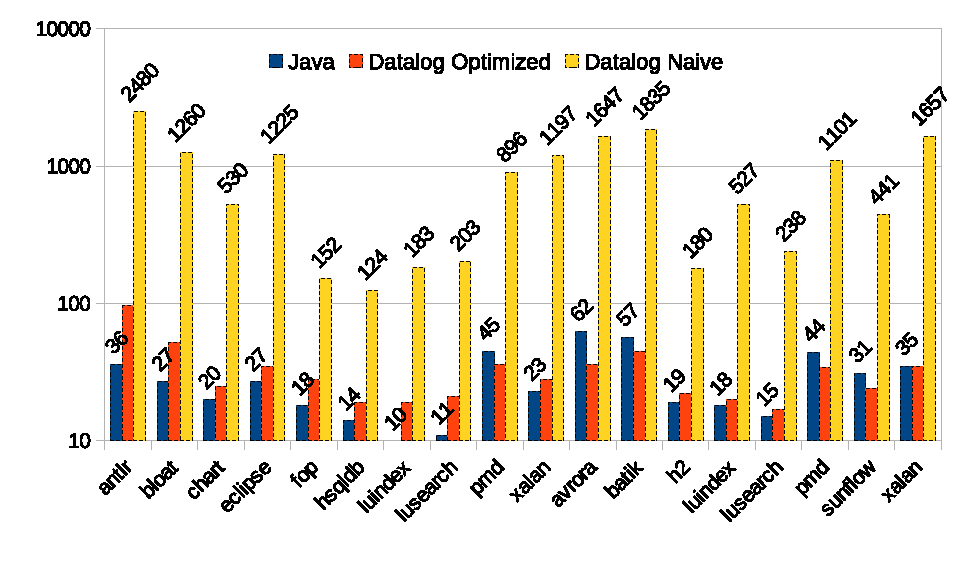
\includegraphics[clip,width=0.77\linewidth, height=0.4275\linewidth]{time.eps}
%%   \end{minipage}
%%   \caption{Execution time (sec.) of the analysis. We only show the numbers for the Java and Datalog naive versions, to avoid crowding the chart.}
%%     \label{fig:time}
%% \end{figure*}
%% 
%% \begin{figure*}[h]
%%   \begin{minipage}[b]{\linewidth}
%%     \centering
%%     % left bottom right top
%%     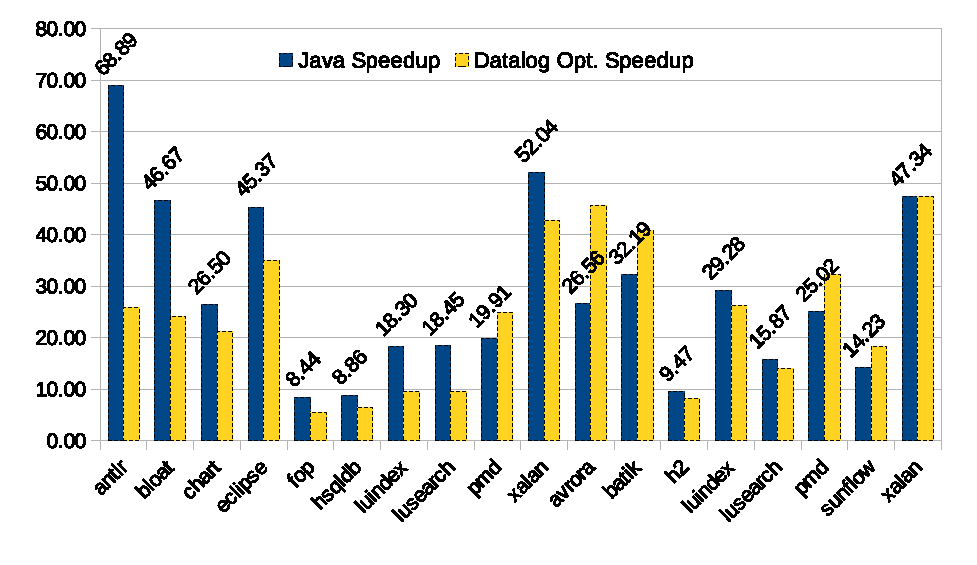
\includegraphics[clip,width=0.77\linewidth, height=0.4275\linewidth]{speedup.eps}
%%   \end{minipage}
%%   \caption{Speedup of the two analyses employing optimized data structure.}
%%     \label{fig:speedup}
%% \end{figure*}
%% 
%% 
%% 
%% It is not hard to see why the explicit representation is not competitive.
%% Figure~\ref{fig:pairs} correlates the number of aliased access-path pairs
%% (computed by the original analysis) and execution time.  (This applies to
%% context-qualified access paths, in the application and libraries alike, as long
%% as the library code is reachable from application code with the given context
%% depth.) This metric reflects the size (in tuples) of the corresponding relation
%% in the Datalog database. It clearly suggest that maintaining access path
%% relationships explicitly can prove quite costly.
%% 
%% \begin{figure}[h]
%%   \begin{minipage}[b]{\linewidth}
%%     \centering
%%     % left bottom right top
%%     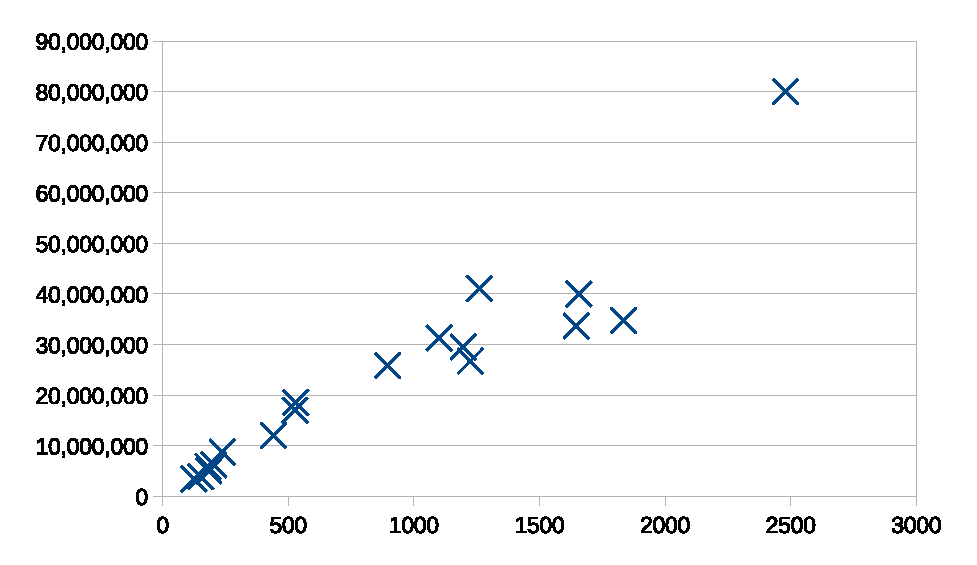
\includegraphics[clip,width=\linewidth]{pairs.eps}
%%   \end{minipage}
%%   \caption{Number of pairs of (instruction-and-context-qualified) access paths that must alias vs. analysis time.}
%%     \label{fig:pairs}
%% \end{figure}
%% 
%% %% Furthermore, the setup
%% %% explicitly downplays the benefits of our optimized data structure:
%% %% First, the ``optimized'' running time also includes import time and
%% %% computing must-point-to results for checking the equivalence of
%% %% analyses.  The latter is quite costly, since it requires re-expanding
%% %% the compactly-preserved access paths. The true computation times of
%% %% the optimized analysis are about one-third of the times listed in
%% %% Figure~\ref{fig:time}. Second, the configuration parameters (context
%% %% depth of 1 and access paths of at most length 2) are very modest, to
%% %% present the explicit representation in the best possible (while still
%% %% realistic) light. Changing these parameters can incur dramatic
%% %% slowdowns for the explicit representation, as we examine next.
%% 
%% 
%% \paragraph{Varying access-path length.} To further see the performance
%% advantage of the optimized representation of must-alias information, one can
%% vary the maximum access path length allowed for computations of the original,
%% explicit (Datalog) implementation.  Figure~\ref{fig:aplength} shows how running
%% time varies for maximum access path lengths of 2, 3 (same as in
%% Figure~\ref{fig:time}), 4 and 5. The numbers are for the xalan benchmark. The
%% speedup readily grows to over 75x for an allowed access path length of 5. The
%% optimized Datalog implementation is shown as a baseline although it should be
%% (and is) largely unaffected by the change of maximum access path length.
%% 
%% \begin{figure}[h]
%%   \begin{minipage}[b]{\linewidth}
%%     \centering
%%     % left bottom right top
%%     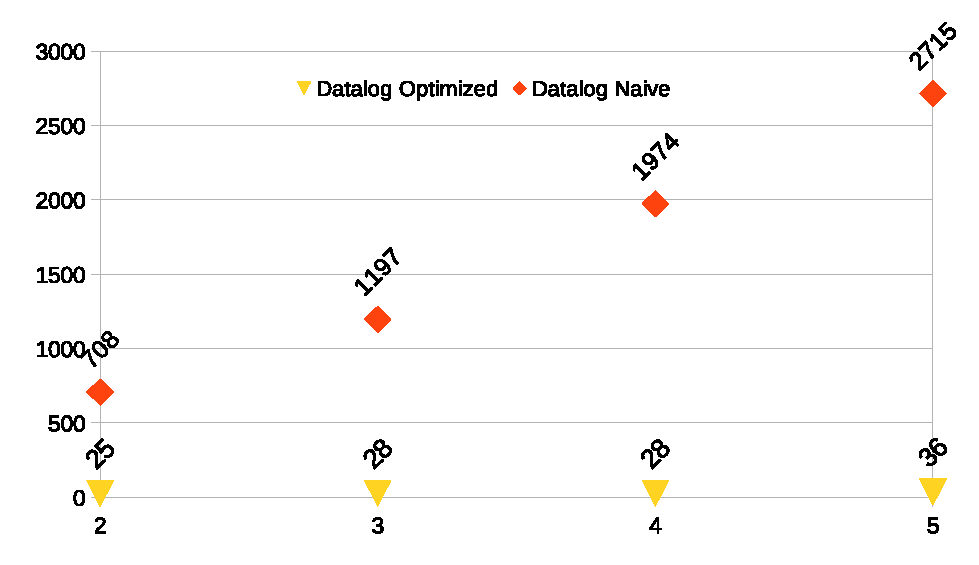
\includegraphics[clip,width=\linewidth]{length.eps}
%%   \end{minipage}
%%   \caption{Execution time when varying maximum access-path length. Optimized
%%     Datalog running time given as a baseline.}
%%     \label{fig:aplength}
%% \end{figure}
%% 
%% 
%% %for which the optimized representation achieved the \emph{lowest} speedup (14x) in Figure~\ref{fig:time}.
%% 
%% 
%% %% \begin{figure}
%% %%   \setlength{\tabcolsep}{6pt}
%% %%   \centering
%% %%   \begin{tabular}{||l| r| r| r| r| r||}
%% %%     \toprule
%% %%   Access path   &      optimized &      explicit & speedup  & must-alias & access path         \\
%% %%     length      & time  (sec)    & time (sec)    &          &  \#pairs   &  must-point-to   \\
%% %%                 &                &               &          &    (Ks)    &  \# entries  (Ks)\\
%% %%     \midrule
%% %%     1 &     47 & 290	                         & 6.2      & 	3399    & 	1953  \\
%% %%     2 &     47 & 658	                         & 14.0     & 	9979    &   1969  \\
%% %%     3 &     47 & 1521                            & 32.4     & 18528    & 	1971  \\
%% %%     \bottomrule
%% %%   \end{tabular}
%% %%   \caption{Analysis results (for the xalan benchmark) when varying the
%% %%     maximum access path length. This restriction does not affect our
%% %%     optimized implementation, whose running time is included in every
%% %%     row only for reference.}
%% 
%% %%   \label{fig:aplength}
%% %% \end{figure}
%% 
%% 
%% \paragraph{Varying context depth.} Similar observations can be made by varying
%% the context depth of the analysis. As seen in Figure~\ref{fig:ctxdepth},
%% although the running time of the optimized implementation grows slowly, the
%% running time of the explicit representation of alias relationships gets
%% dramatically higher. For a context depth of 4, the explicit representation did
%% not terminate after one-and-a-half hour.
%% 
%% \begin{figure}[h]
%%   \begin{minipage}[b]{\linewidth}
%%     \centering
%%     % left bottom right top
%%     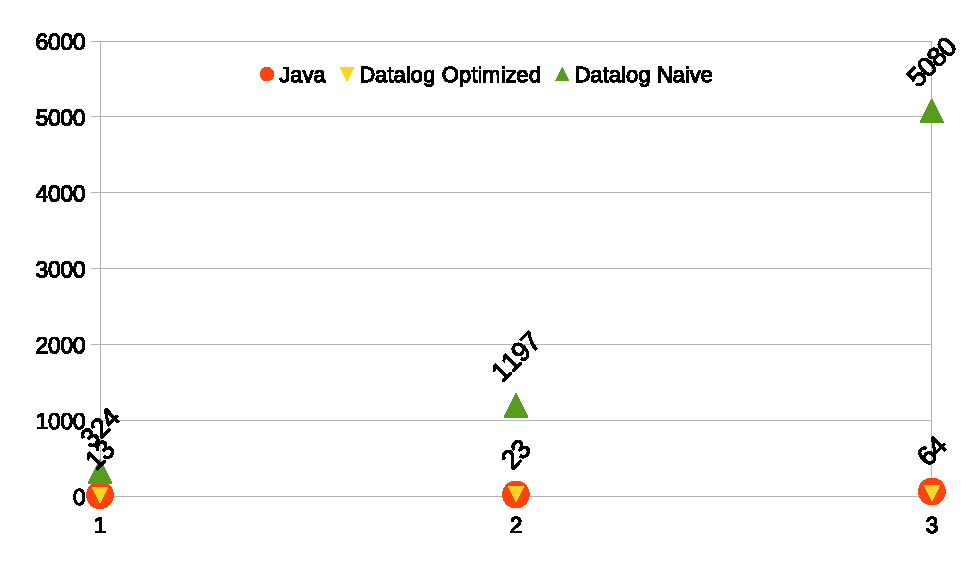
\includegraphics[clip,width=\linewidth]{depth.eps}
%%   \end{minipage}
%%   \caption{Execution time when varying maximum context depth.}
%%     \label{fig:ctxdepth}
%% \end{figure}
%% 
%% 
%% %% \begin{figure}
%% %%   \setlength{\tabcolsep}{6pt}
%% %%   \centering
%% %%   \begin{tabular}{||l| r| r| r| r| r||}
%% %%     \toprule
%% %%     Context   &      optimized &      explicit & speedup & must-alias & access path         \\
%% %%     depth     & time  (sec)    & time (sec)    &         &  \#pairs   &  must-point-to   \\
%% %%               &                &               &         &    (Ks)    &  \# entries (Ks) \\
%% %%     \midrule
%% %%     0 &  45 & 	92  & 	2.0	 &  1177 & 	1794 \\  
%% %%     1 &  47 & 	658 & 	14.0 & 	9979 & 	1969 \\  
%% %%     2 &  56 & 	1449&	25.9 &  33439&	2610 \\  
%% %%     \bottomrule
%% %%   \end{tabular}
%% %%   \caption{Analysis results (for the xalan benchmark) when varying the maximum
%% %%    context depth of the analysis.}
%% 
%% %%   \label{fig:context}
%% %% \end{figure}
%% 
%% Recall the two claimed benefits of the optimized representation: long access
%% paths are represented implicitly, and equivalence classes are represented with
%% linear space and time complexity, instead of quadratic. It is the latter factor
%% that comes into play when context depth increases: alias sets grow in size, by
%% exploiting inter-procedural inference (e.g., aliasing established at the caller
%% and propagated through formal arguments) in addition to local instructions.
%% 
%% In all, the optimized representation fulfills its promise of a much more
%% economical representation of must-alias (equivalence) relations. 
%% 
%% 
%% 
%% %% The minimal model of earlier sections captures the essence of our
%% %% full-fledged implementation. Our framework, \textsc{MaDoop}, is built
%% %% on top of the \textsc{Doop} Datalog framework for may-point-to
%% %% analysis of Java bytecode~\cite{oopsla/BravenboerS09}. Whereas
%% %% \textsc{Doop} is a flow-insensitive points-to analysis framework
%% %% (ignoring the order of instructions in a method), \textsc{MaDoop} adds
%% %% flow-sensitive modeling of the Java bytecode program (a full
%% %% control-flow graph over basic blocks). All program structure
%% %% information is represented as logical tables, which are subsequently
%% %% processed by about 300 logical rules.
%% 
%% 
%% %% To demonstrate the framework experimentally, we apply it to the DaCapo
%% %% benchmark programs~\cite{dacapo:paper} v.2006-10-MR2 under JDK
%% %% 1.7.0\_21.  We use the LogicBlox Datalog engine, v.3.10.19, on a Xeon
%% %% E5530 2.4GHz machine with only one thread running at a time and 24GB
%% %% of RAM.  When a may-analysis is needed, we employ the most precise
%% %% analysis that scales to large programs in the \textsc{Doop}
%% %% framework---a 2-object-sensitive analysis with a context-sensitive
%% %% heap (2objH).
%% 
%% %% We study five of the DaCapo benchmarks: antlr, chart, luindex,
%% %% lusearch, pmd. We wanted a small enough set for human inspection of
%% %% alias pairs at select program points, as well as programs for which a
%% %% 2objH analysis terminates. The scalability of our own must-alias
%% %% analysis is not a concern: as discussed earlier, a must-alias analysis
%% %% is naturally incremental. Hence, scalability to large programs is largely not
%% %% an issue: we can apply the analysis to just the application classes or
%% %% to a smaller hand-selected subset of the program code.
%% 
%% %% Figure~\ref{fig:info} presents statistics on the sizes of the
%% %% benchmarks, in terms of application code deemed reachable by the
%% %% \textsc{Doop} may-point-to analysis (2objH), as well as the running
%% %% time of this analysis. We also include the execution time for the
%% %% preparatory computation over the may-analysis results (``must
%% %% pre-analysis'' column)---i.e., the time to compute our
%% %% required input predicates, \altrelname{Resolved},
%% %% \altrelname{MayAlias} and \altrelname{CallMayStoreToField}.
%% 
%% %% %% \begin{figure}[t]
%% %% %%   \small
%% %% %%   \centering
%% %% %%   \begin{tabular}{lrrrrr}
%% %% %%     \toprule
%% %% %%     &&&& \multicolumn{2}{c}{may analysis time}
%% %% %%     \\
%% %% %%     \cmidrule(lr){5-6}
%% %% %%     Bench. & instructions & methods & classes & core (2objH) & must
%% %% %%                                                                   pre-analysis
%% %% %%     \\
%% %% %%     \midrule
%% %% %%     antlr    & 65518 & 1638 & 229 &  7m48s & 3m41s \\ %.18s \\
%% %% %%     chart    & 29126 & 1176 & 516 & 18m46s & 4m21s \\ %.07s \\
%% %% %%     luindex  & 19732 &  693 & 351 &   4m5s & 1m51s \\ %.90s \\
%% %% %%     lusearch & 26473 & 1049 & 351 &  4m28s & 1m58s  \\ %.78s \\
%% %% %%     pmd      & 49114 & 1880 & 554 &  5m25s & 3m18s \\ %.22s \\
%% %% %%     \bottomrule
%% %% %%   \end{tabular}
%% %% %%   \caption{Statistics for reachable application code, 2objH
%% %% %%     may-point-to analysis and must pre-analysis.}
%% %% %%   \label{fig:info}
%% %% %% \end{figure}
%% 
%% %% \begin{figure}[t]
%% %%   \small
%% %%   \centering
%% %%   \begin{tabular}{lrrrr}
%% %%     \toprule
%% %%     &&& \multicolumn{2}{c}{may analysis time}
%% %%     \\
%% %%     \cmidrule(lr){4-5}
%% %%     Benchmark & methods & classes & core (2objH) & must
%% %%                                                                   pre-analysis
%% %%     \\
%% %%     \midrule
%% %%     antlr    & 1638 & 229 &  7m48s & 3m41s \\ %.18s \\
%% %%     chart    & 1176 & 516 & 18m46s & 4m21s \\ %.07s \\
%% %%     luindex  &  693 & 351 &   4m5s & 1m51s \\ %.90s \\
%% %%     lusearch & 1049 & 351 &  4m28s & 1m58s  \\ %.78s \\
%% %%     pmd      & 1880 & 554 &  5m25s & 3m18s \\ %.22s \\
%% %%     \bottomrule
%% %%   \end{tabular}
%% %%   \caption{Statistics for reachable application code, 2objH
%% %%     may-point-to analysis and must pre-analysis.}
%% %%   \label{fig:info}
%% %% \end{figure}
%% 
%% %% Our must-alias analysis is run with a maximum access path length of
%% %% 3. Context depth varies per experiment, as discussed below.
%% 
%% %% \paragraph{Comparison with Intra-Procedural Analysis.}
%% 
%% %% As a first measure of the value of our inter-procedural must-alias
%% %% analysis, we compare it against intra-procedural analyses. Traditional
%% %% compilers can already compute aliases using intra-procedural data-flow
%% %% analysis and employ them for optimizations such as common
%% %% subexpression elimination, constant folding, or register allocation.
%% %% It is interesting to consider whether there is benefit from considering
%% %% more precisely the effects of called methods, in order to infer more
%% %% local aliases.
%% 
%% %% For this experiment, we ran our analysis algorithm (with a context
%% %% depth of 1) over the entire application portion of the
%% %% benchmarks. That is, the size of our \consname{RootMethod} set is the
%% %% number of methods shown in Figure~\ref{fig:info}.
%% 
%% %% The first and last settings shown in Figure~\ref{fig:exp1} (``intra-procedural'' and
%% %% ``inter-procedural'', respectively) present a
%% %% purely intra-procedural analysis and our full inter-procedural
%% %% algorithm.
%% %% %The former is
%% %% %produced from our framework with the inter-procedural propagation
%% %% %rules disabled. 
%% %% The intra-procedural analysis does not exploit aliasing
%% %% inferences from other methods, and conservatively invalidates alias
%% %% pairs at method calls and heap stores.
%% 
%% %% \begin{figure*}[t]
%% %%   \small
%% %%   \centering
%% %%   \begin{tabular}{lrcrrcrrcrrcr}
%% %%     \toprule
%% %%     \multicolumn{13}{c}{\normalsize \emph{Alias pairs}} \\
%% %%     % \cmidrule(l){2-13}
%% %%     \midrule
%% %%     & \multicolumn{3}{c}{intra-procedural}
%% %%     & \multicolumn{3}{c}{intra-proc.$^{+\text{may}}$}
%% %%     & \multicolumn{3}{c}{inter-proc.$_{-\text{may}}$}
%% %%     & \multicolumn{3}{c}{inter-procedural} \\
%% %%     \cmidrule(lr){2-4} \cmidrule(lr){5-7} \cmidrule(lr){8-10} \cmidrule(l){11-13}
%% %%     & \multirow{2}{2em}{per insn.} & \multirow{2}{2em}{per ret.} & time
%% %%     & \multirow{2}{2em}{per insn.} & \multirow{2}{2em}{per ret.} & time
%% %%     & \multirow{2}{2em}{per insn.} & \multirow{2}{2em}{per ret.} & time
%% %%     & \multirow{2}{2em}{per insn.} & \multirow{2}{2em}{per ret.} & time
%% %%     \\ Bench. \\
%% %%     \midrule
%% %%     antlr    &  7 &  3 & 1m37s & 41 &  6 & 3m21s &  34 & 19 & 14m25s & 105 & 27 & 37m37s \\
%% %%     chart    & 10 &  4 & 1m37s & 15 &  6 & 1m34s &  26 & 20 &  3m31s & 34 & 24  &  4m57s \\
%% %%     luindex  &  4 &  3 & 0m36s &  7 &  6 & 0m59s &   7 &  7 &  1m26s & 12 & 12  &  1m34s \\
%% %%     lusearch &  5 &  3 & 0m53s &  6 &  5 & 0m54s &   8 &  6 &  1m22s & 12 & 10  &  1m56s \\
%% %%     pmd      & 13 &  3 & 2m26s & 15 &  4 & 2m19s &  23 & 17 &  7m59s & 27 & 19  &  9m39s \\
%% %%     \bottomrule
%% %%   \end{tabular}
%% %%   \caption{Average \#alias pairs per program element (divided by 2,
%% %%     i.e., with equivalent symmetric pairs removed), and timings for
%% %%     various settings.}
%% %%   \label{fig:exp1}
%% %% \end{figure*}
%% 
%% %% The main metric to watch for in this comparison is ``alias
%% %% pairs per instruction'', i.e., the first of the three columns in every
%% %% grouping of numbers. As can be seen, the full inter-procedural analysis
%% %% (last of the four settings shown in Figure~\ref{fig:exp1}) yields
%% %% significantly richer information than the intra-procedural analysis
%% %% (first setting). With only intra-procedural information, we can infer
%% %% at most one half, and often less than one third, of the alias pairs.
%% %% The alias pairs shown are unconditional (i.e., for context
%% %% \consname{All}) with symmetric pairs removed. The numbers are over the
%% %% Jimple intermediate language of the Soot framework and, thus, the
%% %% alias pairs are more numerous than one would expect from program
%% %% inspection, due to the introduction of several temporary
%% %% variables. 
%% 
%% %% \begin{figure*}[t]
%% %%   \small
%% %%   \centering
%% %%   \begin{tabular}{lrrrrrr}
%% %%     \toprule
%% %%     & \multicolumn{3}{c}{\emph{Alias pairs} under 1-must-context}
%% %%     & \multicolumn{3}{c}{\emph{Alias pairs} under 5-must-context} \\
%% %%     \cmidrule(lr){2-4} \cmidrule(lr){5-7}
%% %%     Benchmark & per instr. & per all-return & time
%% %%               & per instr. & per all-return & time
%% %%     \\
%% %%     \midrule
%% %%     antlr    & 10 &  8 & 0m51s & 19 & 12 &  2m48s \\
%% %%     chart    & 25 & 13 & 1m25s & 30 & 18 &  1m21s \\
%% %%     luindex  &  8 &  6 & 0m20s &  9 &  7 &  0m25s \\
%% %%     lusearch &  6 &  5 & 0m22s &  9 &  7 &  1m12s \\
%% %%     pmd      &  6 &  4 & 0m25s & 11 &  9 & 10m12s \\
%% %%     \bottomrule
%% %%   \end{tabular}
%% %%   \caption{Alias pairs (with equivalent symmetric pairs removed, i.e., numbers divided by 2), and timings
%% %%   for different contexts of the must-alias analysis.}
%% %%   \label{fig:exp2}
%% %% \end{figure*}
%% 
%% 
%% %% \paragraph{Value of May-Analysis for Must- Inference.}
%% 
%% %% Figure~\ref{fig:exp1} shows two more settings of our analysis:
%% %% intra-procedural$^{+\text{may}}$ and inter-procedural$_{-\text{may}}$.
%% %% These help us quantify how exactly may-analysis information
%% %% contributes to the must-analysis.
%% 
%% %% The intra-procedural$^{+\text{may}}$ setting does intra-procedural
%% %% must-alias reasoning but invalidates access paths by employing the
%% %% inter-procedural may-alias analysis. That is, of the three predicates
%% %% computed by the may-analysis, the intra-procedural$^{+\text{may}}$
%% %% analysis does \emph{not} use predicate \altrelname{Resolved} to do
%% %% virtual method resolution, but \emph{does} use predicates
%% %% \altrelname{MayAlias} and \altrelname{CallMayStoreToField}, in order
%% %% to decide when to invalidate access paths at call and store
%% %% instructions. 
%% %% %
%% %% Conversely, the inter-procedural$_{-\text{may}}$ analysis \emph{does}
%% %% use predicate \altrelname{Resolved} to do virtual method resolution,
%% %% but does \emph{not} use predicates \altrelname{MayAlias} and
%% %% \altrelname{CallMayStoreToField}, instead invalidating alias
%% %% information conservatively at store and call instructions.
%% 
%% %% These variations of settings give us a picture of the separate benefit
%% %% from various kinds of inter-procedurality (may vs. must reasoning).
%% %% As can be seen, inter-procedural reasoning benefits greatly from both
%% %% kinds of inter-procedural may-analysis information. 
%% %% %%SPACE
%% %% %The inter-procedural$_{-\text{may}}$ setting is significantly less
%% %% %effective than the full inter-procedural analysis, while still
%% %% %typically much better than intra-procedural$^{+\text{may}}$, which, in
%% %% %turn, is better than the purely intra-procedural setting.
%% %% %
%% %% %%SPACE
%% %% Note that all of the above configurations were produced via
%% %% straightforward configuration of our full implementation.
%% %% This is testament to the inherent configurability of a modular,
%% %% declarative framework.
%% %% %This ease of
%% %% %experimentation is testament to the inherent configurability of a
%% %% %modular, declarative framework, as opposed to a monolithic
%% %% %implementation.
%% 
%% %% \paragraph{Timings.}
%% 
%% %% Figure~\ref{fig:exp1} also shows the running time for our analysis, as
%% %% well as for intra-procedural analyses. As can be seen, the must-alias
%% %% analysis is quite fast. In the case of antlr, the analysis time blows up,
%% %% but so do the inferred facts. Generally, our timings do not aim
%% %% to reflect an ideal implementation of the declarative
%% %% rules. Specifically, our Datalog
%% %% engine does not use union-find trees for the equivalence classes of
%% %% reflexively and transitively closed relations, thus incurring
%% %% significant overhead.
%% %% %We have tried to minimize such overhead within the parameters allowed
%% %% %by the execution engine but a manual implementation can likely fare
%% %% %better. 
%% %% On the other hand, our implementation is heavily optimized in terms of
%% %% rule execution and indexing (for fast combination of relations), to an
%% %% extent that a manual implementation will have difficulties matching.
%% 
%% 
%% %% \paragraph{Results for Human Inspection.}
%% 
%% %% For human inspection of aliases, we have found it useful to produce
%% %% all alias pairs that hold (unconditionally, i.e., under an
%% %% \consname{All} context) for \emph{all} return statements of a method.
%% %% This ``forall'' intersection of aliasing information over all
%% %% return sites offers a good summary of the method's effects, and
%% %% is more concise than alias information at a single given
%% %% instruction.
%% 
%% %% Figure~\ref{fig:exp1} shows the sizes of the sets computed in this
%% %% fashion, as the second of the three columns for every analysis
%% %% setting.  As can be seen, the full inter-procedural must-alias
%% %% analysis is again significantly more information-rich than any other
%% %% setting. The sizes of the resulting alias sets (from 10 to 27)
%% %% are small enough for human inspection and typically
%% %% quite informative.
%% 
%% 
%% 
%% %% \paragraph{Exploring Parts of the Program, Using Context.}
%% 
%% %% To explore parts of the program only conditionally (with alias pairs
%% %% qualified by context), we selected at random 20 methods in each of the
%% %% benchmarks. We ran the analysis with these methods in the
%% %% \consname{RootMethod} set, and different maximum context depth values,
%% %% to allow exploration of code outside that set as much as the context
%% %% depth permits.
%% 
%% %% Figure~\ref{fig:exp2} shows the result of this experiment, for context
%% %% depth settings of 1 and 5. The alias pairs shown are computed \emph{at
%% %%   the root methods only}, i.e., they do not count alias pairs in the
%% %% methods analyzed under a non-\consname{All} context, but they do count
%% %% the impact of such methods on the alias information at the original
%% %% root method set.
%% 
%% %% The execution time demonstrates the incrementality of the must-alias
%% %% analysis---its running time was often negligible.
%% %% %%SPACE
%% %% % (Recall that much of
%% %% %the time shown is spent computing queries over the \emph{may-}
%% %% %analysis, in order to populate input tables \altrelname{Resolved},
%% %% %\altrelname{MayAlias}, and \altrelname{CallMayStoreToField}, and not
%% %% %on the must-alias analysis itself.)
%% 
%% %% For a deeper context, the analysis produces often significantly richer
%% %% facts. Since the methods of origin are randomly selected, the number of
%% %% extra alias pairs (when mapped back at the root
%% %% methods) varies, but is generally consistent.


\section{Related Work}
\label{sec:related}

There are several approaches in the literature that present
must-analyses in the pointer analysis setting or employ them in a
may-analysis. Our approach is a must-alias analysis applied to Java
bytecode, but conceptually it is distinguished by its minimizing the
distance between the implementation and the declarative specification.
%% and by its leveraging of a highly-efficient data structure for sets of
%% alias classes.

%% Ma et al.~\cite{DBLP:conf/isola/MaWD08} present an algorithm for
%% null-pointer dereference detection using a
%% context-insensitive may-alias and a must-alias analysis; the latter is
%% used to increase the precision of the former, by enabling strong
%% updates when possible.

Nikoli\'{c} and Spoto~\cite{DBLP:conf/ictac/NikolicS12} present a
must-alias analysis that tracks aliases between program expressions
and local variables (or stack locations, since they analyze Java
bytecode%% , which is a stack-based representation
).  The analysis
%itself does not expose any clear configuration points but it 
is related to ours both because of its application to Java bytecode
and because it is constraint-based: the analysis is a generator of
constraints, which are subsequently solved to produce the analysis
results.
% Abstractly,
%this is a relative of our Datalog-based approach, but it is unclear
%how the two may compare in terms of engineering tradeoffs.

Hind et al. \cite{Hind:1999:IPA:325478.325519} present a collection of pointer
analysis algorithms. Among them, the most relevant to this work is a
flow-sensitive interprocedural pointer alias analysis. The authors
optimistically produce \emph{must} information for pointers to single
non-summary objects.

Emami et al.~\cite{emami-etal-pldi94} present an approach that
simultaneously calculates both must- and may-point-to information for
a C analysis. Their empirical results ``show the existence of a
substantial number of definite points-to relationships, which forms
very valuable information''---much in line with our own
experience.

Must- information is often computed in conjunction with a
client analysis. One of the best examples is the typestate
verification of Fink et al.~\cite{1146254}, which demonstrates the value of
a must-analysis and the techniques that enable it.

The analysis of \cite{De:2012:SFP:2367163.2367203} is essentially a
flow-sensitive may-point-to analysis that performs strong updates, as
it maps \emph{access paths} to \emph{heap objects} (abstracted by
their allocation sites). 
The approach uses a flow-insensitive
may-point-to analysis to bootstrap the main analysis. However, it
provides no \emph{definite} knowledge of any sort, since the aim is to
increase the precision of the may-analysis. For instance, even if an
access path points to a single heap object, according to the De and
D'Souza analysis, there is no \emph{must} point-to information
derived, since this object could be a summary object (i.e., one that
abstracts many objects allocated at the same allocation site). To
reason about such cases, other approaches, such as the more expensive
shape analysis algorithms \cite{mattmight:Sagiv:2002:TVLA},
additionally maintain summary information per heap object. In this
way, they allow must point-to edges to exist only if the target is
definitely not a summary node.

%An alternative approach to handle this shortcoming is to propagate
%% An approach for integrating \emph{must} point-to reasoning in an
%% analysis is to propagate such
%% %\emph{must}-point-to 
%% information only at instructions where we know that the given heap
%% allocation target still refers to the last object allocated at that
%% site \cite{Altucher:1995:EFM:199448.199466}. Thus, an execution path
%% that may create another object at the same site (such as when reaching
%% the end of the loop) would invalidate any previous must-point-to facts
%% (i.e., it will stop them from propagating any further).

Generally, must-analyses can vary greatly in sophistication and can be
employed in an array of different combinations with may-analyses.  The
analysis of Balakrishnan and Reps~\cite{sas/BalakrishnanR06}, which
introduces the \emph{recency abstraction}, distinguishes between the
most recently allocated object at an allocation site (a concrete
object, allowing strong updates) and earlier-allocated objects
(represented as a summary node). The analysis additionally keeps
information on the size of the set of objects represented by a summary
node. At the extreme, one can find full-blown shape analysis
approaches, such as that of Sagiv et
al.~\cite{mattmight:Sagiv:2002:TVLA}, which explicitly maintains must-
and may- information simultaneously, by means of three-valued truth
values, in full detail up to predicate abstraction: a
relationship can definitely hold (``must''), definitely not hold
(``must not'', i.e., negation of ``may''), or possibly hold
(``may''). Summary and concrete nodes are again used to represent
knowledge, albeit in full detail, as captured by arbitrary predicates
whose value is maintained across program statements, at the cost of a
super-exponential worst-case complexity.

%% Jagannathan et al.~\cite{Jagannathan:1998:SLM:268946.268973} present
%% an algorithm for must-alias analysis of functional languages. The
%% algorithm adapts must-alias insights to the setting of captured
%% variables.
%% %captured in closures.  
%% For instance, must-alias information for
%% non-summary objects permits strong updates, which the authors find to
%% improve analysis precision. We employ must-alias analysis results
%% quite similarly in applications of our model analysis.


%% Our optimized data structure is (partly) based on the observation that
%% must-alias sets are equivalence classes. This is not the first time
%% that a data structure that efficiently implements equivalence classes
%% has been used to speed up pointer analysis. Most notably, a
%% Steensgaard-style (or \emph{unification-based})
%% \cite{steensgard:1996:PointsTo} analysis computes may-point-to sets
%% that are equivalence classes. This means that points-to sets are
%% disjoint---if two points-to sets are found to possibly overlap, they
%% get unified. This loses precision (relative to a standard subset-based
%% points-to analysis) but enables the algorithm to use union-find trees
%% for a very efficient representation.

%% Another optimized data structure often used in pointer analysis is the
%% \emph{constraint graph}: a graph with nodes denoting pointer variables
%% and an edge between nodes \code{p} and \code{q} denoting flow (e.g., a
%% direct assignment) from variable \code{p} to variable \code{q}.  Online
%% cycle elimination by F\"{a}ndrich et al.
%% \cite{pldi/FahndrichFSA98} detects cycles in the
%% constraint graph and collapses all nodes in a cycle into a
%% representative node, since such nodes will have identical points-to
%% information. The technique of Nasre
%% \cite{ismm/Nasre12} extends such constraint graph
%% reasoning based on the observation that if two nodes have the same
%% dominator in the constraint graph, then they are clones: the values
%% flowing to them are (only) those of the dominator node. Several other
%% constraint graph optimizations are applied off-line (i.e., before the
%% points-to analysis runs).  Prime examples of such techniques are
%% Rountev and Chandra's \cite{rountevOffline} and Hardekopf and Lin's
%% \cite{hardekopfOffline}. (Hardekopf and Lin have also applied similar
%% ideas in a hybrid online/offline setting \cite{antgrasshopper}.)  Both
%% of these techniques perform an off-line detection of equivalent
%% points-to sets and use this knowledge to eliminate redundant work in
%% subsequent points-to computations. Our data structure can be seen as
%% somewhat analogous to constraint-graph techniques, in the sense that
%% we do not compute the flow of objects or the fully expanded set of all
%% possible alias pairs. Instead, we compute the ``wiring'' (i.e., the
%% alias relationships, locally, that the program induces) and keep the
%% alias information in condensed form, until it needs to be queried by a
%% client analysis.

%% %Hardekopf and
%% %Lin's approach is impressively general, computing hash codes that
%% %encode all the logical processing of a points-to set that is induced
%% %by the current program and, thus, detecting equivalent points-to sets
%% %even through complex program patterns.

%% % \citep{Heintze:2001:UAA:378795.378855} ; pre-transitive constraint-graph and reachability caching



%% \section{Conclusions}
%% \label{sec:conclusions}

%% We presented a declarative algorithm model for an inter-procedural
%% must-alias analysis over access paths, and a data structure for its
%% optimized implementation. The algorithmic improvements afforded
%% by the specialized data structure yield a tremendous performance
%% advantage, often approaching two orders of magnitude.

%% The literature on must-alias analyses is sparse and the distance of
%% specification to implementation is typically large. In our literature
%% survey we have not found a single must-alias analysis publication that
%% concretely refers to another and shows how its approach differs. Thus,
%% we believe that our declarative model can offer a reference point for
%% future work. Accompanied by our proposed data structure, the model can
%% spur further discussion on how to make must-alias analyses more
%% complete and how to implement them efficiently.

%\newpage

%% We believe that our model is clear yet concrete
%% enough to spur further development and a better understanding of the
%% comparative features of different must-alias analysis algorithms. In
%% practical terms, must-alias analysis is valuable and woefully
%% under-exploited in the literature. Our experiments show concrete value
%% for (human) program understanding and (automatic) optimization.


%% discussed its features and configurability options.  The
%% model faithfully reflects \textsc{MaDoop}: a full-fledged
%% implementation of more than 300 Datalog rules to analyze Java
%% bytecode. Our analysis interfaces with the may-point-to analyses of
%% the \textsc{Doop} framework and can leverage their precision, at
%% clearly defined interaction points.

\chapter{Must-Alias Analysis: Data Structures}\label{chapter:must-data}
\chapter{Defensive Points-To Analysis}\label{chapter:defensive}
%Defensive Points-To Analysis: Effective Soundness via Laziness

\part{Epilogue}
\chapter{paNda: a Datalog compiler}\label{chapter:panda}
\chapter{Related Work}
\label{chapter:related}
\epigraph{Hermits United. We meet up every 10 years, swap stories about caves. It’s good fun… for a hermit.}{\textit{The 10th Doctor} - Doctor Who}

%This chapter includes related work of previous chapters (Chapter~\ref{chapter:hybrid}-\ref{chapter:defensive}).

\section{Hybrid Context-Sensitivity}

We have discussed directly related work throughout Chapter~\ref{chapter:hybrid}. Here we selectively mention a few techniques that, although not directly related to ours, offer alternative approaches to sweet spots in the precision/performance tradeoff.

Special-purpose combinations of context-sensitivity have been used in the past, but have required manual identification of classes to be treated separately (e.g., Java collection classes, or library factory methods). An excellent representative is the TAJ work for taint analysis of Java web applications \cite{pldi:2009:Tripp}. In contrast, we have sought to map the space and identify interesting hybrids for general application of context-sensitivity, over the entire program.

The analyses we examined are context-sensitive but flow-insensitive. We can achieve several of the benefits of flow-sensitivity by applying the analysis on the static single assignment (SSA) intermediate form of the program. This is easy to do with a mere flag setting on the \doop{} framework. However, the impact of the SSA transformation on the input is minimal. The default intermediate language used as input in \doop{} (the Jimple representation of the Soot framework \cite{cascon:1999:Vall,cc:2000:Vall}) is already close to SSA form, although it does not guarantee that every variable is strictly single-assignment without requesting it explicitly. Published work by Lhot\'{a}k and Chung \cite{popl:2011:Lhotak} has shown that much of the benefit of flow-sensitivity derives from the ability to do strong updates of the points-to information. Lhot\'{a}k and Chung then exploited this insight to derive analyses with similar benefit to a full flow-sensitive analysis at lower cost.

A demand-driven evaluation strategy reduces the cost of an analysis by computing only those results that are necessary for a client program analysis~\cite{oopsla:2005:Sridharan,pldi:2006:Sridharan,popl:2008:Zheng,pldi:2001:Heintze}. This is a useful approach for client analyses that focus on specific locations in a program, but if the client needs results from the entire program, then demand-driven analysis is typically slower than an exhaustive analysis.

Reps~\cite{cc:1994:Reps} showed how to use the standard magic-sets optimization to automatically derive a demand-driven analysis from an exhaustive analysis (like ours). This optimization combines the benefits of top-down and bottom-up evaluation of logic programs by adding side-conditions to rules that limit the computation to just the required data.

An interesting recent approach to demand-driven analyses was introduced by Liang and Naik \cite{pldi:2011:Liang}. Their ``pruning'' approach consists of first computing a coarse over-approximation of the points-to information, while keeping the provenance of this derivation, i.e., recording which input facts have affected each part of the output. The input program is then pruned so that parts that did not affect the interesting points of the output are eliminated. Then a precise analysis is run, in order to establish the desired property.



\section{Introspective Analysis}
\label{sec:related:introspective}

The effort to tune the context-sensitivity of an analysis is pervasive in the literature. Nevertheless, most approaches fundamentally differ from ours of Chapter~\ref{chapter:introspective}, either by trying to vary context-sensitivity based on syntactic properties or by trying to focus on only a part of the program that matters for answering a given query. In contrast, we attack the context-sensitive scalability problem  head-on, in the all-points points-to analysis setting, with context used all over the program and library.

Typical scalable points-to analysis frameworks such as textsc{Wala}~\cite{www:wala} and \doop{}~\cite{oopsla:2009:Bravenboer} employ a multitude of low-level heuristics for tuning the precision and scalability of an analysis. These include using extra context for collection classes, using a heap context for arrays in an analysis without a context-sensitive heap, allocating strings or exceptions context-insensitively, treating library factory methods with deeper context, etc. Such heuristics are typically user-selected and prominent in the documentation of the respective frameworks, and have also appeared in the literature (e.g., \cite{pldi:2009:Tripp,cc:2013:Kastrinis}). However, all such approaches are mere hard-wired heuristics and do not address the major scalability problem that our approach aims to solve. The scalability issues identified in earlier literature and discussed throughout this paper are present after all such heuristics have been employed.

A more general approach is the hybrid context-sensitivity of Chapter~\ref{chapter:hybrid}. Such a hybrid analysis attempts to emulate call-site sensitivity for static method calls and object-sensitivity for dynamic calls. The approach becomes interesting when context is deep (e.g., how are context elements merged when a dynamic call is made inside a static call?). Nevertheless, the hybrid context-sensitivity approach does not change the essence of the problem we are trying to solve. For hard-to-analyze applications, hybrid context-sensitive algorithms are equally unscalable as their component algorithms. For the purposes of our experimental study, which only tests the scalability of heavyweight benchmarks, hybrid context-sensitivity is virtually indistinguishable from object-sensitivity.

In recent years there have been many more instantiations of introspective analysis, with very different metrics of cost and benefit. These modern instantiations outperform our original Heuristic-A and Heuristic-B but keep the same flavor: \textsc{Zipper}~\cite{oopsla:2018:Li} aims to achieve mostly-guaranteed precision with heuristically better scalability, whereas \textsc{Scaler}~\cite{esec-fse:2018:Li} achieves guaranteed scalability and typically significantly better precision than a context-insensitive analysis.

More interesting applications of selective context-sensitivity have been explored in the context of \emph{demand-driven} pointer analysis. A demand-driven evaluation strategy reduces the cost of an analysis by computing only those results that are necessary for a client program analysis~\cite{oopsla:2005:Sridharan,pldi:2006:Sridharan,popl:2008:Zheng,pldi:2001:Heintze}. This is a useful approach for client analyses that focus on specific locations in a program, but if the client needs results from the entire program, then demand-driven analysis is typically slower than an exhaustive analysis.

In the demand-driven space, refinement-based analyses have been used primarily in the work of Sridharan and Bod\'{\i}k~\cite{pldi:2006:Sridharan} and of Liang and Naik~\cite{pldi:2011:Liang}. Sridharan and Bod\'{\i}k introduce refinement-based analysis as a way to adaptively increase the precision characteristics of an existing analysis algorithm when a client analysis is not satisfied with the result. The approach allows turning on field-sensitivity, as well as higher call-site sensitivity for an analysis algorithm. Yet, unlike ours, it is not a general approach that can apply to any kind of context and a large number of different algorithms. Liang and Naik's ``pruning'' approach consists of first computing a coarse over-approximation of the points-to information, while keeping the provenance of this derivation, i.e., recording which input facts have affected each part of the output. The input program is then pruned so that parts that did not affect the interesting points of the output are eliminated. Then a highly context-sensitive precise analysis is run, in order to establish the desired property. This approach is similar to introspective context-sensitivity in that the analysis is run twice and a separate query over the first-run result determines the second run's characteristics. Nevertheless, our approach requires no provenance computation (which is unlikely to scale for an all-points analysis) and works even when we want answers for the entire program---i.e., when pruning is not possible.

Both of the above demand-driven approaches can be viewed as complements of our introspective context-sensitivity. In the demand-driven world, it is possible to estimate the \emph{benefit} that a more precise analysis may yield: either the client is happy with the current level of precision (which implies there is no further benefit to be obtained) or it is not, in which case more precision should be added. In our all-points pointer analysis problem we have no such information. This motivates our \emph{cost}-based heuristics, which attempt to estimate ``what can go wrong'' when more precision gets added, as opposed to ``what can be gained'', as in demand-driven techniques.



\section{Must-Alias Analysis}

\subsection*{Logical Model}

There are several approaches in the literature that present must-analyses in the pointer analysis setting or employ them in a may-analysis. Our approach is a must-alias analysis applied to Java bytecode, but conceptually it is distinguished by its minimizing the distance between the implementation and the declarative specification.

Ma et al.~\cite{isola:2008:Ma} present an algorithm for null-pointer dereference detection using a context-insensitive may-alias and a must-alias analysis; the latter is used to increase the precision of the former, by enabling strong updates when possible.

Nikoli\'{c} and Spoto~\cite{ictac:2012:Nikolic} present a must-alias analysis that tracks aliases between program expressions and local variables (or stack locations, since they analyze Java bytecode, which is a stack-based representation). The analysis is related to ours both because of its application to Java bytecode and because it is constraint-based: the analysis is a generator of constraints, which are subsequently solved to produce the analysis results. Abstractly, this is a relative of our Datalog-based approach, but it is unclear how the two may compare in terms of engineering tradeoffs.

Hind et al. \cite{article:1999:Hind} present a collection of pointer analysis algorithms. Among them, the most relevant to this work is a flow-sensitive interprocedural pointer alias analysis. The authors optimistically produce \emph{must} information for pointers to single non-summary objects.

Emami et al.~\cite{pldi:1994:Emami} present an approach that simultaneously calculates both must- and may-point-to information for a C analysis. Their empirical results ``show the existence of a substantial number of definite points-to relationships, which forms very valuable information''---much in line with our own experience.

The analysis of \cite{ecoop:2012:De} is essentially a flow-sensitive may-point-to analysis that performs strong updates, as it maps \emph{access paths} to \emph{heap objects} (abstracted by their allocation sites). The approach uses a flow-insensitive may-point-to analysis to bootstrap the main analysis. However, it provides no \emph{definite} knowledge of any sort, since the aim is to increase the precision of the may-analysis. For instance, even if an access path points to a single heap object, according to the De and D'Souza analysis, there is no \emph{must} point-to information derived, since this object could be a summary object (i.e., one that abstracts many objects allocated at the same allocation site). To reason about such cases, other approaches, such as the more expensive shape analysis algorithms \cite{article:2002:Sagiv}, additionally maintain summary information per heap object. In this way, they allow must point-to edges to exist only if the target is definitely not a summary node.

Must- information is often computed in conjunction with a client analysis. One of the best examples is the typestate verification of Fink et al.~\cite{issta:2006:Fink}, which demonstrates the value of a must-analysis and the techniques that enable it.

An approach for integrating \emph{must} point-to reasoning in an analysis is to propagate such information only at instructions where we know that the given heap allocation target still refers to the last object allocated at that site \cite{popl:1995:Altucher}. Thus, an execution path that may create another object at the same site (such as when reaching the end of the loop) would invalidate any previous must-point-to facts (i.e., it will stop them from propagating any further).

Generally, must-analyses can vary greatly in sophistication and can be employed in an array of different combinations with may-analyses. The analysis of Balakrishnan and Reps~\cite{sas:2006:Balakrishnan}, which introduces the \emph{recency abstraction}, distinguishes between the most recently allocated object at an allocation site (a concrete object, allowing strong updates) and earlier-allocated objects (represented as a summary node). The analysis additionally keeps information on the size of the set of objects represented by a summary node. At the extreme, one can find full-blown shape analysis approaches, such as that of Sagiv et al.~\cite{article:2002:Sagiv}, which explicitly maintains must- and may- information simultaneously, by means of three-valued truth values, in full detail up to predicate abstraction: a relationship can definitely hold (``must''), definitely not hold (``must not'', i.e., negation of ``may''), or possibly hold (``may''). Summary and concrete nodes are again used to represent knowledge, albeit in full detail, as captured by arbitrary predicates whose value is maintained across program statements, at the cost of a super-exponential worst-case complexity.

Jagannathan et al.~\cite{popl:1998:Jagannathan} present an algorithm for must-alias analysis of functional languages. The algorithm adapts must-alias insights to the setting of captured variables in closures. For instance, must-alias information for non-summary objects permits strong updates, which the authors find to improve analysis precision. We employ must-alias analysis results quite similarly in applications of our model analysis.


\subsection*{Data Structures}

Our optimized data structure is (partly) based on the observation that must-alias sets are equivalence classes. This is not the first time that a data structure that efficiently implements equivalence classes has been used to speed up pointer analysis. Most notably, a Steensgaard-style (or \emph{unification-based}) \cite{popl:1996:Steensgaard} analysis computes may-point-to sets that are equivalence classes. This means that points-to sets are disjoint---if two points-to sets are found to possibly overlap, they get unified. This loses precision (relative to a standard subset-based points-to analysis) but enables the algorithm to use union-find trees for a very efficient representation.

Another optimized data structure often used in pointer analysis is the \emph{constraint graph}: a graph with nodes denoting pointer variables and an edge between nodes \code{p} and \code{q} denoting flow (e.g., a direct assignment) from variable \code{p} to variable \code{q}. Online cycle elimination by F\"{a}ndrich et al. \cite{pldi:1998:Fahndrich} detects cycles in the constraint graph and collapses all nodes in a cycle into a representative node, since such nodes will have identical points-to information. The technique of Nasre \cite{ismm:2012:Nasre} extends such constraint graph reasoning based on the observation that if two nodes have the same dominator in the constraint graph, then they are clones: the values flowing to them are (only) those of the dominator node. Several other constraint graph optimizations are applied off-line (i.e., before the points-to analysis runs). Prime examples of such techniques are Rountev and Chandra's \cite{pldi:2000:Rountev} and Hardekopf and Lin's \cite{sas:2007:Hardekopf}. (Hardekopf and Lin have also applied similar ideas in a hybrid online/offline setting \cite{pldi:2007:Hardekopf}.) Both of these techniques perform an off-line detection of equivalent points-to sets and use this knowledge to eliminate redundant work in subsequent points-to computations. Our data structure can be seen as somewhat analogous to constraint-graph techniques, in the sense that we do not compute the flow of objects or the fully expanded set of all possible alias pairs. Instead, we compute the ``wiring'' (i.e., the alias relationships, locally, that the program induces) and keep the alias information in condensed form, until it needs to be queried by a client analysis.

Another conceptual relative of our data structure is the model presented by Madhavan et al. \cite{article:2015:Madhavan} for modular \emph{may} analyses. That model is similar in that it invents abstract nodes for heap objects that resemble ours (without the equivalence-class nature). The Madhavan et al. approach aims to achieve modular reasoning, i.e., to model the heap effects of a method without knowing its calling environment. To do so, the approach creates abstract nodes that represent concepts such as ``whichever object variable \code{x} may point to''. Our data structure has nodes with a similar meaning, however we also take advantage of the ``must'' nature of the analysis to merge nodes, every time the same access path can reach both.



\section{Defensive Analysis}
\label{sec:related:defensive}

There is certainly past work that attempt to ensure a sound whole-program analysis, but none matches the generality and applicability of our approach. We selectively discuss representative approaches.

The standard past approach to soundness for a careful static analysis has been to ``bail out'': the analysis detects whether there are program features that it does not handle soundly, and issues warnings, or refuses to produce answers. This is a common pattern in abstract-interpretation~\cite{popl:1977:Cousot} analyses, such as Astr\'{e}e~\cite{sas:2007:Delmas}, which have traditionally emphasized sound handling of conventional language features. However, this is far from a solution to the problem of being sound for opaque code: refusing to handle the vast majority of realistic programs can be argued to be sound, but is not usefully so. In contrast, our work handles \emph{all} realistic programs, but returns partial (but sound) results, i.e., produces non-empty points-to sets for a subset of the variables. It is an experimental question to determine whether this subset is usefully large, as we do in our evaluation.

Hirzel et al. \cite{ecoop:2004:Hirzel,article:2007:Hirzel} use an online pointer analysis to deal with reflection and dynamic loading by monitoring their run-time occurrence, recording their results, and running the analysis again, incrementally. However, this is hardly a \emph{static} analysis and its cost is prohibitive for precise (context-sensitive) analyses, if applied to all reflection actions.

Lattner et al. \cite{pldi:2007:Lattner} offer an algorithm that can apply to incomplete programs, but it assumes that the linker can know all callers (i.e., there is no reflection---the analysis is for C/C++) and the approach is closely tied to a specific flow-insensitive, unification-based analysis logic~\cite{popl:1996:Steensgaard}, necessary for simultaneously computing inter-related points-to, may-alias, and may-escape information.

Sreedhar et al. \cite{pldi:2000:Sreedhar} present the only past approach to explicitly target dynamic class loading, although only for a specific client analysis (call specialization). Still, that work ends up making many statically unsound assumptions (requiring, at the very least, programmer intervention), illustrating well the difficulty of the problem, if not addressed defensively. The approach assumes that only the public API of a ``closed world'' is callable, thus ignoring many uses of reflection. (With reflection, any method is callable from unknown code, and any field is accessible.) It ``[does] not address the Java features of reloading and the Java Native Interface''. It ``optimistically assumes'' that ``[the extant state of statically known objects] remains unchanged when they become reachable from static reference variables''. It is not clear whether the technique is conservative relative to adversarial native code (in system libraries, since the JNI is ignored). Finally, the approach assumes the existence of a sound may-point-to analysis, even though none exists in practice!

Traditional conservative call-graph construction (\emph{Class Hierarchy Analysis (CHA)} \cite{ecoop:1995:Dean} or \emph{Rapid Type Analysis (RTA)} \cite{oopsla:1996:Bacon}) is unsound. Such algorithms explore the entire class hierarchy for matching (overriding) methods and consider all of them to be potential virtual call targets. However, even this is not sufficient for a sound static analysis of opaque code: classes can be generated and loaded dynamically during program execution. CHA cannot find target methods that do not even exist statically, yet modeling them is precisely what is needed for soundness in real-world conditions. For instance, Java applications, especially in the enterprise (server-side) space, employ dynamic loading heavily, and patterns such as \emph{dynamic proxies} have been standardized and used widely since the early Java days.

Furthermore, such heuristic ``best-effort'' over-approximation is detrimental to analysis precision and performance. CHA is an example of a loose over-approximation in an effort to capture most dynamic behaviors.
(Similar loose over-approximations have been proposed, for instance, for reflection analysis~\cite{aplas:2015:Smaragdakis}.) Loose over-approximations compute many more possible targets than those that realistically arise. This yields vast points-to sets that render the analysis heavyweight and useless due to imprecision. (Avoiding such costs is exactly why past analyses have often opted for glaringly unsound handling of opaque code features.) Our lazy representation of ``don't know''/''cannot bound'' values as empty sets addresses the problem, by keeping all points-to sets compact.

The conventional handling of reflection in may-point-to analysis algorithms for Java~\cite{www:wala-reflection,ecoop:2014:Li,aplas:2005:Livshits,thesis:Livshits,aplas:2015:Smaragdakis,sas:2015:Li} is unsound, instead relying on a ``best-effort'' approach.  Such past analyses attempt to statically model the result of reflection operations, e.g., by computing a superset of the strings that can be used as arguments to a \code{Class.forName} operation (which accepts a name string and returns a reflection object representing the class with that name). The analyses are unsound when faced with a completely unknown string: instead of assuming that \emph{any} class object can be returned, the analysis assumes that \emph{none} can. The reason is that over-approximation (assuming any object is returned) would be detrimental to the analysis performance and precision. Even with an unsound approach, current algorithms are heavily burdened by the use of reflection analysis. For instance, the documentation of the \textsc{Wala} library directly blames reflection analysis for scalability shortcomings \cite{www:wala-reflection},\footnote{The \textsc{Wala} documentation is explicit: ``\emph{Reflection usage and the size of modern libraries/frameworks make it very difficult to scale flow-insensitive points-to analysis to modern Java programs. For example, with default settings, textsc{Wala}'s pointer analyses cannot handle any program linked against the Java 6 standard libraries, due to extensive reflection in the libraries.}''~\cite{www:wala-reflection}} and enabling reflection on the \doop{} framework slows it down by an order of magnitude on standard benchmarks~\cite{aplas:2015:Smaragdakis}. Furthermore, none of these approaches attempt to model dynamic loading---a ubiquitous feature in Java enterprise applications.
\chapter{Conclusions and Future Work}\label{chapter:conclusions}

\backmatter

\end{document}